% These commented lines make the thesis look good as a standalone document
% \documentclass[a4paper,11pt]{report}
% \usepackage[tmargin=2.5cm,bmargin=2.5cm,lmargin=2.8cm,rmargin=2.8cm,headheight=0cm]{geometry}

% these two lines are to make the thesis printable in a book (with alternate spacing)
\documentclass[epsfig,a4paper,11pt,titlepage,twoside,openany]{book}
\usepackage[paperheight=29.7cm,paperwidth=21cm,outer=1.5cm,inner=2.5cm,top=2cm,bottom=2cm]{geometry}

\usepackage{epsfig}
\usepackage{plain}
\usepackage{setspace}
\usepackage{titlesec}

\usepackage[T2A,T1]{fontenc}
\usepackage[utf8]{inputenc}
\usepackage[russian, english]{babel}

\usepackage{todonotes}
\usepackage{cite} \graphicspath{ {graphics/} }
\usepackage{csquotes}

\usepackage{amsmath}
\usepackage{algorithm,algorithmic}
\usepackage{array}

\usepackage[colorlinks=true,linkcolor=black,citecolor=blue]{hyperref}
 
\usepackage{tabularx}
\usepackage{multirow}
\usepackage{float}
\usepackage{makecell}
\usepackage[capitalise]{cleveref}
\usepackage{amssymb}

\usepackage{longtable}
\usepackage{lscape}
\usepackage{subcaption}

\usepackage[inline]{enumitem}

\usepackage{listings}
\usepackage{xcolor}
 
\definecolor{codegreen}{rgb}{0,0.6,0}
\definecolor{codegray}{rgb}{0.5,0.5,0.5}
\definecolor{codepurple}{rgb}{0.58,0,0.82}
\definecolor{backcolour}{rgb}{0.95,0.95,0.95}
\definecolor{dkgreen}{rgb}{0,0.6,0}
\definecolor{mauve}{rgb}{0.58,0,0.82}
\definecolor{mgray}{rgb}{0.5,0.5,0.5}

\lstdefinestyle{mystyle}{
    backgroundcolor=\color{backcolour},   
    aboveskip=5mm,
    belowskip=5mm,
    showstringspaces=false,
    columns=flexible,
    basicstyle={\ttfamily},
    numberstyle=\tiny\color{mgray},
    numbers=left,
    numbersep=5pt,
    keywordstyle=\color{blue},
    commentstyle=\color{dkgreen},
    stringstyle=\color{mauve},
    breaklines=true,
    breakatwhitespace=true,
    tabsize=2, 
    sensitive = true,
    escapeinside={(*}{*)},
    frame=single,
    language=Python,
}

\lstset{style=mystyle}

\newcommand{\footurl}[1]{\footnote{\url{#1}}}
\newcommand{\soweego}[0]{\texttt{soweego}}

\linespread{1.25}

\begin{document}
\pagenumbering{gobble} \pagestyle{plain}

\thispagestyle{empty}

\begin{center}
	
	\begin{figure}[!h]
		\centering
		
\includegraphics[width=0.6\textwidth]{logo_unitn}
	\end{figure}
	
  \vspace{2 cm} 

  \LARGE{Department of Information Engineering and Computer Science\\}

  \vspace{1 cm} 
  \Large{Master’s Degree in\\
    Computer Science
  }

  \vspace{3 cm} 
  \Large\textsc{FINAL DISSERTATION\\} 
  \vspace{1 cm} 

  \Huge\textsc{soweego:\\}
  \Large{\it{ensemble learning applied to record linkage}}


  \vspace{2 cm} 
  \begin{tabular*}{\textwidth}{ l @{\extracolsep{\fill}} r }
    \Large{Supervisor:} & \Large{Student:}\\
    \Large{Andrea Passerini}& \Large{Andrea Tupini}\\
    \Large{Marco Fossati }
  \end{tabular*}

  \vspace{3 cm} 
  
  \Large{Accademic Year 2018/2019}
  
\end{center}



\clearpage

\listoftodos
\todo[inline]{make all hyperlinks black}

%%%%%%%%%%%%%%%%%%%%%%%%%%%%%%%%%%%%%%%%%%%%%%%%%%%%%%%%%%%%%%%%%%%%%%%%%%
%%%%%%%%%%%%%%%%%%%%%%%%%%%%%%%%%%%%%%%%%%%%%%%%%%%%%%%%%%%%%%%%%%%%%%%%%%
%% Nota
%%%%%%%%%%%%%%%%%%%%%%%%%%%%%%%%%%%%%%%%%%%%%%%%%%%%%%%%%%%%%%%%%%%%%%%%%%
%% Sezione Ringraziamenti opzionale
%%%%%%%%%%%%%%%%%%%%%%%%%%%%%%%%%%%%%%%%%%%%%%%%%%%%%%%%%%%%%%%%%%%%%%%%%%
%%%%%%%%%%%%%%%%%%%%%%%%%%%%%%%%%%%%%%%%%%%%%%%%%%%%%%%%%%%%%%%%%%%%%%%%%%
\thispagestyle{empty}

\begin{center}
  {\bf \Huge Acknowledgements}
\end{center}

\vspace{4cm}



\textit{First of all I want to thank my family for their support and constant motivation. Especially my parents, without who's help I wouldn't be able be here. To my in-laws, for their help, suggestions, and support.}

\textit{I also want to thank my supervisors, Andrea Passerini, and Marco Fossati, for the invaluable guidance they provided during this whole process. }

\textit{To my wife, Kate, for her constant encouragement and understanding. For putting up with me and basically keeping me alive this past few months.}

%\textit{I want to thank the Wikipedia community for  a grant to this work, and for their supportive comments.}

\textit{Finally, I want to thank all the open source community who made this work possible .}


\clearpage
\pagestyle{plain}
  
\mainmatter

%%%%%%%%%%%%%%%%%%%%%%%%%%%%%%%%%%%%%%%%%%%%%%%%%%%%%%%%%%%%%%%%%%%%%%%%%%
%%%%%%%%%%%%%%%%%%%%%%%%%%%%%%%%%%%%%%%%%%%%%%%%%%%%%%%%%%%%%%%%%%%%%%%%%%
%% Nota
%%%%%%%%%%%%%%%%%%%%%%%%%%%%%%%%%%%%%%%%%%%%%%%%%%%%%%%%%%%%%%%%%%%%%%%%%%
%% Si ricorda che il numero massimo di facciate e' 30. Nel conteggio delle
%% facciate sono incluse indice sommario capitoli Dal conteggio delle facciate
%% sono escluse frontespizio ringraziamenti allegati
%%%%%%%%%%%%%%%%%%%%%%%%%%%%%%%%%%%%%%%%%%%%%%%%%%%%%%%%%%%%%%%%%%%%%%%%%%
%%%%%%%%%%%%%%%%%%%%%%%%%%%%%%%%%%%%%%%%%%%%%%%%%%%%%%%%%%%%%%%%%%%%%%%%%%

% indice
\tableofcontents
\clearpage
    
    
          
% gruppo per definizone di successione capitoli senza interruzione di pagina
\begingroup



% Template styles nessuna interruzione di pagina tra capitoli ridefinizione dei
% comandi di clear page
\renewcommand{\cleardoublepage}{} \renewcommand{\clearpage}{}
% redefinizione del formato del titolo del capitolo da formato Capitolo X Titolo
% capitolo a formato X Titolo capitolo
      
\titleformat{\chapter} {\normalfont\Huge\bfseries}{\thechapter}{1em}{}
        
\titlespacing*{\chapter}{0pt}{0.59in}{0.02in}
\titlespacing*{\section}{0pt}{0.20in}{0.02in}
\titlespacing*{\subsection}{0pt}{0.10in}{0.02in}
% end template style


% ---------- Below are MY styles
% % % nessuna interruzione di pagina tra capitoli ridefinizione dei comandi di
% % % clear
% % % page
% \renewcommand{\cleardoublepage}{}
% % \renewcommand{\clearpage}{}
% % % redefinizione del formato del titolo del capitolo da formato Capitolo X
% % % Titolo
% % % capitolo a formato X Titolo capitolo
      
% \titleformat{\chapter} {\normalfont\Huge\bfseries}{\thechapter}{1em}{}
% \titlespacing*{\chapter}{0pt}{0pt}{0.17in}
% \titlespacing*{\section}{0pt}{0.20in}{0.09in}
% \titlespacing*{\subsection}{0pt}{0.10in}{0.08in}

% \setlength\abovedisplayshortskip{5pt} \setlength\belowdisplayshortskip{15pt}
% \setlength\abovedisplayskip{5pt} \setlength\belowdisplayskip{15pt}
% ------------ End my styles

%%%%%%%%%%%%%%%%%%%%%%%%%%%%%%%% 

\chapter{Introduction}
\label{chap:introduction}

% from template
% Sommario è un breve riassunto del lavoro svolto dove si descrive l'obiettivo,
% l'oggetto della tesi, le metodologie e le tecniche usate, i dati elaborati e la
% spiegazione delle conclusioni alle quali siete arrivati.

% Il sommario dell’elaborato consiste al massimo di 3 pagine e deve contenere le
% seguenti informazioni:

% \begin{itemize}
% \item contesto e motivazioni
% \item breve riassunto del problema affrontato
% \item tecniche utilizzate e/o sviluppate
% \item risultati raggiunti, sottolineando il contributo personale del laureando/a
  
% \end{itemize}
% end from template

% ---------------------------
% draft
% ---------------------------

\todo[inline,color=green!25]{Work in progress}

This project's goal is to aid in the development of the
\texttt{soweego}\footurl{https://meta.wikimedia.org/wiki/Grants:Project/Hjfocs/soweego}
, which is a data importing system that adds references to Wikipedia
pages.

\texttt{soweego} was developed as an answer to the amount of Wikipedia pages that
do not have reliable external references, which are necessary to ensure data
quality. Specifically, its aim is to align the Wikidata entities with a set of
external databases (catalogs).


\section{A brief overview of Wikidata}
\label{sec:intro-wikidata}

\textit{Wikidata} is defined as the \textit{knowledge base} that supports
\textit{Wikipedia} and all of the \textit{Wikimedia Foundation}
projects\footurl{https://wikimediafoundation.org/}. A \textit{knowledge base} is a collection of statements of and about the world. There are many different knowledge bases available on the web but, \textit{Wikidata} is one of the most complete out there, it also has a very active and extense community of users and volunteers. 

In this specific \textit{knowledge base} there are different \textit{items} which are interconnected and integrated with each other. They achieve this through the use of a \textit{Wikidata} construct called 
\textit{properties}. 

Each \textit{item} is identified by using a special tag named \texttt{QID} (Q-identifier), it was given this name because each of these unique values starts with the letter \textit{Q}. Information about a specific item (QID) is
recorded by the use of \textit{statements} which are \textit{key-value} pairs
that contain specific information about each item.

The key of each statement is a \textit{property}, and the value can be a reference to another item via its QID, a string, a number, or media
files\footurl{https://www.wikidata.org/wiki/Help:Statements}. Statements can
also be extended by the use of \textit{qualifiers} which are \textit{extra information} about the
statement. An example of this can be a person who studied at some university for
a certain period of time (this period of time would be the qualifier).

Properties\footurl{https://www.wikidata.org/wiki/Help:Properties}, like items,
have their own ID. These are known as \texttt{PID} (Property-ID). Some properties may accept only one value, or multiple values, and
some may also be constrained in some specific way: for example, its value can
only be a string composed of one letter.

In Wikidata both \textit{items} and \textit{properties} are associated with a name and a
brief description, the main difference is how they are used: items, have the
goal of representing a specific entity while properties, are used to express 
information regarding said entity. Another difference between them would be that \textit{items} are displayed on their respective page on Wikipedia and \textit{properties} are not.

Consider the QID \textit{Q42}, which identifies the writer
\textit{Douglas Adams}. Below is a table representing which shows some of the statements about him
using QIDs and PIDs.

\begin{table}[H]
  \centering
  \begin{tabular}{l|l}
    PID                                & QID                   \\ \hline
    P31 (instance of)                  & Q5 (human)            \\ \hline
    P21 (sex)                          & Q6581097 (male)       \\ \hline
    P19 (place of birth)               & Q350 (Cambridge)      \\ \hline
    \multirow{3}{*}{P106 (occupation)} & Q28389 (screenwriter) \\ \cline{2-2} 
                                       & Q6625963 (novelist)   \\ \cline{2-2} 
                                       & Q245068 (comedian)   
  \end{tabular}
  \caption{Wikidata statements describing Douglas Adams}
  \label{tab:intro-wikidata-douglas42}
\end{table}

Here it is possible to see that this way of expressing information is very
flexible and allows for a quick and rich construction of knowledge. 





%%%%%%%%%%%%%%%%%%%%%%%%%%%%%%%% 

\chapter{State of the art}
\label{chap:state-of-the-art}

This chapter will mainly cover \textit{Record Linkage}, a standard method used to link a pair of databases. The next section will give a brief introduction to the record linkage workflow, and mention some of the most common terms used in this document. \autoref{sec:rl-as-a-workflow} will show how record linkage can be thought of as a pipeline, and every step will be explained in depth. Finally, \autoref{sec:rl-related-work} will mention related work.

\section{Introduction to Record Linkage}
\label{sec:rl-intro}

\textit{Record linkage} is commonly used when there is a need for data integration. This is achieved by finding pairs of records which represent the same underlying \textit{entity}, and by joining them according to a previously defined set of criteria. It is possible to apply the technique both for, connecting a pair of databases (which we call \textit{catalogs} in this use case) and for removing duplicates from one single catalog.

  

For a more formal description of the problem, suppose there are two datasets ($\Psi$ and $\Omega$). The goal of record linkage is to find all those pairs $(x, y)$ where $x \in \Psi$ and $y \in \Omega$, such that both $x$ and $y$ refer to the same underlying entity. Hence, the algorithm must compare the entities from $\Psi$ and $\Omega$, and decide which of them are a match (i.e., refer to the same underlying entity) and which are not. 
Record Linkage can also be naturally expressed or viewed as a problem of clustering, in which the objective is to cluster all the entities representing the same \textit{latent entity} together.

The goal, as defined in \cite{fellegi69_theor_recor_linkag}, is to find two different sets $M$ and $U$, where $M$ is composed of all matching pairs and $U$ contains all non-matching ones:

\begin{align*}
  M &= \{(x, y); x = y; x \in \Psi; y \in \Omega\} \\
  U &= \{(x, y); x \neq y; x \in \Psi; y \in \Omega\}
\end{align*}

The problem of joining different catalogs is trivial when the catalogs have a
shared, unique identifier. For example, when joining the datasets of
customers from two banks, and each customer is associated with their government
ID, or some other unique identifier. In this case, it is just a matter of
matching on this attribute and merging the resulting pairs.

However, it is commonly the case (as is the case for this project as well), that
catalogs do not have a common unique identifying attribute, thus requiring a less trivial approach.

As shown later in this chapter (\autoref{sec:rl-main-approaches}), there are two main methods of performing record linkage, but basically they can be separated into methods which match directly comparing pairs of fields, and methods which measure the similarity between said pairs.

Besides not having a unique identifier, it may also be the case that the datasets that need to be merged, have some mistakes. This is something which is especially noticeable when we are working with data representing people. These are some of the mistakes that might come up: 

\begin{itemize}
\item The names were misspelled.
\item The first and last names are reversed.
\item The format of the date is not standardised.
\item The dates presented are simply not possible, since they are too forward in the future or too far in the past.
\end{itemize}

Many of these can be somewhat reduced by preprocessing the dataset, but others may not, and it is necessary to account for them when working with the data.

To give an example of a situation in which \textit{record linkage} would be used,
suppose there are two databases of clients which need to be joined for some company. The tables below represent said databases.

\begin{table}[H]
  \centering{}
  \begin{tabular}{l|l|l}
    First Name & Last Name  & Birth Year \\ \hline
    Brenda     & Williams   & 1990       \\
    Meng        & Yu         & 1950       \\
    Gary        & Crowley   &  1956 \\
    Bruno      & Lima       & 1956      
  \end{tabular}
  \caption{Example catalog from bank \#1}
  \label{tab:ex-catalog-1}
\end{table}


\begin{table}[H]
  \centering{}
  \begin{tabular}{l|l|l}
    First Name & Last Name  & Birth Year \\ \hline
    Emma       & Farr       & 1971       \\
    Yu         & Meng       & 1950       \\
    Juri       &  Petrov    & 1932 \\
    Gary       & Crowley    & 1956      
  \end{tabular}
  \caption{Example catalog from bank \#2}
  \label{tab:ex-catalog-2}
\end{table}

The catalogs above do not have a unique identifier which unequivocally links them, so it is necessary to check the attributes which are available. The fields can be compared in turn and if they all match then it can be said that two entities are the same. For example, it can be easily seen that \textit{Gary Crowley} is in both datasets since an entity with said name exists in both and their birth dates match. On the other hand, nothing can be confidently said about the other possible matches since for none of them all the fields match. There is a pair (\textit{Meng Yu} in the first dataset, and \textit{Yu Meng} in the second) which might be the same person since the names are similar and they share a birth date. For this last instance there is no way to be sure if the first and last names are reversed in one of the dataset of if they are actually different people. This kind of situation is quite common in real-world datasets.





\subsection{Main Approaches}
\label{sec:rl-main-approaches}

There are two main approaches\footnote{Besides these two approaches, in the record linkage literature we commonly find the term \textit{clerical}, which entails \textit{manual} work, i.e., by a clerk.} to consider when talking about record linkage: 1)\textit{deterministic}, and 2) \textit{probabilistic}. 

The main difference between these is the way in which the pairs of entities are compared. A more thorough description of each method follows.


\subsubsection{Deterministic}
\label{sec:rl-approach-deterministic}

In deterministic record linkage all fields are compared to see if they match. If the fields do match, then it can be said that these entities are the same. However, if any of the fields that are being compared only partially match, then the pair is considered as a non-match. 

Take for instance the task of joining a catalog which provides information regarding where someone
lives with another catalog that provides their age. Both catalogs only contain the
name of the person as an identifying feature, so a composition of
these two fields (attributes) can be used to identify each entity.

\begin{table}[H]
  \centering{}
  \begin{tabular}{|l|l|l|l|}
    First Name & Last Name & Age \\ \hline
    Sarah & Miller & 42 \\
    John  & Piers  & 35  \\ 
  \end{tabular}
  \caption{Deterministic example, catalog 1}
  \label{tab:ex-deterministic-1}
\end{table}


\begin{table}[H]
  \centering{}
  \begin{tabular}{|l|l|l|l|}
    First Name & Last Name & Address \\ \hline
    Sarah  & Miller & New York \\
    Johnny & Piers  & Berlin  \\ 
  \end{tabular}
  \caption{Deterministic example, catalog 2}
  \label{tab:ex-deterministic-2}
\end{table}

After matching these results, there is a clear match for \textit{Sarah Miller}, but no available match for \textit{John Piers} and \textit{Johnny Piers}, since the
names are different and there is no way to be sure if \textit{Johnny} is just a nickname (making them the same person)
or if these two entities are actually different people.

Note also that in this example both rows coincide completely on the \textit{Last Name} field. However, when doing deterministic record linkage partial matches are not considered \cite{dusetzina_m_2014}, because there can be no uncertainty in the match.

It should be noted that this linking procedure is not optimal when the provided data is not very clean. Preprocessing steps can be taken to ensure that the catalogs are as
uniform as possible, but even so, it is never easy to know if there might be match missing or not.


\subsubsection{Probabilistic}
\label{sec:rl-approach-probabilistic}

In simple terms, probabilistic record linkage \cite{Sayers2015} compares a shared subset of fields of a given entity pair, then decides, whether the pair is a match or not, with a certainty value. The main difference with respect to \textit{deterministic record linkage} is that now it is allowed for fields to partially match.

By default, the task is achieved by comparing all entities in the source catalog with all entities in the target catalog (unless we opt for \textit{blocking}, as explained in \autoref{sec:rl-workflow-blocking}). 

In its most basic form, two entities are taken and compared in all their fields; which may then match completely if they are exactly the same, or partially match if they are similar but not exactly equal. This \textit{partial match} of the fields is measured by a percentage stating how similar they actually are. 

Any similarity metric can be used to measure partial similarity. For example, \textit{edit distance} for strings, which is basically the number of changes needed to transform one of the strings into the other in order to make them equal (either by adding, removing or updating characters). 

As a standard, if a comparison yields a 0 then it means the two fields are completely different, and if it yields a 0 they are the same, any value in between specifies how similar or how diverse the fields are.

Following the example catalogs defined in the previous section, now it is possible to compare the \textit{First Name} and \textit{Last Name} fields separately.
Suppose they are compared with a function $fc$ that provides the percentage of
letters both fields have in common.


$$
fc(s1, s2) = \frac{\| s1 \cap s2 \|}{\| s1 \cup s2 \|}
$$


It might be that both last names are exactly the same, as is with the first name for \textit{Sarah}. However, with the first name for \textit{John} it would show a similarity of only $0.8$ with \textit{Johnny}. Taking both the similarity given for the first and last names then it is possible to make a better informed final decision on whether both records should be marked as a definite match or not.  For instance, it may be said that if the average similarity assigned to all fields is greater than $0.5$ then it may be stated that a pair is a match. Under this assumptions \textit{John Piers} and \textit{Johnny Piers} will be classified as the same person.

The probabilistic record linkage approach is the one which will be implemented in this project.


\section{Record Linkage as a Workflow}
\label{sec:rl-as-a-workflow}

An abstraction which is commonly used when performing record linkage is that of viewing the problem as a workflow \cite{christen12_data}, where each step is in charge of performing a different transformation to the data. In probabilistic record linkage \cite{fellegi69_theor_recor_linkag} the resulting matches are usually segmented into three sets depending on how sure the probabilistic model was that a pair was a match or not. For example, pairs for which the certainty of the model falls in the interval $[0, 0.4]$ are \textit{non-matches}. Pairs whose certainty of a match is in $[0.4, 0.6]$ are \textit{potential matches}. And those whose certainty is in the range $[0.6, 1.0]$ are \textit{matches}.

\autoref{fig:rl-workflow} shows a graphical representation of said steps.

\begin{figure}[H]
  \centering 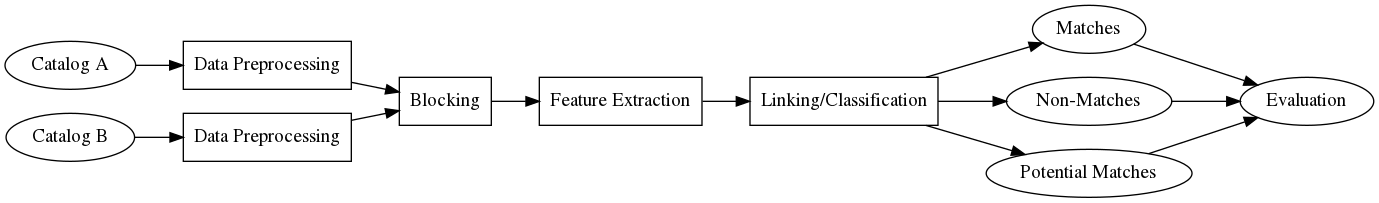
\includegraphics[width=\textwidth]{rl-workflow}
  \caption{Record linkage workflow.}
  \label{fig:rl-workflow}
\end{figure}

This process is separated into five steps and it may be applied to $n$ input catalogs, the most important part is for them to be submitted to the \textit{Data Preprocessing} step so they're as uniform and clean as possible. 



In the following sections a more in-depth description of each step will be provided.


\subsection{Data Preprocessing}
\label{sec:rl-workflow-data-preprocessing}

This is the first and most significant step in which the data is preprocessed. During this step, the catalog will be taken in and its data will be rearranged and \textit{cleaned up}. The actual meaning of this depends on the kind of data that the specific catalog
contains and it is mostly up to the designer of the system to decide in which way the presented data
should be preprocessed \cite{Rahm00datacleaning}. 
However, some of the most common cleaning procedures which are almost always done are:

\begin{enumerate}
\item Normalize the case of the text (e.g., make sure all text is lowercase).
\item Remove invalid characters for the current encoding.
\item Standardize all characters (e.g. transform accented characters into their
  \textit{non-accented} equivalent).
\item Ensure all dates comply with a given format, such as \textit{DD/MM/YYYY}.
\item Remove empty values or fill them with a default value.
\item Standardize the \textit{gender} representation. (ie, either \textit{m} or
  \textit{male})
\item Normalize names and addresses. \cite{Churches2002}
\end{enumerate}

The goal of this step is for the catalogs and their data to become as similar as possible amongst
themselves, so that there will be no need to deal with the potential differences between them once the matching process has begun.
  
It has also been shown \cite{@clark2004_rl_for_injury} that a well made data
preprocessing step is necessary for the record linkage algorithm to have positive
performance results.

For example, consider that the following data is available in some input catalogs. Note that
in this step no distinction has been made on whether the catalog is a source
catalog or not, so in this specific example the
\texttt{Catalog ID}/\texttt{Target ID} fields will be omitted.

\begin{table}[H]
  \centering

  \begin{tabular}{l|l|l}
    First Name                        & Last Name                         & Birth Date   \\ \hline
    \foreignlanguage{russian}{Анника} & \foreignlanguage{russian}{Цлаире} & 12 Sep. 1948 \\
    Abélia                            & Benoît                            & 14/4/1987    \\
    Dave                              & Smith                             & 7/28/1976   
  \end{tabular}
  
  \caption{Data preprocessing example: dirty catalog.}
  \label{tab:data-prepr-ex-dirty}
\end{table}


Before proceeding it is necessary to clean this data. Specifically, since the first entity has its first and last names written with Cyrillic letters, and the date format is different from what is expected. The second entity's first and last name use accented letters. And finally, the date of the third entity also does not respect the stated date requirements.

After passing the input catalog through the data preprocessing step the following output will be available:

\begin{table}[H]
  \centering

  \begin{tabular}{l|l|l}
    First Name & Last Name & Birth Date \\ \hline
    Annika     & Claire    & 12/9/1948  \\
    Abelia     & Benoit    & 14/4/1987  \\
    Dave       & Smith     & 28/7/1976   
  \end{tabular}
  
  \caption{Data preprocessing example: cleaned catalog.}
  \label{tab:data-prepr-ex-cleaned}
\end{table}

Notice that now all the entities conform with the required format. Once all the
catalogs have been cleaned they may be sent over to the next step of the workflow
(\textit{blocking}).



\subsection{Blocking}
\label{sec:rl-workflow-blocking}

Once the cleaned entities from the previous step are available, its necessary to define which
of them should be compared with one another. By default the pairwise comparison will be performed over all entities from all catalogs . However this can quickly
become infeasible when catalogs start getting bigger, or when their number starts to increase. 

Also, if the dataset being utilized has many different
entities then when comparing all entities against each other it will show that most of these are non matches.

% Suppose for example that we have two datasets with $100 000$ entities each. If
% we were to

It is generally the case when comparing all entities with each other then,
the number of comparison needed increases quadratically with the size of the
catalogs, while the number of true matches increases linearly
\cite{christen12_data}.

Blocking (also known as \textit{indexing}) is defined as comparing a specific entity only against entities which might be a match. When matching said entity against a dataset, its possible to use a simple rule to define a subset of all entities
composed only of those which the rule suggests are possible matches. 

This new set of entities made to be matched against is not guaranteed to contain any match, nor it
is guaranteed that none of the sets in an entity which is an actual match were left out, but it entails a much smaller number of comparisons. 
If a good blocking rule is chosen then the record linkage process becomes much more efficient.

Suppose there are two catalogs, $\Psi$ and $\Omega$, and one specific entity is being considered $x \in
\Psi$ and there is need to know which entities in the catalog $\Omega$ match with it.
Rather than comparing $x$ with the whole $\Omega$ dataset (which would result in
$\Psi \times \Omega$ comparisons), what must be done is derive a subset of possible matches using a
blocking rule $r$, which takes a pair of entities and shows if they might be a \textit{match} according to the rule or not.

$$
blocked = {y; r(x,y) = 1; y \in \Omega;}
$$

There are many possible blocking rules that can be used
\cite{christen12_survey_index_techn_scalab_recor_linkag_dedup}, ranging from the
very simple \textit{exact string match}, to the more complex phonetical q-gram
comparison of text. Usually, the more a blocking algorithm is complex the more computational power it requires. A more complex algorithm may be more precise than a simpler one. For example, a metric which compares multiple subsets of a text may be resistant to minor spelling errors, while one that compares the string character by character may not. However, the latter is less computationally expensive to perform.

These rules are applied to a pair of fields from two different entities. For
example, its possible to apply an \textit{exact string match} rule to the \textit{name}
field of two entities and see that they match if their names are exactly the
same. This simple operation makes it easy and fast to segment the dataset into
clusters of possible matches.

The decision regarding the \textit{rule} used for blocking is part of the record
linkage problem, and it needs to be simple enough so that there is an actual gain in performance, but good enough so that the resulting set of potential
matches actually includes real matches. 

Its also practical to freely use multiple blocking
rules to get multiple sets of possible matches and then use the union of these
to do the final comparisons.

The concept of \textit{blocking} has been used in record linkage almost since
the start of the field \cite{fellegi69_theor_recor_linkag}, and it is now an
integral part in most record linkage solutions \cite{winkler2006overview}. The
field of blocking is a big area of research in and of itself, with many
different methods proposed over the years
\cite{christen12_survey_index_techn_scalab_recor_linkag_dedup, Baxter2003ACO}.

However the evaluation of these methods is outside the scope of the current
work, and it will be limited to work with one of the most basic blocking rules,
known as a blocking technique which divides two strings into its corresponding
tokens, and if any of these match then it is considered for the pair to be a potential match.

For now only blocking for fields which are strings has been covered and discussed. But
blocking can be applied to many other fields as well (although strings are the
most common ones). For example, other possible ways in which blocking could be applied are: 

1) Gather all entities with a specific \textit{zip code}. 

2) Gather all entities which were born on a specific \textit{year}; etc.

Blocking is quite flexible, and is up to the designer how strict he or she wishes to make it.
Although it is agreed
\cite{christen12_survey_index_techn_scalab_recor_linkag_dedup} that it is better
to have a more \textit{lax} blocking technique which includes entities that are
not a match and later filter this out during the actual \textit{linking} step
(see \autoref{sec:rl-workflow-linking}), than using a more precise blocking but
which leaves out potential matches. 

In other words, when choosing a blocking rule its preferable to choose one which tends to include more entities than necessary, than having one which only includes few non-matches. Obviously, the choice of this trade-off needs to be done on an individual per problem basis.

As an example suppose the following two catalogs are available. They both contain the
first and last names, and the zip code of each person. The first also contains
whether said person is \textit{male} or \textit{female}, while the second catalog
contains the \textit{academic title} of each person.

\begin{table}[H]
  \centering
  \begin{tabular}{l|l|l|l|l}
    Source ID & First Name & Last Name & Zip Code & Sex \\ \hline
    A1        & Anna       & Claire    & 27321    & f   \\
    A2        & Claudio    & Bari      & 34918    & m  
  \end{tabular}
  \caption{Source Catalog: Blocking example.}
  \label{tab:blocking-ex-source}
\end{table}

\begin{table}[H]
  \centering
  \begin{tabular}{l|l|l|l|l}
    Target ID & First Name & Last Name & Zip Code & Education \\ \hline
    B1        & Annika     & Claire    & 27321    & Ph.D.     \\
    B2        & Claude     & Bari      & 34918    & Bachelor  \\
    B3        & Jane       & Stel      & 34918    & Bachelor 
  \end{tabular}
  \caption{Target Catalog: Blocking example.}
  \label{tab:blocking-ex-target}
\end{table}

Suppose the goal is to perform blocking on the \textit{Zip Code} field, and to achieve that, 
\textit{exact match} strategy is used. Its possible to see that in total there are only two zip
codes (\textit{27321} and \textit{34918}), so after blocking there will end up being two sets. The first one (for zip code \textit{27321}) will contain the pair
$[(A1, B1)]$, both of which could arguably be the same person. In the second set the remaining pairs $[(A2, B2), (A2, B3)]$ can be found.

For the first set its only necessary to compare the source entity \textit{Anna Claire}
with \textit{one} target entity. In the second the
source entity \textit{Claudio Bari} must be compared with two target entities. In both cases the
total number of comparisons for a source entity is less than what would be needed
without blocking (3 comparisons).

The gain in the example doesn't seem like much, but it is easy to imagine that
this procedure would be very effective at reducing the total number of
comparisons once the amount of zip codes and, by extension the amount of sets
generated by blocking, start to increase in number.

In short, the goal of blocking is to reduce as much as possible the number of
comparisons that each entity will be subject to by using a \textit{blocking
  rule} which finds the best potential matches for said entity in an efficient
way.

  
\subsection{Feature Extraction}
\label{sec:rl-workflow-feat-extraction}

The feature extraction step is in charge of taking a pair of entities and
extracting from them a set of \textit{features}, which characterize how similar
this pair of entities is. The pair of entities for which the features are extracted
are those pairs which the previous \textit{blocking} step said may be good
candidates for a match.

As mentioned before, each entity is composed of a series of fields. By comparing said fields, and extracting a value from each comparison, a new vector can be generated. This vector, called \textit{feature vector}, characterizes the similarity between each field of the pair of entities.

The comparison itself is made by applying a function to a given pair of fields. 

$$
feature_i = f(entity_y.field_i , entity_z.field_q)
$$

The function $f$ is a \textit{comparison function}, which shows the
similarity, or distance, between two fields of the same kind (for example, the
name field of both entities). As such, the decision of which functions to select is
part of the record linkage problem, and the designer is free to use as many as needed (ie, if desired the designer could compare two textual fields from a pair of entities
using multiple string similarity functions).

Some of these comparison functions yield a percentage which describes how
similar two specific fields are. Others only provide information on whether or not two fields are the same,
the latter are referred to as \textbf{exact match} functions.

When one of the fields being compared has no value then the function treats the
pair as if it was not a match and returns a similarity of zero.

For example, one such comparison function can be the \textit{Levenshtein distance} \cite{levenshtein1966binary}, which provides the difference between two strings, for this specific case it will be used to see how similar two strings truly are (this distance will be explained more in depth in \autoref{sec:feature-levenshtein-on-name-tokens}). 

Actually the \texttt{Levenshtein} function will show a distance which increases the more two strings are dissimilar, which is not the desired behaviour. What is needed is for the result to be $0$ when the strings are dissimilar, and $1$ when they're the same. So the distance function will need to be adapted to be the $1 -$ [this value divided by the length of the longest string\footnote{which is also, incidentally, the maximum value the \texttt{Levenshtein} function can return}]. Basically, the new function is just the complement of the percentage of the maximum value that can be returned by \texttt{Levenshtein(a, b)}.

$$
lev(a,b) = 1 - \frac{Levenshtein(a, b)}{max(|a|, |b|)}
$$

To continue with the example from the last section, consider this \autoref{tab:blocking-ex-source} as the source catalogue, and \autoref{tab:blocking-ex-target} as the target catalogue. Also suppose that the second
set yielded by the blocking procedure above $[(A2, B2), (A2, B3)]$ is being used. Applying the
\texttt{lev} distance mentioned above to the first and last name fields will
yield the following results:

\begin{table}[H]
  \centering
  \begin{tabular}{l|l|l|l|l}
    Pair IDs & Lev(First Name) & Lev(Last Name) \\ \hline
    (A2, B2) & 0.714           & 1.0            \\
    (A2, B3) & 0.142           & 0.0           
  \end{tabular}
  \caption{Example features obtained using adapted Levenshtein distance.}
  \label{tab:ex-feature-levens}
\end{table}

As expected, the names \textit{Claudio} and \textit{Claude} are quite similar,
and their last name is an exact match. On the other hand \textit{Claudio} and
\textit{Jane} are very dissimilar, with their last name (\textit{Bari} and
\textit{Stel} respectively) being as different as possible.

In this example, only two fields were used and one comparison function was applied, in practice
however more fields and potentially many different comparison
functions can be used for the same fields.


\subsection{Linking/Classification}
\label{sec:rl-workflow-linking}

In the \textit{linking} (also called \textit{classification}) step, the list of features extracted in the previous part is consequently fed to a decision model which takes the features and then decides whether the said pair is a match or not.

There are many decision models to choose from and that might be considered to be utilized. \cite{gu06_decis_model_recor_linkag}.
The \textit{go to} model for record linkage is the basic probabilistic model defined in
\cite{fellegi69_theor_recor_linkag}. Other possible models \cite{Elfeky} include using the \textit{k-means} \cite{Hartigan1979} clustering algorithm to cluster the feature vectors into \textit{matched}, \textit{unmatched} and \textit{potential match} clusters, or if there is labeled data available then it is possible to train a supervised machine learning algorithm to learn when to classify
feature vectors as a match or not.

Regardless of the model used, the output of this step can be either two sets (\textit{matches} and \textit{non-matches}) or three sets (\textit{matches}, \textit{non-matches}, and \textit{potential matches}). Usually, the set of potential matches is reviewed manually to define which are actually a match \cite{dusetzina_m_2014}.

To follow with the previous example, consider as input to the linking step
the feature vectors in \autoref{tab:ex-feature-levens}. And suppose that as a
decision model a simple rule-based model is being used:

\begin{equation*}
  decision\_model(f_i) =
  \begin{cases}
    \text{match}, & \text{if}\ mean(f_i) \geq 0.5  \\
    \text{non-match}, & \text{otherwise}
  \end{cases}
\end{equation*}

Where $f_i$ is one of the feature vectors. Applying this model to the incoming
feature vectors would yield the following results:

\begin{table}[H]
  \centering
  \begin{tabular}{l|l|l}
    Pair IDs & $mean(f_i)$ & Model's decision \\ \hline
    (A2, B2) & 0.857       & match            \\
    (A2, B3) & 0.071       & non-match           
  \end{tabular}
  \caption{Example of the model's decisions given the input feature vectors in
    \autoref{tab:ex-feature-levens}.}
  \label{tab:ex-linking}
\end{table}

With these results it is now possible to merge the corresponding entities (in this case $(A2, B2)$). Just to clarify, the procedure to join the data in the pairs predicted as \textit{matches} is not part of the record linkage process.



\subsection{Evaluation}
\label{sec:rl-workflow-evaluation}

As the name suggests, in the evaluation step, the evaluation of the record linkage procedure performance is made. Record linkage can be thought of as a supervised machine learning problem. As such, it is results are evaluated like those of any other supervised algorithm.

To do this its necessary to have some previously labeled data that  may  be used to calculate the metrics given the prediction of the model. This \textit{data} is nothing more than the labeled pairs of entities which say whether they are actually a match or not\footnote{similar to the \textit{training set} when referring to supervised machine learning}, and it should be different from the one that’s currently being classified.\footnote{\textit{classification set} in supervised learning}.

The metrics considered when evaluating a record linkage pipeline are the commonly used
\cite{Powers2011_evaluation} \textit{precision}, \textit{recall}, and
\textit{$F_1$-Score}.

Before defining the above metrics more in depth, its necessary to firstly define the concept of \textbf{true/false positive} and \textbf{true/false negatives} from which they are derived.

\begin{table}[H]
  \centering
  \begin{tabular}{ll|l|l|}
    \cline{3-4}
    &                     & \multicolumn{2}{l|}{True Conditions} \\ \cline{3-4} 
    &                     & Real Positives  & Real Negatives     \\ \hline
    \multicolumn{1}{|l|}{\multirow{2}{*}{Predicted Conditions}} & Predicted Positives & True Positives  & False Positives    \\ \cline{2-4} 
    \multicolumn{1}{|l|}{}                                      & Predicted Negatives & False Negatives & True Negatives     \\ \hline
  \end{tabular}
  \caption{Confusion Matrix: Definition}
  \label{tab:confusion-matrix-definition}
\end{table}

\begin{description}
\item[True Positives (TP)] are the elements predicted as \textit{positive}
  and are labeled as \textit{positive} in the evaluation data.
 
\item[False Positives (FP)] are the elements predicted as \textit{positive}
  but are really labeled as \textit{negative} in the evaluation data.
 
\item[False Negatives (FN)] are the elements predicted as \textit{negatives}
  which are really labeled as \textit{positive} in the evaluation data.
 
\item[True Negatives (TN)] are the elements predicted as \textit{negative}
  and are really labeled as \textit{negative} in the evaluation data.
\end{description}


The \textit{counts} of the different clusters defined above are what is used to compute the metrics of \textit{precision}, \textit{recall}, and \textit{F1-Score}. All of the employed metrics have results in the range $[0,1]$, where $0$ is the worst score and $1$ the best.


\subsubsection{Precision}
\label{sec:evaluation-metric-precision}

Precision is a metric that measures the percentage of \textit{True Positives}
amongst all the elements which were predicted as \textit{positive}. The less \textit{negative examples} are miss-classified as \textit{positive}, the higher the
\textit{Precision} will be. It is defined as:

$$
Precision = \frac{\|TP\|}{\|TP + FP\|}
$$
  


\subsubsection{Recall}
\label{sec:evaluation-metric-recall}

\textit{Recall}, on the other hand, measures the percentage of \textit{positive} values which where actually predicted as \textit{positive}. The less \textit{positive} examples are miss-classfied as \textit{negative}, the higher the
\textit{Recall} will be. It is defined as:

$$
Recall = \frac{\|TP\|}{\|TP + FN\|}
$$

Recall alone is not an informative metric, since achieving a high recall is
quite easy: just classifying everything as \textit{positive} will yield a
perfect \textit{recall}. For instance, if all samples are predicted as \textit{positive} then $FN = \varnothing$, meaning that $\frac{\|TP\|}{\|TP\| + 0} = 1$.



\subsubsection{$F_1$-Score}
\label{sec:evaluation-metric-f1}

The $F_1$ score is the \textit{harmonic mean} of the \textit{precision} and the
\textit{recall}. It is $1$ when both \textit{precision} and \textit{recall} are
$1$, and it is $0$ when they both are $0$. This metric is commonly used to join
its two component metrics into one. It is defined as:

$$
F_1 = 2 * \frac{Precision * Recall}{Precision + Recall}
$$

Even though the $F_1$ metric is commonly used for evaluating machine learning problems, its usage for record linkage has been criticized \cite{hand17_note_using_f_measur_evaluat} since it presupposes that both \textit{precision} and \textit{recall} are of equal importance. In some scenarios, be them record linkage or other machine learning problems, it might be that a higher \textit{recall} is more valued than a higher \textit{precision} (or vice versa). In this cases the $F_1$ metric should be used with care, and analyzed together with \textit{precision} and \textit{recall}. 



\section{Related Work}
\label{sec:rl-related-work}

\todo[inline,color=green!25]{Work in progress}

Record Linkage was first defined in \cite{dunn46_recor_linkag}, where the author
mentioned the importance of having a reliable method to aggregate all the
information about a person. However, this paper didn't define any actual method
per se, and it was in \cite{newcombe59_autom_linkag_vital_recor} that the first
foundation of record linkage was laid. Then \cite{fellegi69_theor_recor_linkag}
established that the probabilistic foundation was optimal. \todo[inline]{maybe explain a bit more in depth}

This presents some work on record linkage
https://www.census.gov/srd/papers/pdf/rrs2006-02.pdf

\todo[inline]{mention some of the more contemporary record linkage research.
  Specifically naive bayes ones and multi record linkage (although that can be
  in the next section)}

For cases where there are different, but related, entities, a technique called \textit{collective record} \cite{Kalashnikov2006_collective_graph,Dong2005_reference_reconciliation,bhattacharya07_collec_entit_resol_relat_data} linkage has been developed. In these scenarios,  a model is constructed (usually a graph) that symbolizes the dependencies between  different entities. For example, the similarity between two actors may be dependent on the similarity score between the two entities and the similarity between the  movies they appear in.

%%%%%%%%%%%%%%%%%%%%%%%%%%%%%%%%%%%%%%%%%

\chapter{Problem Statement}
\label{chap:problem-statement}

Wikidata is a huge repository of knowledge which people from all over the world consume. However, a big part of the information it contains can not be verified since it is missing references to external, and trusted, sources of information. These references are essential to ensure that the content is of the highest quality. 

Currently, the latest available snapshot in the Wikimedia Grafana interface\footnote{Snapshot for \textit{2019-09-05} can be seen at \url{https://grafana.wikimedia.org/dashboard/snapshot/jWeAFAg0QczHXK62h7rXvJPH2Zh4D609}}, states that there are a total of \textit{744.4 million} \textbf{statements} in Wikidata. Of these, a full \textit{200.5 million (26.89\%)} are un-referenced, which represents a large chunk of the total statements. This means that a sure way to improve the quality of Wikidata is to develop a way in which these statements can be populated with its respective reference.

\texttt{soweego} is a great answer to this problem since it strives to automatically link Wikidata with external catalogs, making its content more trustworthy. Even though the project has done great contributions by constructing a machine learning based pipeline to automatically link entities, there is still some space for improvement. Specifically, \texttt{soweego}'s pipeline allows for only one machine learning algorithm to operate at a time. This means that, when executing the pipeline, a single algorithm needs to be chosen. This is not an easy task since not all algorithms perform optimally on all catalogs. Meaning that a trade-off must ultimately be made.

\texttt{soweego} may benefit from considering the opinion of more than one algorithm at a time, since it allows the final result to be derived from a wider spectrum of information provided by a diverse set of classifiers.



\section{Use Case}
\label{sec:statement-use-case}

As a starting point, \texttt{soweego} currently focuses on the \textit{people} domain. At the time of this writing, the \textit{Wikidata Statistics} page\footurl{https://www.wikidata.org/wiki/Wikidata:Statistics}, states that there are a total of 61 million entities, of which 5.2 million are people (roughly 10\% of all entities), which is a large portion of all entities. 

Note that even though the development is centered around \textit{people} the idea is to develop a flexible system which can easily be extended to include external catalogs containing different kinds of entities and not exclusively centering on people. 

For the purposes of this project the following ones were selected as a starting point\footurl{https://meta.wikimedia.org/wiki/Grants:Project/Hjfocs/soweego/Timeline\#Monthly\_updates}. Note that this section is limited to mention the catalogs and their entities, and a more in depth explanation of each will be done in \autoref{sec:data-preprocessing}. 



\subsection{Internet Movie Database (IMDb)}
\label{sec:catalog-imdb}

\textbf{IMDb}\footurl{https://www.imdb.com/} provides a complete and up to date list of information about movies and the people that appear in them. They provide a dump of their data which is free to use, although somewhat limited on the information it contains.

The \textit{people dump} from IMDb states the three primary professions of each person, which are actually the three main jobs for which they have appeared in credits of movies. 


This information may be leveraged by separating the incoming data into their corresponding professions. These professions will come to be the \textit{type of entities} that are provided by the external catalog. In IMDb, these professions are not mutually exclusive, so there might be a person which is an \textbf{actor} and also a \textbf{musician}. The following list contains all the types of entities extracted from IMDb: 

\begin{itemize}
\item Actor
\item Director
\item Musician
\item Producer
\item Writer
\end{itemize}

IMDb’s dump does not actually provide such a clean separation of the different types of entities. This clear segmentation was the result of an analysis made with the scope of finding the best matches between the IMDb professions and Wikidata entities. Said analysis can be found in the appendix, specifically in \autoref{sec:imdb-profs-to-wikidata}. 

The IMDb’s data is mostly provided by contributors. However, information like \textit{name}, \textit{description}, \textit{image} (either the profile image of a person or the cover for a movie/TV-Series), are manually curated by the IMDb team. Automated access to the data itself is, as said above, restricted since IMDb only provides a partial dump of their whole database, and using web crawlers to access more information is not permitted according to their terms of usage.


\subsection{MusicBrainz}
\label{sec:catalog-musicbrainz}

\textbf{MusicBrainz}\footurl{https://musicbrainz.org/} is a music encyclopedia, which contains metadata about music, musicians, and bands. From this external database this project is specially interested in their information regarding \textit{musicians} and \textit{bands}. 


Note that on this chapter’s introdution it was mentioned that \texttt{soweego} works mainly with people, however now its possible to see that it also includes \textit{musical bands}. This is because \textit{bands} have very similar fields to people, and it is an example of the project's flexibility.

The MusicBrainz database is collectively maintained, with the help of the Musicbrainz team. All of Musicbrainz data is in the public domain, and as such it is free to use.

The types of entities utilized for this project from the Musicbrainz database are:

\begin{itemize}
\item Musician
\item Band
\end{itemize}


\subsection{Discogs}
\label{sec:catalog-discogs}

\todo[inline]{write more!}

The \textbf{Discogs}\footurl{https://www.discogs.com} database is also maintained in a crowd sourced way. It contains information about musical records, musicians, and bands. The database is in the public domain, so it can be used freely.

From the Discogs database the information retrieved are the following entity types:

\begin{itemize}
\item Musician
\item Band
\end{itemize}


\chapter{Approach}
\label{chap:apprach}


\section{System Architecture}
\label{sec:system-architecture}

% NOTE: these sections should provide a more in depth explanation of how
% everything works, but it should still leave everything in generic terms. For
% instance, the used vectors are explained in the next chapter and the baseline
% models/ ensemble models have their own chapter as well. This is to prevent
% this section from bloating up too much.

\texttt{soweego} presents a pipeline though which data flows, and is composed of a series of steps which closely resemble the record linkage workflow (explained in depth in \autoref{sec:rl-as-a-workflow}). The pipeline is executed once for each \textit{concrete entity type}\footnote{Every different combination of \textit{catalog + entity}  is a concrete entity type, since each represents a different entity type with different provenance. As seen later, each is saved as a different \textit{model} in \texttt{soweego}'s internal database}.

Specifically, the \texttt{soweego} pipeline is structured as follows:

\begin{figure}[H]
  \centering 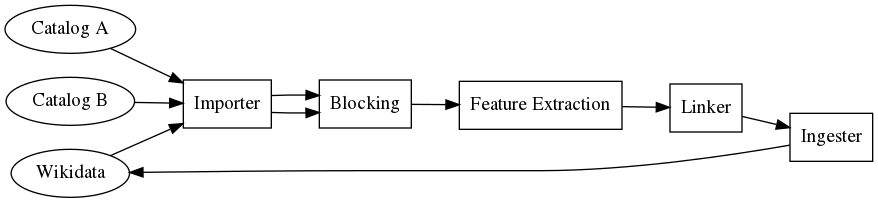
\includegraphics[width=\textwidth]{soweego_structure}
  \caption{Structure of \texttt{soweego}. \textit{Catalog A} and \textit{Catalog
      B} represent external databases which will be imported into
    \textit{Wikidata}.}
  \label{fig:soweego-structure}
\end{figure}

A section will be dedicated to each step, but just to give an overview, below is brief description of each one. To clarify the figure above, the \textit{Workflow} is a module which contains functionality for data cleaning and feature extraction. And the \textit{linker} is a module which contains functionality for blocking, the \textit{workflow}, and \textit{train, link, evaluate}.

\begin{enumerate}
\item \texttt{Importer}: 
reads the data from both the external databases (target catalogs) and Wikidata (source catalog),

\item \texttt{Blocking}: 
takes the preprocessed data and clusters each source entity on the Wikidata catalog with potential matches in the target catalogs.

\item \texttt{DataCleaning}: 
Takes the pairs of potential matches and cleans them (the \textit{Data Preprocessing} step in the record linkage workflow).
  
\item \texttt{Feature extractor}: 
takes the cleaned pairs from \textit{DataCleaning} and extracts a number of features, as previously defined in \autoref{sec:rl-workflow-feat-extraction}.
 
\item \texttt{Train, Evaluate}:
train or evaluate the performance of a machine learning algorithm given the features extracted in the previous step.

\item \texttt{Link}:
uses a previously trained machine learning algorithm to predict the final labels on some classification data. These predictions are done on features extracted from said data.
 
\item \texttt{Ingester}: 
is in charge of taking the predicted matches and uploading the confident predictions (those above a threshold) to Wikidata, while potential matches are uploaded to the \texttt{Mix'n'match}\footurl{https://tools.wmflabs.org/mix-n-match} platform to be reviewed manually by the community.
\end{enumerate}

The current work will be mainly centered around the development of the \texttt{linker} modules, and small parts of the \texttt{importer}. Although for the discussion of results  (\autoref{chap:results}) only the results of  \texttt{evaluate} and \texttt{link} module will be evaluated.  The remaining modules were developed by the rest of the team working on \texttt{soweego}\footurl{https://github.com/Wikidata/soweego/}.


\subsection{Importer}
\label{sec:soweego-st-importer}

The importer is the first step in the pipeline, and is also the one that is in charge of taking an external source of data (for example, a \texttt{csv} file), and then interpreting it, and saving the results to \texttt{soweego}'s internal database so that it can be easily consumed by the following steps.

The importer is composed of one \textit{adapter} for each external catalog. The adapter basically is the \textit{importer} for a specific catalog and is in charge of downloading the latest available dump for the catalog. 


Once this is done the adapter reads the obtained data and prepossesses it, so that it can be imported into the database. The adapter is necessary because the database dump from each catalog contains different fields, in different formats which need to be converted to a common representation. 


After cleaning, the data is then saved into the database. An important thing to note is that all of the dumps include the ID of each entity in the catalog's database, this is what will then be used as the \textit{target id (TID)}: the id of the target entities used during the  record linkage process.

The importer also defines a series of ORM database \textit{models} \cite{sqlalchemy}, which are specific to each catalog, one for each concrete entity type. For example, the importer defines an \texttt{ImdbWriter} database model which stands for entities of type \textit{writer} which come from the \textit{IMDb} catalog.

Using this modular design, allows to add new external catalogs to \texttt{soweego} without much complexity.


\subsubsection{Importing data from Wikidata}
\label{sec:importing-from-wikidata}

There is a special importer for downloading data from Wikidata. This Wikidata importer is in charge of downloading both the training and classification sets. These may then be used, together with the respective training or classification sets from an external catalog, to train a machine learning model or to classify the data using a previously trained mode.

These data sets are downloaded separately for each combination of catalog-entity. They will be used as the \textit{source catalogs} during the record linkage process.

Following is an overview of the procedure used in each case. 

\begin{description}
\item[Downloading training set:] 

To download the Wikidata training set what needs to be done is to receive the \textit{QID} of the catalog and of the type of entity. This is achieved by asking Wikidata, via a \textit{SPARQL} query, to provide all the items it has which are of the specified entity type\footnote{for example, all items which are \textit{directors}} and which also have a \textit{statement} linking them to the given target catalog identifier. 

These identifier statements can be easily used to check which of the items provided by Wikidata have also been included in the catalog's dump. 

The intersection, those with the same \textit{target id}, between this data and the data that resides in the project’s database for the specific catalog-entity defines the labeled data  for said entity that can be used for training and evaluation.
 
 
\item[Downloading classification set:] The classification set is also downloaded on a per \textit{catalog-entity} basis. The procedure for downloading it is very similar to that already mentioned above. 

The difference is that now Wikidata is asked to only send  the data regarding items of a specific entity type (for example, all \textit{Musicians}), and that are not already linked with the specified catalog.
\end{description}



\subsection{Blocking}
\label{sec:soweego-st-blocking}

When performing the \textit{blocking} procedure, \soweego compares the entities by using the \textit{name\_tokens} field. This field get created during the \textit{import} process. It consists of a list of all parts of the name of the entity. For example, the name \textit{Bernie Stewart} is composed of the parts \textit{Bernie} and \textit{Stewart}.

When performing blocking, the first thing that need to be done is to receive a Wikidata set, and the concrete entity type for which \texttt{soweego} is currently running. Then, for every entity in the Wikidata set, the blocking is made by getting all entities in the external catalog which share \textit{name tokens} with the Wikidata entity. 

To prevent getting too many results it is allowed for only a maximum of 10 external entities to be retrieved for each Wikidata entity.

For example, suppose a Wikidata entity is  currently processed, and in it's \textit{name\_tokens} field it has the following list of tokens: \texttt{[George, Hamilton]}, and suppose that the external catalog dataset for said entity is as follows:

\begin{table}[H]
\centering
\begin{tabular}{l|l}
name\_tokens        & TID   \\ \hline
{[George, Thut]}      & m3289 \\
{[Natalie, Hamilton]} & m2390 \\
{[George, Hamilton]}  & m9942 \\
{[Lucy, Waters]}      & n5932
\end{tabular}
\caption{Blocking example external catalog}
\label{tab:soweego-blocking-ex}
\end{table}

After blocking with the rule mentioned above, its possible to find that the Wikidata entity may be a possible match with \texttt{[m3289, m2390, and m9932]}, but is not a match with \texttt{n5932}.

The main reason this blocking rule was chosen, is because all entities have a name field from which the tokens can be derived.  

Choosing another field (like \textit{birth date + death date}) might yield better results, but some entities do not have said field, which makes the blocking difficult. 

\subsection{Data Cleaning}
\label{sec:soweego-st-data-cleaning}

Data cleaning is a step of the \textit{workflow}, and is executed for each entity in the pairs defined during the previous \textit{blocking} step before giving these \textit{cleaned} entities to \textit{feature extraction}. 

The ways in which the entities get \textit{cleaned} is defined in depth in \autoref{sec:soweego-st-data-cleaning}. 


\subsection{Feature Extractor}
\label{sec:soweego-st-feature-ext}

An in depth description of each feature used will be given in \autoref{sec:used-features}, for the moment it will be mentioned at a high level how the \textit{feature extraction} step works in \texttt{soweego}. 

The project leverages the \texttt{Python Record Linkage Toolkit} \cite{recordlinkage-library} to extract the features. By using this framework the process gets simplified, it only needs the definition of which feature functions to use, and to which fields they should be applied. 
After this is done, the only thing that remains is feeding to the framework the pairs of potential matches as extracted during the blocking step, and it will automatically yield the extracted features for said pairs.

For example, consider that this step gets as an input the list of potential matches extracted during the previous blocking procedure. An example of such list of pairs can be: 

\begin{center}B
    \texttt{[('Q185002', 'nm0310359'), ('Q185002', 'nm2242569'), ('Q185002', 'nm0267785')]}
\end{center}

Where the first element in each pair is the QID of a Wikidata item, and the second element is the ID of the element in an external catalog (in this case, these are the IDs of entities in the IMDb catalog). Besides these pairs, there is also access to the information about each entity (its fields). 

Finally, the feature extraction procedure also defines a list of which comparison functions to apply to which fields of the source (Wikidata) and target (IMDb in this case) entities.

The feature extraction proceeds in such a way that for every pair of entities the list of comparison functions mentioned above gets applied to each them. Each one of these \textit{function applications} will generate a value which will come to be a \textit{feature} that characterizes the relationship between the two entities.

For example, consider using only one comparison function: the same modified \textit{Levenshtein} distance that was exposed in \autoref{sec:rl-workflow-feat-extraction}. Its specified that this function should be applied to the fields with the following names: \textit{[(source.name, target.name), (source.description, target.description)]}. Below is a figure which might help explain how this application happens.

\begin{figure}[H]
  \centering 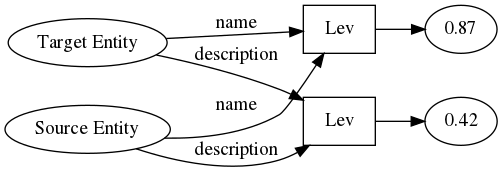
\includegraphics[width=.6\textwidth]{feature_extraction}
  \caption{Example of applying the \textit{Lev} function to a pair of entities to extract features.}
  \label{fig:feature-extractions-flow-ex}
\end{figure}

If the procedure mentioned above is applied to all the pairs in the list, in the end there should be a table where each row contains the \textit{feature vector} characterizing every pair:

\begin{table}[H]
\centering
\begin{tabular}{l|l|l}
Pair                     & Lev\_name             & Lev\_description      \\ \hline
\texttt{('Q185002', 'nm0310359')} & 0.87                  & 0.42                  \\
\texttt{('Q185002', 'nm2242569')} & 0.52                  & 0.24                  \\
\texttt{('Q185002', 'nm0267785')} & 0.74                  & 0.53                  \\
\multicolumn{1}{c}{\vdots}    & \multicolumn{1}{c}{\vdots}  & \multicolumn{1}{c}{\vdots}  
\end{tabular}
\caption{Example results of performing feature extraction using the \texttt{Lev} function, on fields \texttt{name} and \texttt{description}.}
\label{tab:soweego-feature-extraction-example-results}
\end{table}


For \texttt{soweego}, the list of functions applied may change depending on which fields are available in the target and source catalogs. For example, extracting a feature that compares the \texttt{description} of both entities only if both have said field. This means that the amount of feature vectors extracted for different concrete entities may be different. 

Once the feature vectors for all pairs become available, they may be fed to the \textit{train/evaluate/link} modules. 


\subsection{Train, Evaluate, Link}
\label{sec:soweego-st-train-evaluate-link}

These three can be treated described as one module since their functionality is very similar. The \textit{train} module trains one of the machine learning classifiers presented \autoref{chap:algorithms} on a given dataset. The \textit{evaluate} module performs the evaluation of said classifier (the evaluation step is explained more in depth in \autoref{chap:results}). And the \textit{link} module uses the trained classifier to predict whether the unlabelled pairs given by the blocking step are matches or not.

All of these modules receive their as input the matrix of feature vectors from the previous step and feeds it to one of the machine learning algorithms.

Besides this, the \textit{link} module also applies a couple of \textit{post-classification} steps on the predictions. Specifically, what it does is to apply the following \textit{linking rules} to each result in turn.

\begin{description}
\item[Wikidata URL] if the target in the corresponding pair thats currently processing has a URL, and said URL points to a Wikipedia/Wikidata page then it can automatically extract from said URL which Wikidata entity the target should be associated with. 

If this extracted entity is the same as the source entity in the pair then the probability that they match is automatically changed to 1. 

\item[Name Rule] this rule can be optionally activated when more confident results are desired, and by default is turned off. What it does is that, taking the current pair, it checks all possible fields which may be a name, and if there is no intersection among the tokenized contents of these fields then the probability of a match is decreased to 0.
\end{description}



\subsection{Ingester}
\label{sec:soweego-st-ingester}

The first step performed by the ingester is to separate the given predictions into \textit{non-matches}, \textit{potential-matches}, and \textit{confident-matches}. This is done by simply separating the predictions according to some threshold. 

For example, all predictions below 0.4 are \textit{non-matches}, above 0.4 but below 0.7 are \textit{potential-matches}, and everything above that are matches. 

The reason for this separation is because \texttt{soweego} uploads directly to Wikidata only those predictions which are very likely to be true, whilst the \textit{potential-matches} are uploaded to a service called \textit{Mix'n'match}, where the Wikidata community can check manually each proposed pair and define if it is actually a match or not.

Confident results are \textit{uploaded} by editing the relevant stamement of each Wikidata item. For examaple, if QID \textit{Q185002} is a match with IMDb TID \textit{nm0310359} then the ingester will proceed to create or update a statement on the item with the given QID, using the property \textit{P345}\footurl{https://www.wikidata.org/wiki/Property:P345} and using as a value the given TID. 

The mentioned property is used to link an item with an IMDb ID (similar properties exist in Wikidata for all the other external catalogs used).


\section{Implementation Details}
\label{sec:soweego-implementation-details}

All the development of \texttt{soweego} was made with the Python \cite{python-tutorial} programming language. To run the internal database  MariaDB\footurl{https://mariadb.com/} was used.(which is the same as that used by Wikidata, so there is minimum friction when moving the application from development to production). 
The details of communicating with the database were abstracted away with the use of \texttt{SQLAlchemy} ORM \cite{sqlalchemy}, which provides an object like interface.

To simplify the implementation of the record linkage workflow we also use the \texttt{Python Record Linkage Toolkit} \cite{recordlinkage-library} framework, which implements many useful functionalities for this goal. Mainly it eases the feature extraction and linking procedure. We also use the library \texttt{Pandas} \cite{mckinney2010_pandas} to make it easier to handle the data.

Some of the machine learning models provided were leveraged by \texttt{Scikit-Learn} \cite{scikit-learn} to be used in the linker, as well as their \textit{grid search} functionality to find the optimal hyperparameters.

All the visualizations in this work have been done by using the tools \textit{Matplotlib} \cite{Hunter_Matplotlib}, and \textit{Seaborn} \cite{Seaborn}.% not really an implementation detail

Finally, the \texttt{ML-Ensemble} \cite{flennerhag:2017mlens} framework was used to make it easier to implement the different ensemble models used.


Development of \texttt{soweego} happens locally and new releases are uploaded to a virtual private server which is provided by Wikimedia for that purpose. 


%%%%%%%%%%%%%%%%%%%%%%%%%%%%%%%%%%%%%%%%%

\chapter{Data}
\label{chap:data}

This chapter will be dedicated to showing and exploring the data that was used (next section), then mentioning which pre-processing steps the data undergoes and what it's final shape is (\autoref{sec:data-preprocessing}). Following that, the list of features extracted during the \textit{feature extraction} step of \texttt{soweego} will be discussed. Finally, a potential difference between the training and classification data is exposed in \autoref{sec:training-real-data-difference}.


\section{Original Shape of the Data}
\label{sec:orig-shape-of-data}

This section will explore which shape the data received from the external catalogs, as well as that received from Wikidata, takes. Since they are all different, a section will be dedicated to each catalog. 

It must be pointed out for the external catalogs, that even though they are maintained by a group of contributors and, in some cases, also by dedicated teams, it does not mean that the data is 100\% clean. 

During development there have been multiple encounters with malformed values (like birth or death dates in the future), spelling errors in  names, missing values (most commonly, missing birth and death dates), among others. 

As such, it must be kept in mind that the information coming from the external catalogs should not be considered the absolute truth.



\subsection{IMDb}
\label{sec:shape-imdb}

IMDb provides multiple dumps of their data\footurl{https://www.imdb.com/interfaces/}, each is a snapshot of the database up until the current date, containing different information. The one used in this project, which is the one that contains information about people in IMDb's database, is \texttt{name.basics}\footurl{https://datasets.imdbws.com/name.basics.tsv.gz}. The specific dump that is going to be discussed was downloaded from the site on \textit{3 October 2019}.

The data dump is one single tab separated file. It contains 6 different columns. An example of some rows, and explanation of each field are mentioned below.

\begin{table}[H]
\centering
\begin{tabular}{l|l|l|l|l|l}
nconst    & primaryName     & birthYear & deathYear         & primaryProfession              & knownForTitles                          \\ \hline
nm0000001 & Fred Astaire    & 1899      & 1987              & actor,miscellaneous & tt0043044,tt0053137 \\
nm0000002 & Lauren Bacall   & 1924      & 2014              & actress,soundtrack             & tt0038355,tt0071877 \\
nm0000003 & Brigitte Bardot & 1934      & \textbackslash{}N & actress,producer    & tt0054452,tt0057345
\end{tabular}
\caption{Sample of three rows from the raw IMDb data dump. The list of professions and \textit{knownForTitles} have been shortened to make the table fit. Note that IMDb uses \textbackslash{}N to symbolize a null value.}
\label{tab:imdb-raw-sample}
\end{table}

\begin{description}
\item[nconst] This is the column which holds the ID of the person in IMDb's internal database. This ID is what will later be used as the TID to identify a target entity from this catalog.

\item[primaryName] Is the full name of the person. Usually consists of a first name followed by a last name, but may include the initials of middle names as well. As will be shown later, there are even some entities which have more than 3 parts to their name.

\item[birthYear] The year in which the person was born.

\item[deathYear] The year in which the person died.

\item[primaryProfession] This field contains a comma separated list of main professions each person has, this list may contain a maximum of three professions. These \textit{professions} are names which describe the ocupation the person is known for, that is, reasons for which the person appeared in the credits of a movie or TV-series. 

These professions are not always specific, and sometimes act like clusters of similar, and more specific, professions.

\item[knownForTitles] List of movie/TV-series IDs the person is known for. This information is not currently used in our project. 
\end{description}

The interpretation of most fields is very straightforward. The only exception is the \textit{primaryProfession} field, which will be explained a bit more here. IMDb defines a series of \textit{clusters of professions}, or \textit{occupations}, which group together the accepted professions in the database. The most common professions have their own cluster (like \textit{actor}), while less common ones are clustered together (for example, \textit{music\_department} which stands for all occupations related to making music for a movie or TV-series).

The actual possible values for the \textit{primaryProfession} field are: 

\begin{quote}
    \begin{itemize*}
    \item actor
    \item actress
    \item animation\_department
    \item art\_department
    \item art\_director
    \item assistant\_director
    \item camera\_department
    \item casting\_department
    \item casting\_director
    \item cinematographer
    \item composer
    \item costume\_department
    \item costume\_designer
    \item director
    \item editor
    \item electrical\_department
    \item executive
    \item location\_management
    \item make\_up\_department
    \item manager
    \item music\_department
    \item producer
    \item production\_department
    \item production\_designer
    \item production\_manager
    \item publicist
    \item script\_department
    \item set\_decorator
    \item sound\_department
    \item soundtrack
    \item special\_effects
    \item stunts
    \item talent\_agent
    \item transportation\_department
    \item visual\_effects
    \item writer
    \end{itemize*}
\end{quote}

All the items in the this list correspond to respective professions in Wikidata, meaning its possible to later compare these with the profession associated with a Wikidata item, and from the comparison derive a feature. The mapping from these professions to Wikidata professions is explained in \autoref{sec:imdb-profs-to-wikidata}, the feature mentioned will be explained later in \autoref{sec:used-features}.

There are a total of 9,613,243 entries in the dump. Of these, all of them have some value in their \textit{primaryName} field. There are 194,469 entries which have a single word in as the name, all the other have 2 or more. In \autoref{fig:imdb-num-tokens-name-pie} its possible to see that the great majority of entities have names composed of two tokens, and the next most common amount of tokens is 3 (possibly those with a middle name), followed by those with only one token, and finally all those entities with names containing 4 or more token.

\begin{figure}[]
  \centering 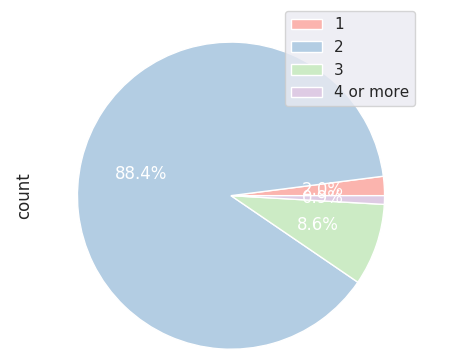
\includegraphics[width=.6\textwidth]{imdb_num_tokens_names}
  \caption{Amount of tokens in names of IMDb entities.}
  \label{fig:imdb-num-tokens-name-pie}
\end{figure}


Of all the entries, there are only 488,727 which have a \textit{birthDate}, and 170,613 have a \textit{deathDate}. The distplots in \autoref{fig:imdb-years-distplot} show the distributions of birth and death dates for IMDb. It can be noted that most of the entities were born around the 1900, and there are less entities from closer years (possibly because those individuals are still too young to have any reason to possess a page in IMDb). On the other hand, death dates behave in the inverse manner: the greatest amount of deceased entities seems to have died in the last years.

\begin{figure}[]
  \centering 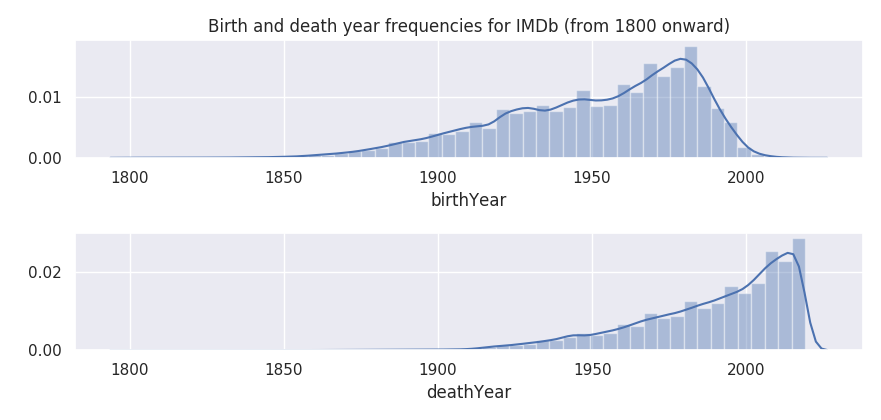
\includegraphics[width=.9\textwidth]{birth_and_death_frequencies_imdb}
  \caption{Birth (top) and death dates (bottom) for IMDb entities. Note that to generate this figure only dates later than 1800 were considered. There are 568 entities who were born earlier than 1800, and 305 entities who died before the same date. These entities are not being considered for the graphs above, in an effort to make them easier to interpret, but we do consider them during the record linkage process.}
  \label{fig:imdb-years-distplot}
\end{figure}

The professions field is quite good: only 1,881,284 don't have a profession. The remaining 7,731,959 entities either have 1, 2 or 3 professions listed. \autoref{fig:imdb-profession-count-pie} is a pie chart showing their distribution. Its possible to see that roughly $3/4$ of the entities have only one profession, and the last quarter seems to be equally shared by entities with 2 and 3 professions.

\begin{figure}[]
  \centering 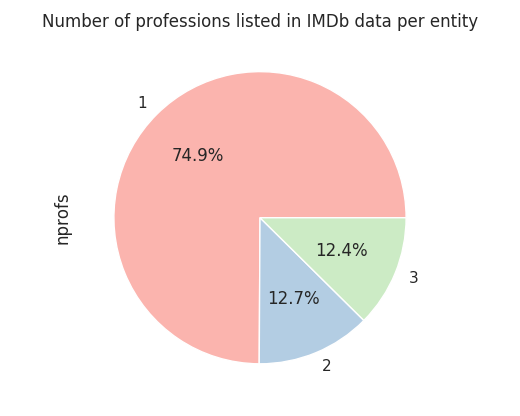
\includegraphics[width=.6\textwidth]{profession_counts_imdb}
  \caption{Counts of the number of professions listed for IMDb entities.}
  \label{fig:imdb-profession-count-pie}
\end{figure}

In \autoref{fig:imdb-profession-raw-counts} a barplot can be seen that shows the amount of times each profession appeared in the dump. And \autoref{fig:imdb-profession-single-percentage} shows the percentage of entities which only had one of the professions.

\begin{figure}[]
  \centering 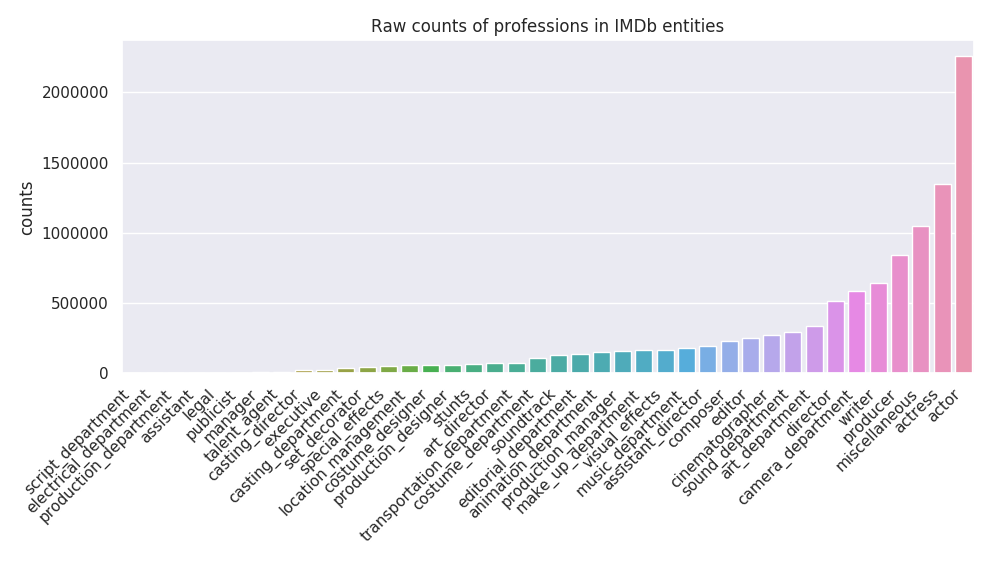
\includegraphics[width=\textwidth]{raw_profession_counts_imdb}
  \caption{Raw counts of the number of professions listed for IMDb entities.}
  \label{fig:imdb-profession-raw-counts}
\end{figure}


\begin{figure}[]
  \centering 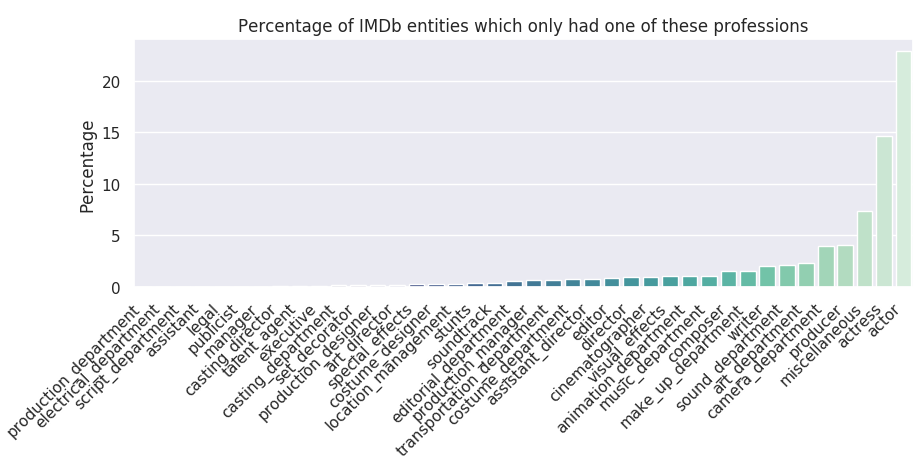
\includegraphics[width=\textwidth]{imdb_percentage_single_professions}
  \caption{Percentage of how many times each profession appeared as the single profession of an entity.}
  \label{fig:imdb-profession-single-percentage}
\end{figure}


By looking at \autoref{fig:imdb-profession-coocurrence-heatmap} a heatmap can be seen that describes the co-occurrence of the different professions (how frequent is it that an entity has them listed together in its \textit{primaryProfessions} field). Its possible to see there are some interesting correlations among them, for example, that the \textit{director} profession almost always appears together with the \textit{writer} profession. This shows that there is an underlying structure in the professions, which is another motivation to create a feature that leverages this field.

\begin{figure}[]
  \centering 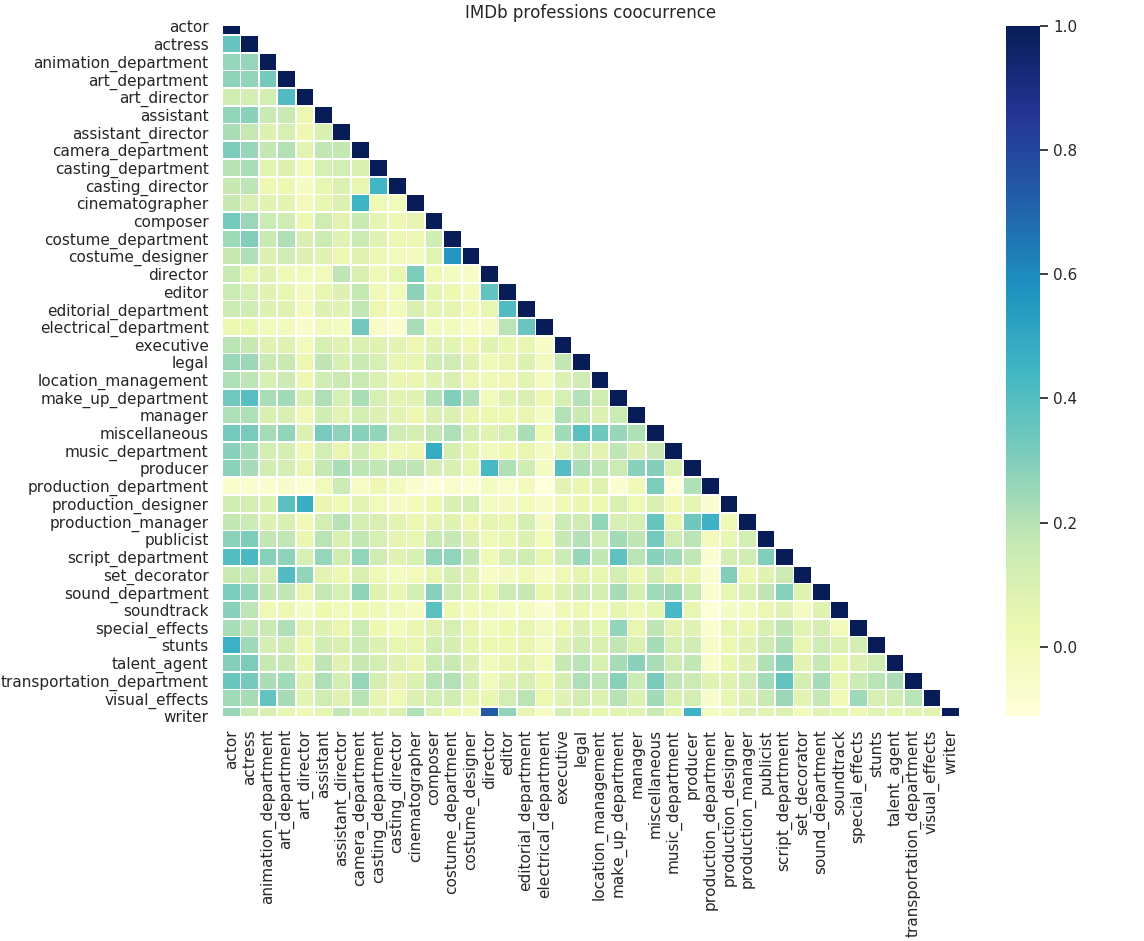
\includegraphics[width=\textwidth]{imdb_profession_coorcurrence}
  \caption{Co-occurrence of IMDb professions.}
  \label{fig:imdb-profession-coocurrence-heatmap}
\end{figure}

Its evident that the IMDb dump does not provide much information that can be used. The name fields seem to be the ones with the highest quality (no empty values). Birth and death dates are quite informative but sadly only few entities have values there. The remaining field, \textit{primaryProfessions}, is also quite good in terms of data quality, and its underlying structure will allow the creation of an effective feature from it.



\subsection{Discogs}
\label{sec:shape-discogs}

Discogs provides multiple data dumps\footurl{https://data.discogs.com/}, and maintains records of dumps released in different dates. The one used for this project is \textit{discogs\_20190901\_artists}, whose last revision was on \textit{2019-09-08T13:03:25.000Z}.

This dump contains information about artists, which can be either a single musicians or music groups. The dump is an XML file and for each entity (either band or musician) provides the following information:

\begin{description}
\item[identifier] This is the ID of the entity in the Discogs database. It will be the field used as the TID for this catalog.

\item[name] The main artistic name associated with the entity.

\item[realname] The real name of the entity, which might differ from it's artist name.

\item[namevariations] Possible different artist names for this entity.

\item[data\_quality] Discogs specific metric that shows how good the data is. It's possible values are 
\begin{itemize*}
    \item Correct
    \item Complete and Correct
    \item Needs Vote
    \item Needs Minor Changes
    \item Needs Major Changes
    \item Entirely Incorrect
\end{itemize*}

\item[profile] This is the profile description of an entity.

\item[living\_links] This field holds a list of hyperlinks associated with the entity. They are usually links that go to external sites (for example, Twitter, Wikipedia, YouTube, etc).

\item[group] This field is specified for entities which are a musician. It specifies which groups the musician belongs to. This project only considers \textit{musicians} as those who have some value in this field. This information is only used to determine which entries are \textit{musicians}, and is not otherwise leveraged in the project. 

\item[members] This field is specified for bands, and shows which musicians are associated with which bands. This project  only considers as \textit{bands} those entities which have some value in this field. This information is only used to determine which entries are \textit{bands}, and is not otherwise leveraged in the project.

\end{description}

There are a total of 6,432,264 entities in the Discogs dump. Of these, 1,129,711 have a value in either the \textit{band} or \textit{members} field. This is the final number of entities \texttt{soweego} will import into its database, so these are the ones for which all the next metrics will be derived.

There are 384,352 entities which have some value in the \textit{members} field, meaning that these are the bands in the data dump. And there are 749,499 which have a value in the \textit{groups} field (these are the musicians). There are also 4,140 entities which have \textit{both} members and groups. \autoref{fig:discogs-band-member-commonality} shows the most common number of bands a musician belongs to, and the most common number of members a band has. It can be seen that it is more common for bands to have multiple members, whilst it is not very common for a musician to be part of more than one band.

\begin{figure}[]
  \centering 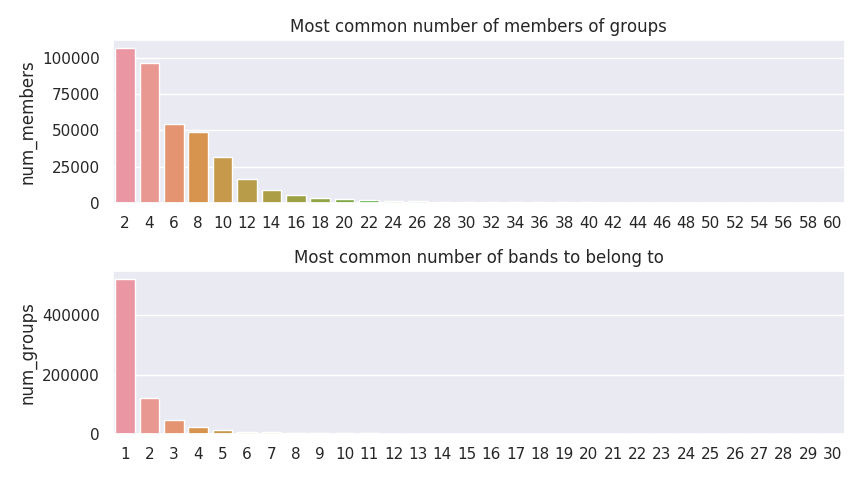
\includegraphics[width=\textwidth]{discogs_band_belonging_barplots} 
  \caption{The plots above show what is the most common number of members in a band (top) and the most common number of bands a musician belongs to.}
  \label{fig:discogs-band-member-commonality}
\end{figure}


Of all the entities, 935,456 are not associated with a real name. However, all of them do have a \textit{name}. Most of these are composed of 2 tokens. \autoref{fig:discogs-num-name-tokens-distplot} shows the distribution of the number of tokens for the names of the entities. Notice that 2 is the most common, but 3 and 4 are also quite common.

\begin{figure}[]
  \centering 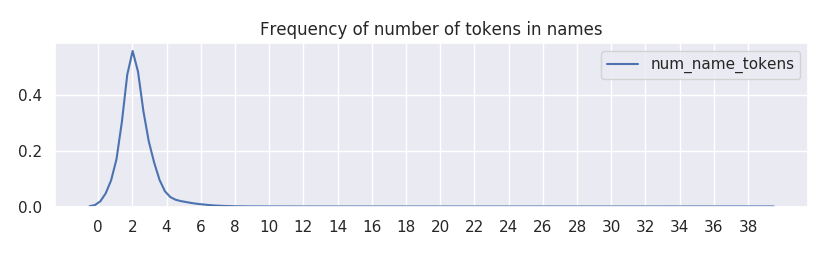
\includegraphics[width=\textwidth]{discogs_distribution_num_name_tokens} 
  \caption{Distribution of the number of tokens in names of Discogs entities.}
  \label{fig:discogs-num-name-tokens-distplot}
\end{figure}

There are 492,315 entities which have at least one value in the \textit{namevariations} field. \autoref{fig:discogs-num-name-variations-barplot} shows which are the most common number of alternative names, among entities who actually have alternative names. Notice that it is much more likely to have only one name variation, with the likelihood of having another decreasing almost by half with each extra alternative name.

\begin{figure}[]
  \centering 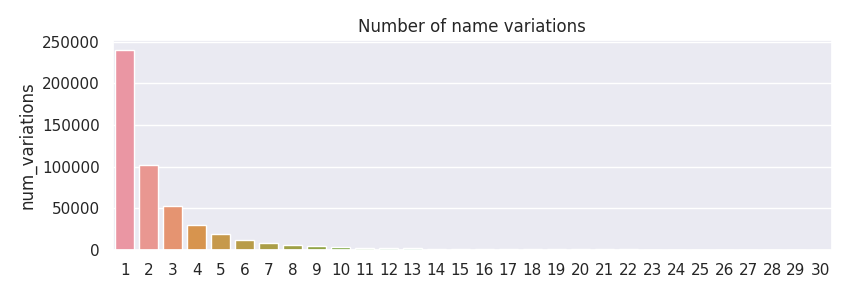
\includegraphics[width=\textwidth]{discogs_num_name_variations} 
  \caption{Distribution of the 30 most common number of tokens in names of Discogs entities.}
  \label{fig:discogs-num-name-variations-barplot}
\end{figure}


Regarding the \textit{profile} field, which comes to be like the description of the entity, 487,588 have some kind of value in it. \autoref{fig:discogs-num-words-profile-barplot} shows the distribution of how many words can be expected to be found in such description (among entities who do have one). Notice that if an entity has a profile description then the most likely scenario is that it will have one composed of only two words. It's interesting to notice that having only one word in the description is almost as likely as having 7 of them. 

\begin{figure}[]
  \centering 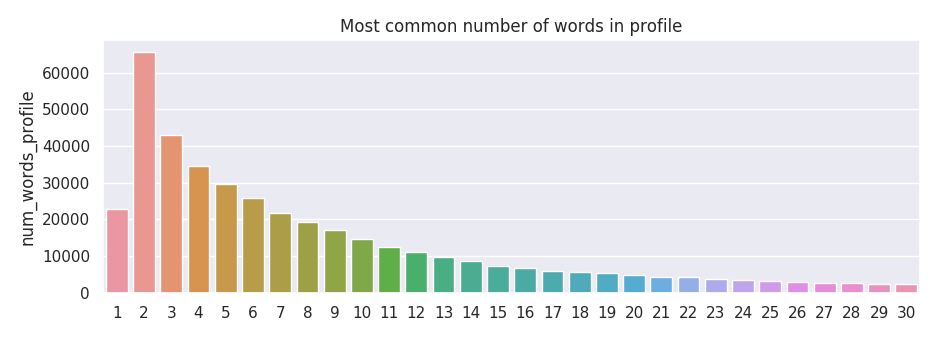
\includegraphics[width=\textwidth]{discogs_num_words_profile} 
  \caption{Distribution of the 30 most common amount of number of words in the \textit{profile} of Discogs entities.}
  \label{fig:discogs-num-words-profile-barplot}
\end{figure}


Discogs also provides how many entities are associated with links to external pages. In the dump there are 243,757 entities with external links. \autoref{fig:discogs-external-links-counts-barplot} shows which amount of links is the most common among entities which do have links. It seems to be very common, if an entity has at least one link, that it actually has only one. Entities with 3 and 4 links can be found, but 5 or more are much less common.

\begin{figure}[]
  \centering 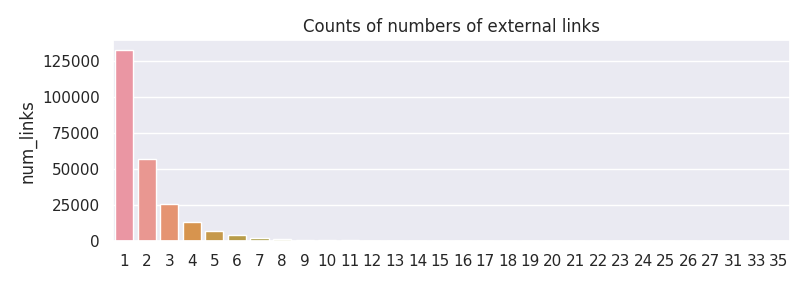
\includegraphics[width=\textwidth]{discogs_external_links_counts} 
  \caption{Distribution of the 30 most common amount of external links associated with Discogs entities.}
  \label{fig:discogs-external-links-counts-barplot}
\end{figure}

The \textit{data\_quality} field shows how good the data about a certain entity is. All entities have a value in this field. \autoref{fig:discogs-data-quality-distribution-pie} provides the distribution of the various data quality labels. Its possible to see that more than half of them are marked as \textit{Needs Vote}, little less than a quarter are \textit{Correct}, and the rest are labelled as incorrect (in different degrees).

\begin{figure}[]
  \centering 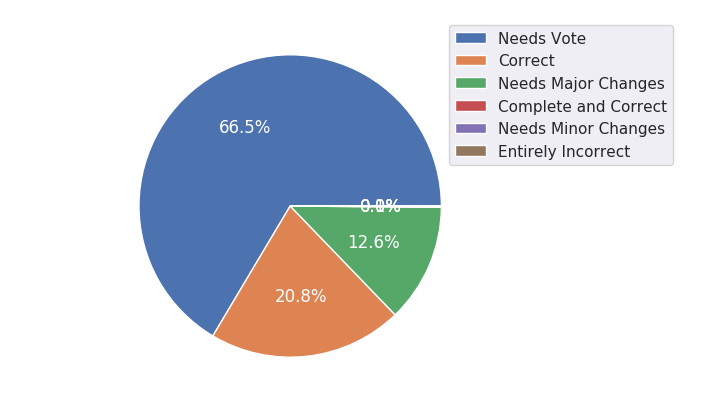
\includegraphics[width=\textwidth]{discogs_data_quality_distribution} 
  \caption{Percentages of entities marked with a given \textit{data quality} label.}
  \label{fig:discogs-data-quality-distribution-pie}
\end{figure}


\subsection{Musicbrainz}
\label{sec:shape-musicbrainz}

The Musicbrainz dump\footurl{https://musicbrainz.org/doc/MusicBrainz_Database/Download} is a snapshot of the whole dataset. As such, it contains a lot of data which is not of any interest for this project. The dump used for this catalog is the following:

\begin{itemize}
    \item 20191002-001702/mbdump.tar.bz2
\end{itemize}

In the dump there are a total of 1,003,366 musicians and 437,287 bands. The dump provides the following information about each of these entities:

\begin{description}
\item[gid] The id of the entity in Musicbrainz's database. This is the ID that will be used as the TID during the record linkage procedure. 

\item[name] Name of the entity.

\item[birth day, birth month, birth year] Define individually which is the day, month, and year a person was born in. If one of these is unknown then the value is \textit{NULL}. By having this separate, the \textit{precision} with which a date is known can be derived. This will be useful later when deriving features from said dates. 

\item[death day, death month, death year] Same as the fields mentioned above, but for death dates.

\item[birth place, death place] Specify information on where the person was born, and/or died. For bands, the birth and death dates symbolyze where the band was formed and where it separated.

\item[gender] Specifies the gender of the entity (\textit{male} / \textit{female}).

\item[type\_id] This field specifies which type is the entity in question. Possible values are: \textit{person}, \textit{character}, \textit{orchestra}, \textit{choir}, \textit{group}. Entities with any of the first two values are considered \textit{musicians}, whilst those with any of the last three are considered \textit{bands}.

\item[links] The external links an entity is associated with.

\item[relations with bands] It specifies the relation among artists and bands, specifically, the list of bands to which they belong. 
\end{description}

All entities have a name associated to them. \autoref{fig:musicbrainz-name-tokens-pie} shows the distributions for said number of tokens. It is interesting to note that bands are almost as likely to have a name composed by a single token than they are to have one with two. Another interesting thing is that names of bands are more likely than those of people to contain more than two tokens.

\begin{figure}[]
  \centering 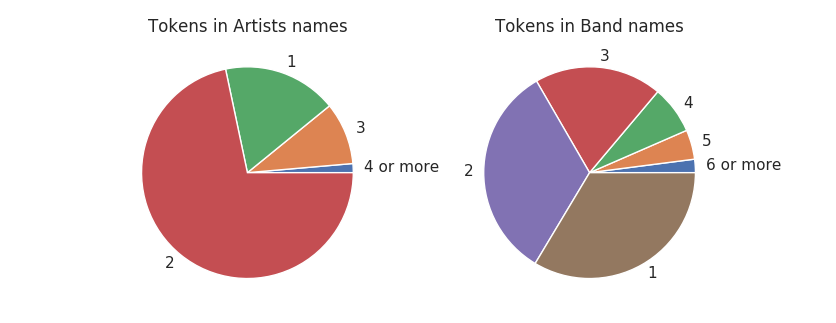
\includegraphics[width=\textwidth]{musicbrainz_token_names_entities} 
  \caption{Percentage of entities which have a name composed of a specific number of tokens.}
  \label{fig:musicbrainz-name-tokens-pie}
\end{figure}

As per gender distribution, there are much more \textit{males} than \textit{females}. There are 767,616 musicians for which the gender is specified. This distribution is shown in \autoref{fig:musicbrainz-gender-pie}. Notice that less than a quarter of entities are \textit{female}.

\begin{figure}[]
  \centering 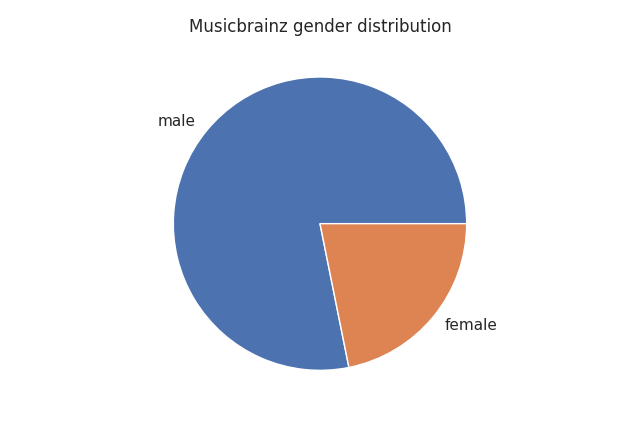
\includegraphics[width=.8\textwidth]{musicbrainz_gender_pieplot} 
  \caption{Percentage of entities separated by gender.}
  \label{fig:musicbrainz-gender-pie}
\end{figure}


There are 297,011 musicians and 164,060 bands which are associated with a birth date. There are also 88,191 musicians and 34,213 bands who have a death date defined. The distribution of the frequency of said dates can be seen in \autoref{fig:musicbrainz-dates-distplot}. Notice how the curve symbolizing the birth date of musicians is much more smooth than that of groups, and there seems to have been a peak in the amount of groups created in the latest years. This suggests the adaptation of this digital platform is more common for the newer generation of bands. Also death years seem to follow this same behaviour.

\begin{figure}[]
  \centering 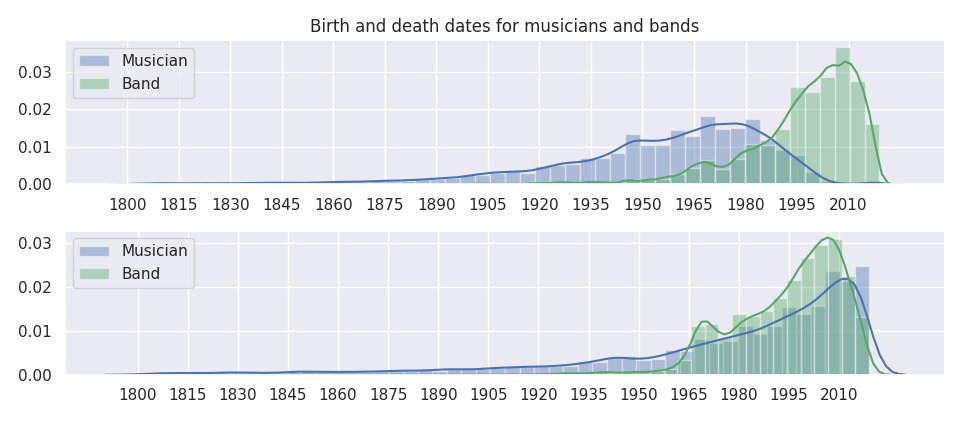
\includegraphics[width=\textwidth]{musicbrainz_birth_death_dates_distplot} 
  \caption{Distribution plot of the years musicians were born or died; and years in which bands were created or dissolved. Top shows the distribution of birth/creation years, while bottom shows the \textit{death}/\textit{dissolve} years. Dates for musicians are in \textit{blue}, and those for and bands are \textit{green}. Note that both graphs were created by considering dates later than \textit{1800} and earlier than \textit{2020} (which at the time of this writing is in the future). However, dates outside this range, were used during the performance of record linkage.}
  \label{fig:musicbrainz-dates-distplot}
\end{figure}

There are 223,340 musicians and 94,826 bands associated with a birth place. Similarly there are 53,631 musicians and 4,885 bands associated with a death place. These behave similarly as the birth and death dates, where there are more entries with birth date than death date.

There are 517,524 musicians and 266,206 bands which are associated with at least one external link. \autoref{fig:musicbrainz-links-number-pie} shows which percentage of musicians or bands have a certain number of links. It can be seen that both more commonly than not have only one link. However, it is more common for bands to have more links than musicians. 

\begin{figure}[]
  \centering 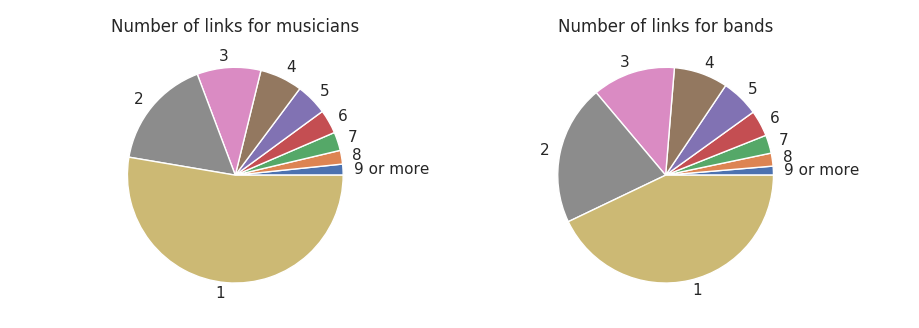
\includegraphics[width=\textwidth]{musicbrainz_number_of_links_musician_band} 
  \caption{Distributions of the number of external links for musicians and for bands.}
  \label{fig:musicbrainz-links-number-pie}
\end{figure}


\subsection{Wikidata}
\label{sec:shape-wikidata}

% mention for each catalog, and which entities it has. Potentially mention the
% number of entities for each type of entity.

For Wikidata we download training and classification \textit{sets}, one pair for each concrete entity. As explained in \autoref{sec:importing-from-wikidata}, the training data already contains the labels, or true links, for each entity, and is what is used to train the different machine learning algorithms. This basically means that each Wikidata \textit{training} dump has a field named \textit{TID}, which is the ID of the target catalog. On the other hand, the classification data are the entities that don't have target identifiers and need to be linked. This data is downloaded through Wikidatas public SPARQL endpoint,\footurl{https://www.wikidata.org/wiki/Wikidata:SPARQL_query_service} which allows us to easily get the relevant statements about a given entity.

Following are the fields that we gather from Wikidata. Note that, as said above, \textit{TID} only appears in \textit{training} set. 

\begin{description}

\item[TID] ID of the entity in a specific external catalog. Only found in the dumps used for training. The actual values may change depending on which catalog this dump was downloaded for. For example: if the dump was downloaded to be used with IMDb, then the TIDs are reference to IMDb entities. If it was downloaded for Discogs, then the TID will reference Discogs entities. 

\item[QID] This is the unique identifier of the Wikidata entity. This is what will be used as the \textit{source ID} while performing record linkage. Note that in the present work the terms \textit{QID} and \textit{source ID} will be used interchangeably.

\item[name] The name of the entity in Wikidata.

\item[url] List of URLs associated with the entity. These are URLs about the entity, and may point to Wikidata pages in other languages, or external catalogs.

\item[description] The description of the entity in Wikidata.

\item[born] Specifies the date the entity was born.

\item[died] Specifies the date the entity died.

\item[sex\_or\_gender] Specifies the gender of the entity.

\item[place\_of\_birth] Specifies the entity was born.

\item[place\_of\_death] Specifies the place where the entity died.

\item[pseudonym] Is a list of alternative names by which the entity might be known.

\item[occupation] List of QIDs representing the professions an entity is known to have performed.

\item[birth\_name] The name of the entity, given at birth.

\item[given\_name] The first name or forename of the entity.

\item[family\_name] The last name or surname of the entity.
\end{description}

\autoref{tab:wikidata-dumps-sizes} shows which is the size of the datasets, both the training and classification ones, for each concrete entity. It seems that the datasets for both musicians are among the largest in both cases, in fact they are except for the \textit{IMDb Actor} training set, which is the largest by a bit more than $50k$. On the other hand, the smallest classification set is \textit{IMDb Producer}, by almost $20k$. In the classification sets, the ones for IMDb \textit{producer} and \textit{director} are much tinier in comparison than all the other. 

\begin{table}[H]
\centering
\begin{tabular}{l|l|l|l}
\textbf{Catalog}     & \textbf{Entity}   & \textbf{Number of Entities Train} & \textbf{Number of Entities Classification} \\ \hline
Discogs     & Band     & 43,428                   & 36,200                            \\ \hline
Discogs     & Musician & 88,069                   & 183,483                           \\ \hline
IMDb        & Actor    & 177,417                  & 89,081                            \\ \hline
IMDb        & Director & 46,904                   & 8,407                             \\ \hline
IMDb        & Musician & 61,034                   & 210,017                           \\ \hline
IMDb        & Producer & 19,861                   & 2,075                             \\ \hline
IMDb        & Writer   & 41,373                   & 15,143                            \\ \hline
Musicbrainz & Band     & 47,096                   & 32,407                            \\ \hline
Musicbrainz & Musician & 118,107                  & 153,437                           \\ \hline
\end{tabular}
\caption{Sizes of Wikidata dumps for training and classification.}
\label{tab:wikidata-dumps-sizes}
\end{table}



\section{Preprocessing}
\label{sec:data-preprocessing}

This section will show which steps the raw data undergoes before it can be used in the \textit{feature extraction} steps. There are actually two different preprocessing steps, one for data coming from Wikidata, and another for data coming from external catalogs. There are also some steps which are applied to data coming from both sources. That is why this section will be separated into three subsections, one explaining each set of steps. During the importing process, the raw dump of the external catalogs also gets briefly preprocessed, these modifications will me mentioned in the last subsection.

It is important to note that the preprocessing for \textit{Wikidata} or \textit{External} data happen before the \textit{Shared} preprocessing. 

All of this preprocessing steps, except for those in made in the \textit{importer}, are done when the data is loaded from the database.

In the cases of \textit{Shared}, \textit{Wikidata}, and \textit{External} preprocessing, it is done for chunks of data at a time, currently 1000. The \textit{Importer} preprocessing, on the other hand, is done for each entity separately. 


\subsection{Shared Preprocessing}
\label{sec:data-preprocessing-shared}

\subsubsection{Normalize dates}
\label{sec:data-preprocessiong-date-normalization}

The dates are by default saved together with their precision. The precision is a number which signals which is the most specific part of the date that it can confidently be said is correct. Especially for data coming from Wikidata, this precision can be anything from knowing the exact second something happened, to knowing in which range of one billion years it happened\footurl{https://www.wikidata.org/wiki/Special:ListDatatypes}.

For the current application, it is important that for all dates it is known at least the year. For instance, the worst precision, which is is any number $\leq 9$, will be converted to a precision of 9, which indicates that at most the year can be trusted. A precision of ten indicates that both the the month and year are known. A precision of 11 or more indicates that the year, month, and day are known. And so on until a precision of 14, which indicates that everything up to the second is known. 

This date normalization what it does is convert the dates to \textit{Pandas} \cite{mckinney2010_pandas} \textit{Period} objects, which can contain the precision of the date internally. 

This procedure is performed for both birth and death dates 

\subsubsection{Normalize names}
\label{sec:data-preprocessiong-name-normalization}

This step normalizes all possible \textit{name fields}, which are: 

\begin{itemize}
    \item name
    \item alias
    \item birth name
    \item family name
    \item given name
    \item pseudonym
    \item real name
\end{itemize}

Any of these fields can contain a list of possible names for an entity. The way in which they're actually normalized is by performing the following steps on each possible name:

\begin{enumerate}
    \item Remove any white space padding which the name may have on the left or right.
    
    \item Normalize all characters to the \textit{ascii} alphabet. This means removing the \textit{accent} from characters, and converting characters in other alphabets (e.g. Cyrillic) to \textit{ascii} characters.

    \item Make the name lowercase.
\end{enumerate}

\subsubsection{Normalize occupations}
\label{sec:data-preprocessiong-occupations-normalization}

This step simply takes the list of all occupations an entity has and converts them to a set (i.e. removes the duplicates). It also removes \textit{empty occupations}. If the occupations are not already a list then they get converted to one before the list is converted to a set.


\subsection{Wikidata Preprocessing}
\label{sec:data-preprocessing-wikidata}

\subsubsection{Drop columns with empty values}
\label{sec:data-preprocessiong-wik-drop-empty}

As the name of this step implies, what is done is that all columns in the entity which are composed of only \textit{null} values are removed. 

\subsubsection{Ensure one target ID per QID}
\label{sec:data-preprocessiong-name-one-tid}

This step is exclusively applied to Wikidata entities that come from a training dump. It ensures that all QIDs in the positive samples of the training data are only associated with one TID. This is done by checking all QIDs which are associate with more than one TID, all associations besides the first one are dropped. 

\subsubsection{Tokenize names}
\label{sec:data-preprocessiong-wik-name-tokenization}

This step is applied to all \textit{name} fields, which were defined earlier in the shared \hyperref[sec:data-preprocessiong-name-normalization]{\textit{Normalize names}} step. In fact, this step performs the same normalization on the names as the previously mentioned step. But in addition to that it also tokenizes the resulting normalized names. 

This is done by splitting the resulting normalized names on the white space that separates each part of the name, and then removing from this list of \textit{name parts} all those which are considered \textit{stopwords} according to a previously defined list. Finally this filtered list is converted to a set so that it only contains unique \textit{tokens}. 

If an entity has more than one name in a given name field then the tokens coming from all names are added to the set mentioned above. 

\subsubsection{Tokenize URLs}
\label{sec:data-preprocessiong-wik-URL-tokenization}

Each URL is first separated into the following five components:

$$
\text{<scheme>://<netloc>/<path>?<query>\#<fragment>}
$$

Then the \textit{netloc} is further splitted into tokens, where each token is each word in the string, these are called \textit{domain tokens}. From these \textit{domain tokens}, common top level domains (\textit{com}, \textit{org}, \textit{net}, \textit{info}, \textit{fm}), as well as domain prefixes (\textit{www}, \textit{m}, \textit{mobile}) are removed. 

Following this, the \textit{path} is splitted into its respective chunks, by splitting on the slash (/) character. The words in these chunks are extracted, and these are then added via \textit{union} to the set of tokens coming from the domain. 

Finally, the \textit{query} is split into its constituent words and these are also added via \textit{union} as part of the tokens from the \textit{domain} and \textit{path}. 


% Not describing this since it is not used by "people/bands"
% \subsubsection{Tokenize genres}
% \label{sec:data-preprocessiong-URL-tokenization}


\subsection{External Data Preprocessing}
\label{sec:data-preprocessing-external}

\subsubsection{Drop columns with empty values}
\label{sec:data-preprocessiong-ext-drop-empty}
% note, there is a section with the same name for wikidata

This step is the same as what is done for Wikidata. Columns which are entirely composed of \textit{null} values are dropped.

\subsubsection{Pair dates with precision}
\label{sec:data-preprocessiong-ext-date-precision}

The step is executed once for birth dates and another for death dated. It simply takes the value of the date, and the precision for said date, and joins them in a tuple. The reason for this is that then this tuple can be given to the shared \hyperref[sec:data-preprocessiong-date-normalization]{\textit{Normalize dates}} step, which will extract the appropriate Pandas Period objects.

After joining the precision and dates, the precision column is eventually dropped from the data set. 

\subsubsection{Aggregate data on target ID}
\label{sec:data-preprocessiong-ext-aggregate-tid}

If the data currently being processed contains more than one row for some TID then the values of these rows are joined together by performing a \textit{set union} on the values of each field. For example, say that the table below is the input data:

\begin{table}[H]
\centering
\begin{tabular}{l|l|l}
TID  & Name               & Zip Code    \\ \hline
\textbf{6567} & {[}Gary, George{]} & {[}93124{]} \\
\textbf{6567} & {[}George, Paul{]} & None       \\
3251 & {[}John{]} &    None    

\end{tabular}
\end{table}

There are two entries with the TID \textit{6567}. If they are then aggregated using \textit{set union} as mentioned above, the output will look like the following table:

\begin{table}[H]
\centering
\begin{tabular}{l|l|l}
TID  & Name                     & Zip Code    \\ \hline
\textbf{6567} & {[}Gary, George, Paul{]} & {[}93124{]} \\
3251 & {[}John{]} &    None    
\end{tabular}
\end{table}

Note that now the information of both rows with TID \textit{6567} have been joined into the same row.


\subsection{Preprocessing During Import}
\label{sec:data-preprocessing-import}

The following steps are applied on the raw catalog dump data while it is being imported into \soweego's internal database. Said preprocessing steps are:

\begin{enumerate}
    \item \texttt{Tokenize names} -- this is done in the same way as is done for Wikidata, explained in \autoref{sec:data-preprocessiong-wik-name-tokenization}.
    
    \item \texttt{Tokenize URLs} -- also the same as done for Wikidata, explained in \autoref{sec:data-preprocessiong-wik-URL-tokenization}.
    
    \item \texttt{Tokenize description} -- this step essentially the same as the \textit{Tokenize names} one. The difference is that here the tokenization is done on the \textit{description} field instead of the \textit{name}.
\end{enumerate}



%%%%%%%%%%%%%%%%

\section{Features}
\label{sec:used-features}

This section will be centered around explaining said list of functions, and on what fields they're applied. Each feature will be explained in depth in it's own subsection.

Note that not all features get extracted every time: they're only applied if possible. For example, if we have a feature function which needs to compare URLs, it will only be used if both entities have URLs to compare. \texttt{soweego} automatically checks that entities have the fields a feature function depends on before applying it.


\subsection{Exact match on names}
\label{sec:feature-exact-match-names}

This feature is extracted by taking the \textit{name} fields of both entities and checking if they're the same. This field may have more than one value (e.g., in the case of name variations), so the feature compares all possible pairs of names, and optimistically yields \textit{1} if any of the comparisons is a match. Remember that the values of features may go from \textit{0} (not a match), to \textit{1} (perfect match). 

For clarification, below is the algorithm used to find the perfect match. Note that this same procedure can be applied when performing \textit{perfect match} on any two lists of values.

\begin{lstlisting}
def exact_match_name(source_entity, target_entity):
    for source_name in source_entity.names:
        for target_name in target_entity.names:
            if source_name == target_name:
                return 1
    return 0
\end{lstlisting}

\subsection{Exact match on URLs}
\label{sec:feature-exact-match-urls}

Similarly to the feature defined above, both source and target entities may have a list of URLs associated with them. The returned feature will be \textit{1} if any pair of URLs is exactly the same, and 0 otherwise.

\subsection{Shared tokens in URLs}
\label{sec:feature-shared-tokens-plus-urls}

This feature expects that both entities that are being compared have a list of URL tokens (which were extracted during the preprocessing step: \autoref{sec:data-preprocessiong-URL-tokenization}). Besides this, it also receives a set of stop words $\beta$, which are words that shouldn't be considered during the comparison process.

This function takes all the URL tokens for each entity $i$ and converts them to a set, so there are two sets $\alpha$ which contain all URL tokens for a specific entity. All stop words are then removed from these sets $\sigma = \alpha
\setminus \beta$. Finally the final score is calculated as follows:

\begin{equation*}
    \frac{
        min(\|\sigma_{source}\|, \|\sigma_{target}\|)}
        {\|\sigma_{source} \cap \sigma_{target}\|}
\end{equation*}

Basically, this function measures the percentage of elements of the smallest set which are shared among both sets of tokens. If the smallest set is composed of only one element and this element is also in the largest sent then the value of this feature will be \textit{1}. If on the other hand the value is not contained in the largest set then the value will be \textit{0}.

Using a set of stop words greatly diminishes the amount of times the function classifies as similar URLs which are not really similar. This set of stop words was constructed by taking all URL tokens in the database, counting them, and choosing the most common 850. Terms in this set are mainly domains to common websites like \textit{Facebook}, \textit{YouTube}, etc, as well as common words and names.

\todo[inline,backgroundcolor=blue!25]{if time: add graphics relating urls and stopwords}

\subsection{Similar Birth Dates}
\label{sec:feature-similar-birth-dates}
 
 This function compares a pair of dates by comparing only the parts that are certainly correct. For example, remember that in \autoref{sec:shape-musicbrainz} it was said that for \textit{Musicbrainz} we separately get the value of the birth year, month, and day, and that some or all of these may not be specified. IMDb specifies only the year, and Discogs does not provide us with birth nor death dates at all. 
 
 This means that dates coming from \textit{Musicbrainz} have a variable precision, depending on what was specified in for the entity in the dump file, but the highest possible precision to know all three of these. For IMDb, on the other hand, only the year of the dates can be assumed to be correct.
 
 The \textit{date precision} specifies which parts of the dates can be trusted. It goes from less specific to more specific. For example the most general a precision can be is to have only the year as the trusted part of the date. The next, more specific step, is to trust the month, followed by the day, etc.
 
This feature function supposes that the entities have a birth date $\delta_i$, and also have a specified precision $\phi_i$ for said date. A date has at most 3 parts (year, month, and day), and as such also has a maximum precision of 3, since the most precise part of the date is the day. A given pair of dates can only be compared up to the lowest common precision, this is just $min(\phi_{target}, \phi_{source})$. 

The comparison can start from the lowest precision and keeping a counter $\omega$ to see how many parts of the dates are the same. If after comparing the lowest precision part (the year) yields that they're the same then the counter is increased and the next, most specific part, can be compared. The process is stopped when the maximum precision is reached (\textit{day}) or when the parts currently being compared are not equal.

More formally, the following pseudocode defines the algorithm:

\begin{lstlisting}
shared_precision = min((*$\phi_{target}, \phi_{source}$*)) # the maximum precision we can compare
(*$\omega$*) = 0 # counter to track how many parts the dates have in common

for date_part in 0..shared_precision:

    # get the part corresponding to the current precision, starting from the 
    # lowest, which is the year
    source_part (*$\leftarrow$*) (*$\delta_{source}$*)[date_part]
    target_part (*$\leftarrow$*) (*$\delta_{target}$*)[date_part]
    
    if source_part == target_part:
        (*$\omega$*) += 1
    else:
        break
\end{lstlisting}

Finally, the feature is then calculated as follows.

\begin{align*} 
\frac{\omega}{\text{max\_precision} + 1}
\end{align*}

Basically, this is just the percentage of sequential parts that are the same among all parts that can be compared. The lowest precision, \textit{year}, corresponds to a precision of \textit{0}, that is why we add the $+1$ in the denominator.

For IMDb dates this function just compares the years, and if they're the same then returns \textit{1}, or \textit{0} if they are different. For \textit{Musicbrainz}, which has more \textit{flexible} dates, this function is much more useful, since it allows the comparison with arbitrary precision values.
 
Note that if entities have more than one birth date then all the possible pairs are compared and the best result is returned.  
 
\subsection{Similar Death Dates}
\label{sec:feature-similar-death-dates}
 
This feature is exactly the same as the one shown above for birth dates, but is applied to death dates instead.

\subsection{Levenshtein distance on name tokens}
\label{sec:feature-levenshtein-on-name-tokens}

Levenshtein distance \cite{levenshtein1966binary} is a string comparison metric which measures how different two given strings are by considering how many insertions, deletions, and updates need to be made to make both strings equal. Below is the representation\footnote{Adapted from \url{https://en.wikipedia.org/wiki/Levenshtein_distance}} of the Levenshtein distance as a dynamic programming algorithm:

\begin{equation*}
  lev_{a,b}(i,j) =
  \begin{cases}
    max(i, j), & \text{if}\ min(i,j) = 0  \\
    min   
    \begin{cases}
        lev_{a,b}(i-1,j) + 1  \\
        lev_{a,b}(i,j-1) + 1  \\
        lev_{a,b}(i-1,j-1) + 1 * (a_i \neq b_j)  
    \end{cases} & \text{otherwise}
  \end{cases}
\end{equation*}

Where $a$ and $b$ are the strings that are currently being compared. $i$ and $j$ are the indices of the characters currently being compared. Initially the process starts from the end of the strings, so $i = |a|$ and $j=|b|$. In the original formulation, the strings are \textit{1-indexed} (\textit{0} means the string has been completely processed). $lev_{a,b}(i,j)$ stands for the distance between the first $i$ characters of $a$, and the $j$ characters of $b$. 

The calculation of the distance starts by checking if either of $i$ or $j$ are 0. If they are, then the number of changes needed is the same as the number of characters still remaining in the longest string (which are the number of characters that need to be inserted into the shortest one). 

If on the other hand none of $i,j$ are 0, then the function is recursively applied to all possible variations (in the $min$ branch), and the minimum among them is returned. The first variation corresponds to deleting a character from $a$. The second corresponds to inserting a value in $a$. Finally, the thirst stands for a replacement.

Note the $+1$ at the end of all variations. These are the penalty paid each time one of these branches needs to be taken. In the third variation, the penalty is only applied of the characters at positions $i$ and $j$ are different (i.e. there is need to perform an update). If the strings are the same then this third branch will be taken for every character comparison, and the penalty will always be \textit{0}.

The resulting score increases the more \textit{dissimilar} two strings are. However, since feature functions need to return 0 when dissimilar and 1 when similar, the result of the Levenshtein function is adapted in the following way:

\begin{equation*}
    \frac{Lev(a,b)}{max(|a|,|b|)}
\end{equation*}

If the two strings being compared are completely different then every character of the shortest string must be changed, and extra characters need to be inserted to make it equal to the longest string. These changes sum up to maximum string length. In this case, the division would yield \textit{1}, effectively signaling that the strings are completely different. 

If the entities have more than one set of name tokens (i.e. they have multiple names associated with them, which have all been tokenized) then the function shown above is applied to all possible combinations and the best result is returned. Note that before comparison, each list of tokens (which corresponds to only one name) is joined into a single string.

\subsection{Cosine similarity on name tokens}
\label{sec:feature-kernel-similarity-name-tokens}

Cosine similarity has long been used in the field of information retrieval \cite{singhal_modern_information_retrieval} since it allows to measure the distance between two \textit{documents} by checking which words they have in common. This behaviour is similar to what the current function should to, the difference is that instead of names we want to count the occurrence of \textit{bi-grams}. 

More in general, $n$-grams, are defined as all the possible, $n$ sequential elements in a piece of text. The \textit{elements} in question can be letters, words, or etc. For example, taking the name \textit{Sarah}, and considering the possible $n$-grams of characters, the following table can be generated. Note that the \textit{white space} before and after the name are being considered as characters, this will be shown as an underscore (\textit{\_}) in the examples below

\begin{table}[H]
\centering
\begin{tabular}{l|l}
Name                       & \_sarah\_                     \\ \hline
1-gram (uni-gram)          & \_-s-a-r-a-h-\_                 \\ \hline
2-gram (bi-gram)           & \_s-sa-ar-ra-ah-h\_           \\ \hline
3-gram (tri-gram)          & \_sa-sar-ara-rah-ah\_         \\ \hline
\multicolumn{1}{c|}{\vdots} & \multicolumn{1}{c}{\vdots}
\end{tabular}
\label{tab:ngram-generation-example}
\end{table}

This function compares the names of two entities by first extracting bi-grams from the names and then constructing a vector specifying which bi-grams are contained in each of the names. These vectors are finally compared using \textit{cosine similarity}. 

For example, suppose the function is being applied to \textit{Sarah} and \textit{Sara}. The corresponding bigrams would be: \textit{s-sa-ar-ra-ah-h} for the first, and \textit{s-sa-ar-ra-a} for the second. These two sets of bi-grams can them be joined into a single set $\beta = \{s, sa, ar, ra, ah, h, a\}$. This last set represents all the possible bi-grams that can be found in any of the two names. 

By traversing this set, a vector $\rho$ can be constructor for each entity $e$, where the the value at index $i$ is defined as. 

\begin{equation*}
\rho_i = \begin{cases}
            1, & \text{if } \beta_i \in e.nameBigrams \\
            0, & \text{otherwise}
        \end{cases} 
\end{equation*}

For example, the resulting vectors for \textit{sarah} and \textit{sara}, considering the $\beta$ defined above would be $\rho_1 = [1, 1, 1, 1, 1, 1, 0]$ and $\rho_2 = [1, 1, 1, 1, 0, 0, 1]$ respectively.

These vectors can then be passed to the cosine similarity function, which is defined as the dot product of the vectors normalized by their lengths:

$$
\frac{\rho_1 \cdot \rho_2}{\|\rho_1\| \|\rho_2\|} = \frac{
\sum_{i=1}^n \rho_{1_i} \rho_{2_i}}{
\sqrt{\sum_{i=1}^n \rho_{1_i}^2}
\sqrt{\sum_{i=1}^n \rho_{2_i}^2}
}
$$

Applying this function to the example above would yield a similarity of 0.73. 

The vectors can be thought of as hyperplanes in an n-dimensional space (where $n$ is the number of extracted bi-grams). As such, the cosine similarity simply measures the angle between these hyperplane. As all the values in the vectors are non-negative (either 0 or 1), the value returned by the cosine similarity is bounded in the range $[0,1]$, \textit{0} when orthogonal and \textit{1} when parallel.

If the entities are associated with more than one name, then this procedure is applied to all possible pairs and the best result is returned.

\subsection{Weighted intersection of name tokens}
\label{sec:feature-wighted-name-intersection}

This function is similar to \autoref{sec:feature-shared-tokens-plus-urls}, in that the amount of shared tokens are the key part of the feature. This function supposes that both entities have the list of name tokens. It proceeds to transform these lists into a set of all tokens $\tau_e$ for each entity. The common tokens are defined as the set $\iota = \tau_{source} \cap \tau_{target}$, and the set of all tokens is defined as $\upsilon = \tau_{source} \cup \tau_{target}$. 

This function also makes use of a list of words which get penalized. This contains mainly common filler words in the names of bands. For example, words like: \textit{the}, \textit{band}, \textit{orchestra}, \textit{boys}, etc. Using this set $\mu$, it is possible to find how many of the shared words should be penalized: $\phi = |\iota \cap \mu|$.

The final result of this function is defined as:

\begin{equation*}
    \frac{
    |\iota| - (\phi * 0.9)
    }{
    |\upsilon|
    }
\end{equation*}

The 0.9 is just a weighting term to specify how much the penalization should count. If it was 1, then every shared token which is also in the list of penalized words would not be counted as \textit{shared}. The value of 0.9 was decided empirically. The function is basically the percentage of shared tokens among all tokens in both entities.

%%% ------------------

\subsection{Cosine similarity on description}
\label{sec:feature-cosine-similarity-description}

Similarly to \autoref{sec:feature-kernel-similarity-name-tokens}, this function leverages the cosine similarity function. The difference is that the function does not count the number of bi-grams. Instead, what is done is that a vocabulary composed of all the words in the description coming from both entities is constructed. Then a vector is created for each entities that specifies if a certain word in the vocabulary is in that entity's description (same as with bi-grams but with words intead). The cosine similarity is then calculated on these two vectors.

\subsection{Match on occupation QIDs}
\label{sec:feature-occupations}

This feature function is currently only used for IMDb entities since those are the only which have an \textit{occupation} field. Remember that \autoref{sec:shape-imdb} mentioned how IMDb provided information about the three most frequent professions each entity is associated with, and that these \textit{imdb-professions} can be mapped to the QIDs of professions in Wikidata. This function leverages this relation. 

Data coming from Wikidata, when downloaded for IMDb entities, contains all the occupation QIDs associated with the entity. These might not always be the same as those saved in IMDb. For example, the occupation for the Wikidata entity might be a more specific occupation than that in IMDb, or on the other hand it may be less specific. A concrete example of this might be the occupation \textit{voice actor (Q2405480)} in Wikidata. There is no profession in IMDb which matches \textit{voice actor}, however it could be considered as a kind of \textit{actor}, and someone with profession \textit{actor} in IMDb should be considered as a positive match with a Wikidata entity who is a \textit{voice actor} (at least when considering the occupations).

For this reason, this function does not compare the occupations directly, instead it also considers all \textit{sub} and \textit{super} classes of said occupations (more specific and more general versions, respectively). For example, the occupation \textit{voice actor (Q2405480)} is a sub-class of \textit{actor (Q33999)}, and this in turn is a sub-class of \textit{artist (Q483501)}. 

The information about which are the super and sub-classes is obtained directly from Wikidata by means of queries to it's SPARQL API\footurl{https://query.wikidata.org/sparql}. Note that this proceedure gets \textit{all} sub and super classes not only the immediately super or sub. For example, the result of getting the sub-classes of \textit{artist (Q483501)} will include both \textit{actor} and \textit{voice actor}. The process can also be thought of as getting the elements from a tree, where the root is the most general super-class, and the leaves are the most specific sub-classes. 

The function starts by getting the occupation sets from two entities, these are then extended to include all the sub and super \textit{occupations} of the original occupations in those sets, creating one $\omega_e$ for each entity. The result of the function is then calculated as:

\begin{equation*}
    \frac{
        | \omega_{source} \cap \omega_{target} | 
    }{
        min(| \omega_{source} | , | \omega_{target} | )
    }
\end{equation*}

This is basically the percentage of the smallest set of occupations which is contained in the largest set. If the base occupations are the same then the sets will also be the same. If the base occupations are the same, but one of the entities has one extra (or more) different occupations, then the smallest set will still be contained in the largest one, and it will be considered as a perfect match. When the base occupations are different, but related (e.g. all occupations are related with music) then it is expected that some non-negligible subset of the super classes will be the same.

Currently, the smallest set is usually IMDb. As seen in \autoref{fig:imdb-profession-count-pie}, most IMDb entities only have one occupation associated with them, and they can have at most three. On the other hand, Wikidata entities have no limit as to how many entities they can be associated with. 

% GENRES - not describing it since it's not used for people nor bands

\section{Feature Exploration}
\label{sec:feature-viz}

To better understand the features exposed in the section above, and to learn what is their behaviour in a real-world scenario, this section will proceed to mention some basic statistical information about them. Questions of special interest are:

\begin{itemize}
    \item Which is the average value and standard deviation for a feature?
    \item Which features are always zero?
    \item Which features are extracted for a specific catalog?
    \item Is there an important variation among features extracted from training and classification data?
    \begin{itemize}
        \item What about the variation among features extracted for positive and negative examples in the training data?
    \end{itemize}
\end{itemize}

This section strives to answer all these questions.

\autoref{tab:features-viz-average-std-classification}, presents the features extracted for each concrete entity in the \textit{classification set}. The first number in each cell is the average value, and the number below it, in parenthesis, is the standard deviation. If a cell has no value then it means that the given concrete entity does not have the required fields to extract said features and so it was not used. An example of this is the \textit{born\_similar} which was not applied to entities of the \textit{Discogs} catalog since they do not have birth dates. Note that to make the tables fit nicely in the page, the names of the features have been shortened. Below is a mapping from the complete feature name to its shortened version:

\begin{itemize}
    \item Similar Birth Dates : brn.sim
    \item Cosine similarity on description : des.cos
    \item Similar Death Dates : die.sim
    \item Exact match on names : nm.exct
    \item Levenshtein distance on name tokens : nmt.lev 
    \item Weighted intersection of name tokens : nmt.shr
    \item Cosine similarity on name tokens : nmt.cos
    \item Match on occupation QIDs : occ.shr
    \item Exact match on URLs : url.exct
    \item Shared tokens in URLs : url.shr 
\end{itemize}

By looking at \autoref{tab:features-viz-average-std-classification}, the first thing one can notice is that all catalogs have seven features, except for \textit{Musicbrainz} which has eight. It is also clear which features were extracted from which catalogs. 

The mean for some features seem to be maintained similar across each concrete entity. For example the born similarity is \textit{0.005 $\pm$ 0.001} in 5 out of 7 concrete entities that have it. However, \textit{nm.exct} varies a bit more, with it going from \textit{0.04} for \textit{Discogs/Musician} to \textit{0.14} for \textit{Musicbrainz/Band}. 

% For some features it also seems that the mean values are lower than for others. An example of this is the feature \textit{die.sim} whose mean is $\leq 0.003$ for all concrete entities, while \textit{nmt.cos} is always above \textit{0.5}. 

% Among these features, those associated with flexible name similarities (\textit{nmt.lev}, \textit{nmt.shr}, \textit{nmt.cos}) seem to be the ones with the higher average value. \textit{url.exct} has a lower average, in all cases, than \textit{url.shr}, and it's mean is quite low for almost all concrete entities. 

% When it comes to \textit{standard deviation}, it seems that all name similarity measures and \textit{occ.shr} are those with the highest variation. 


\begin{table}[h]
\centering
\begin{tabular}{l|c|c|c|c|c|c|c|c|c|}
\cline{2-10}
                                                           & \multicolumn{2}{c|}{discogs} & \multicolumn{5}{c|}{imdb}                                                & \multicolumn{2}{c|}{musicbrainz} \\ \cline{2-10} 
                                                           & band          & musician     & actor        & director     & musician     & producer     & writer       & band            & musician       \\ \hline
\multicolumn{1}{|l|}{brn.sim}                        &               &              & \makecell{0.005 \\ (0.067)} & \makecell{0.006 \\ (0.076)} & \makecell{0.003 \\ (0.050)} & \makecell{0.005 \\ (0.073)} & \makecell{0.005 \\ (0.068)} & \makecell{0.000 \\ (0.000)}    & \makecell{0.006 \\ (0.076)}   \\ \hline
\multicolumn{1}{|l|}{des.cos}                  & \makecell{0.010 \\ (0.042)}  & \makecell{0.013 \\ (0.040)} &              &              &              &              &              &                 &                \\ \hline
\multicolumn{1}{|l|}{die.sim}                        &               &              & \makecell{0.001 \\ (0.032)} & \makecell{0.001 \\ (0.037)} & \makecell{0.001 \\ (0.029)} & \makecell{0.002 \\ (0.046)} & \makecell{0.003 \\ (0.053)} & \makecell{0.000 \\ (0.000)}    & \makecell{0.001 \\ (0.037)}   \\ \hline
\multicolumn{1}{|l|}{nm.exct}                          & \makecell{0.077 \\ (0.266)}  & \makecell{0.040 \\ (0.197)} & \makecell{0.107 \\ (0.308)} & \makecell{0.091 \\ (0.288)} & \makecell{0.042 \\ (0.200)} & \makecell{0.122 \\ (0.328)} & \makecell{0.070 \\ (0.254)} & \makecell{0.140 \\ (0.347)}    & \makecell{0.051 \\ (0.220)}   \\ \hline
\multicolumn{1}{|l|}{nmt.lev}            & \makecell{0.544 \\ (0.271)}  & \makecell{0.658 \\ (0.272)} & \makecell{0.467 \\ (0.131)} & \makecell{0.457 \\ (0.130)} & \makecell{0.452 \\ (0.128)} & \makecell{0.465 \\ (0.124)} & \makecell{0.452 \\ (0.123)} & \makecell{0.489 \\ (0.261)}    & \makecell{0.470 \\ (0.163)}   \\ \hline
\multicolumn{1}{|l|}{nmt.shr}                 & \makecell{0.307 \\ (0.215)}  & \makecell{0.197 \\ (0.132)} & \makecell{0.306 \\ (0.197)} & \makecell{0.321 \\ (0.205)} & \makecell{0.278 \\ (0.140)} & \makecell{0.317 \\ (0.217)} & \makecell{0.265 \\ (0.173)} & \makecell{0.402 \\ (0.260)}    & \makecell{0.285 \\ (0.162)}   \\ \hline
\multicolumn{1}{|l|}{nmt.cos} & \makecell{0.527 \\ (0.252)}  & \makecell{0.437 \\ (0.207)} & \makecell{0.554 \\ (0.177)} & \makecell{0.549 \\ (0.180)} & \makecell{0.510 \\ (0.147)} & \makecell{0.551 \\ (0.186)} & \makecell{0.511 \\ (0.166)} & \makecell{0.608 \\ (0.215)}    & \makecell{0.515 \\ (0.162)}   \\ \hline
\multicolumn{1}{|l|}{occ.shr}                  &               &              & \makecell{0.014 \\ (0.103)} & \makecell{0.123 \\ (0.289)} & \makecell{0.103 \\ (0.271)} & \makecell{0.033 \\ (0.119)} & \makecell{0.017 \\ (0.084)} &                 &                \\ \hline
\multicolumn{1}{|l|}{url.exct}                           & \makecell{0.001 \\ (0.037)}  & \makecell{0.001 \\ (0.026)} &              &              &              &              &              & \makecell{0.035 \\ (0.183)}    & \makecell{0.006 \\ (0.078)}   \\ \hline
\multicolumn{1}{|l|}{url.shr}                  & \makecell{0.012 \\ (0.091)}  & \makecell{0.004 \\ (0.049)} &              &              &              &              &              & \makecell{0.047 \\ (0.191)}    & \makecell{0.008 \\ (0.077)}   \\ \hline
\end{tabular}
\caption{Average features and their standard deviation. Extracted for classification dumps.}
\label{tab:features-viz-average-std-classification}
\end{table}


On the other hand, \autoref{tab:features-viz-average-std-training} shows the mean and standard deviation for features extracted from the training set. The first thing that can be noticed is that in almost all cases the \textit{mean} is higher for features in the training set than for the respective feature/concrete-entity in the classification set. Another thing that should be pointed out is that the standard deviation in the training data features is also higher in most cases. 


The above suggests that there is a substantial difference among training and classification data. To better understand this difference, \autoref{fig:average-features-classification-training} shows two heatmaps which have been generated by drawing the respective mean feature values. The heatmap shows in gray those feature/concrete-entities for which there is no value, and the rest is showed in some shade of red. 

It is easy to see that features do behave similarly across the different heatmaps. For instance, features which are darker (higher mean) in the classification set are also, generally, darker in the training set. However, many features seem to have a much lower mean in the classification set than in the training set. This might mean that either there are more negative examples in the classification data, or the quality of the classification data is not very good.

Examples which can readily be discerned from the graphic are: \textit{nm,exct}, \textit{born and died similar}, \textit{occ.shr}, \textit{url.exct}, \textit{url.shr}, and \textit{des.cos}. Interestingly, it also seems that \textit{nmtshr} has, in most cases, a higher mean than the respective entries in the classification set.

\begin{table}[h]
\centering
\begin{tabular}{l|c|c|c|c|c|c|c|c|c|}
\cline{2-10}
                                                           & \multicolumn{2}{c|}{discogs} & \multicolumn{5}{c|}{imdb}                                                & \multicolumn{2}{c|}{musicbrainz} \\ \cline{2-10} 
                                                           & band          & musician     & actor        & director     & musician     & producer     & writer       & band            & musician       \\ \hline
\multicolumn{1}{|l|}{brn.sim}                        &               &              & \makecell{0.121 \\ (0.326)} & \makecell{0.090 \\ (0.286)} & \makecell{0.089 \\ (0.285)} & \makecell{0.088 \\ (0.283)} & \makecell{0.112 \\ (0.315)} & \makecell{0.000 \\ (0.004)}    & \makecell{0.175 \\ (0.378)}   \\ \hline
\multicolumn{1}{|l|}{des.cos}                  & \makecell{0.028 \\ (0.074)}  & \makecell{0.037 \\ (0.077)} &              &              &              &              &              &                 &                \\ \hline
\multicolumn{1}{|l|}{die.sim}                        &               &              & \makecell{0.043 \\ (0.203)} & \makecell{0.036 \\ (0.186)} & \makecell{0.038 \\ (0.191)} & \makecell{0.032 \\ (0.177)} & \makecell{0.053 \\ (0.225)} & \makecell{0.000 \\ (0.010)}    & \makecell{0.060 \\ (0.236)}   \\ \hline
\multicolumn{1}{|l|}{nm.exct}                          & \makecell{0.316 \\ (0.465)}  & \makecell{0.247 \\ (0.431)} & \makecell{0.205 \\ (0.403)} & \makecell{0.183 \\ (0.387)} & \makecell{0.177 \\ (0.382)} & \makecell{0.177 \\ (0.382)} & \makecell{0.186 \\ (0.389)} & \makecell{0.285 \\ (0.452)}    & \makecell{0.234 \\ (0.423)}   \\ \hline
\multicolumn{1}{|l|}{nmt.lev}            & \makecell{0.622 \\ (0.280)}  & \makecell{0.732 \\ (0.274)} & \makecell{0.475 \\ (0.127)} & \makecell{0.462 \\ (0.123)} & \makecell{0.468 \\ (0.132)} & \makecell{0.466 \\ (0.122)} & \makecell{0.464 \\ (0.123)} & \makecell{0.547 \\ (0.276)}    & \makecell{0.511 \\ (0.185)}   \\ \hline
\multicolumn{1}{|l|}{nmt.shr}                 & \makecell{0.457 \\ (0.330)}  & \makecell{0.264 \\ (0.254)} & \makecell{0.291 \\ (0.244)} & \makecell{0.290 \\ (0.243)} & \makecell{0.262 \\ (0.223)} & \makecell{0.234 \\ (0.222)} & \makecell{0.246 \\ (0.222)} & \makecell{0.447 \\ (0.303)}    & \makecell{0.303 \\ (0.241)}   \\ \hline
\multicolumn{1}{|l|}{nmt.cos} & \makecell{0.641 \\ (0.291)}  & \makecell{0.494 \\ (0.272)} & \makecell{0.541 \\ (0.210)} & \makecell{0.526 \\ (0.210)} & \makecell{0.506 \\ (0.201)} & \makecell{0.484 \\ (0.203)} & \makecell{0.499 \\ (0.203)} & \makecell{0.641 \\ (0.244)}    & \makecell{0.535 \\ (0.216)}   \\ \hline
\multicolumn{1}{|l|}{occ.shr}                  &               &              & \makecell{0.028 \\ (0.129)} & \makecell{0.209 \\ (0.308)} & \makecell{0.185 \\ (0.321)} & \makecell{0.137 \\ (0.229)} & \makecell{0.141 \\ (0.225)} &                 &                \\ \hline
\multicolumn{1}{|l|}{url.exct}                           & \makecell{0.065 \\ (0.246)}  & \makecell{0.038 \\ (0.191)} &              &              &              &              &              & \makecell{0.195 \\ (0.396)}    & \makecell{0.157 \\ (0.363)}   \\ \hline
\multicolumn{1}{|l|}{url.shr}                  & \makecell{0.127 \\ (0.295)}  & \makecell{0.078 \\ (0.245)} &              &              &              &              &              & \makecell{0.122 \\ (0.239)}    & \makecell{0.108 \\ (0.242)}   \\ \hline
\end{tabular}
\caption{Average features and their standard deviation. Extracted for training dumps.}
\label{tab:features-viz-average-std-training}
\end{table}


Now, the used features can be said to be effective if they acually separate the positive from negative examples. For this purpose, \autoref{tab:features-viz-average-std-positive} and \autoref{tab:features-viz-average-std-negative} present the mean and standard deviation values for positive and negative training examples respectively. It is easily seen that in most cases the mean values in the positive samples are much higher than those in the negative samples, meaning that the features are indeed significant to distinguish whether a sample is positive or not.
 
\autoref{fig:average-features-positive-negative} shows two heatmaps similar to those described for the classification and training sets. It is easy to see that training samples have a higher mean value for almost all features/concrete-entities. An interesting thing to notice, however, is that \textit{nmt.lev} and \textit{nmt.cos} have quite high mean values compared to all the other values in the \textit{negative set}, and in some cases, for \textit{Discogs/Musician}, the mean value in the negative set is actually higher than the corresponding value in the positive set. 

Among all features it seems that the most significant ones for separating positive and negative samples are: \textit{nm.exct}, which is almost 1 in the positive set, and very low in the negative set, also \textit{born and died similar} are much higher for the positive set, and finally the url features are also much higher for positive samples. Finally, it should also be pointed out that the \textit{occ.shr} feature is similar in value between the two sets, but is a little higher in positive samples. An exception to this last is \textit{IMDb/Actor}, which seems to have the same mean value for this feature in both sets.


\begin{table}[h]
\centering
\begin{tabular}{l|c|c|c|c|c|c|c|c|c|}
\cline{2-10}
                                                           & \multicolumn{2}{c|}{discogs} & \multicolumn{5}{c|}{imdb}                                                & \multicolumn{2}{c|}{musicbrainz} \\ \cline{2-10} 
                                                           & band          & musician     & actor        & director     & musician     & producer     & writer       & band            & musician       \\ \hline
\multicolumn{1}{|l|}{brn.sim}                        &               &              & \makecell{0.683 \\ (0.465)} & \makecell{0.538 \\ (0.499)} & \makecell{0.588 \\ (0.492)} & \makecell{0.581 \\ (0.493)} & \makecell{0.659 \\ (0.474)} & \makecell{0.000 \\ (0.008)}    & \makecell{0.800 \\ (0.395)}   \\ \hline
\multicolumn{1}{|l|}{des.cos}                  & \makecell{0.057 \\ (0.108)}  & \makecell{0.102 \\ (0.121)} &              &              &              &              &              &                 &                \\ \hline
\multicolumn{1}{|l|}{die.sim}                        &               &              & \makecell{0.244 \\ (0.430)} & \makecell{0.218 \\ (0.413)} & \makecell{0.253 \\ (0.435)} & \makecell{0.217 \\ (0.412)} & \makecell{0.318 \\ (0.466)} & \makecell{0.000 \\ (0.020)}    & \makecell{0.278 \\ (0.446)}   \\ \hline
\multicolumn{1}{|l|}{nm.exct}                          & \makecell{0.945 \\ (0.228)}  & \makecell{0.987 \\ (0.112)} & \makecell{0.953 \\ (0.211)} & \makecell{0.955 \\ (0.207)} & \makecell{0.966 \\ (0.182)} & \makecell{0.964 \\ (0.185)} & \makecell{0.963 \\ (0.190)} & \makecell{0.968 \\ (0.175)}    & \makecell{0.977 \\ (0.150)}   \\ \hline
\multicolumn{1}{|l|}{nmt.lev}            & \makecell{0.758 \\ (0.252)}  & \makecell{0.885 \\ (0.203)} & \makecell{0.527 \\ (0.087)} & \makecell{0.525 \\ (0.093)} & \makecell{0.541 \\ (0.109)} & \makecell{0.529 \\ (0.089)} & \makecell{0.525 \\ (0.090)} & \makecell{0.729 \\ (0.257)}    & \makecell{0.609 \\ (0.193)}   \\ \hline
\multicolumn{1}{|l|}{nmt.shr}                 & \makecell{0.774 \\ (0.306)}  & \makecell{0.584 \\ (0.319)} & \makecell{0.589 \\ (0.341)} & \makecell{0.606 \\ (0.351)} & \makecell{0.549 \\ (0.349)} & \makecell{0.495 \\ (0.353)} & \makecell{0.511 \\ (0.343)} & \makecell{0.786 \\ (0.298)}    & \makecell{0.590 \\ (0.326)}   \\ \hline
\multicolumn{1}{|l|}{nmt.cos} & \makecell{0.883 \\ (0.224)}  & \makecell{0.816 \\ (0.218)} & \makecell{0.813 \\ (0.184)} & \makecell{0.819 \\ (0.186)} & \makecell{0.785 \\ (0.193)} & \makecell{0.755 \\ (0.201)} & \makecell{0.774 \\ (0.188)} & \makecell{0.895 \\ (0.184)}    & \makecell{0.802 \\ (0.194)}   \\ \hline
\multicolumn{1}{|l|}{occ.shr}                  &               &              & \makecell{0.073 \\ (0.188)} & \makecell{0.458 \\ (0.341)} & \makecell{0.470 \\ (0.390)} & \makecell{0.369 \\ (0.279)} & \makecell{0.324 \\ (0.269)} &                 &                \\ \hline
\multicolumn{1}{|l|}{url.exct}                           & \makecell{0.218 \\ (0.413)}  & \makecell{0.172 \\ (0.377)} &              &              &              &              &              & \makecell{0.819 \\ (0.385)}    & \makecell{0.732 \\ (0.443)}   \\ \hline
\multicolumn{1}{|l|}{url.shr}                  & \makecell{0.398 \\ (0.418)}  & \makecell{0.328 \\ (0.425)} &              &              &              &              &              & \makecell{0.468 \\ (0.255)}    & \makecell{0.488 \\ (0.289)}   \\ \hline
\end{tabular}
\caption{Average features and their standard deviation extracted for positive training samples (those labelled as matches).}
\label{tab:features-viz-average-std-positive}
\end{table}




\begin{table}[h]
\centering
\begin{tabular}{l|c|c|c|c|c|c|c|c|c|}
\cline{2-10}
                                                           & \multicolumn{2}{c|}{discogs} & \multicolumn{5}{c|}{imdb}                                                & \multicolumn{2}{c|}{musicbrainz} \\ \cline{2-10} 
                                                           & band          & musician     & actor        & director     & musician     & producer     & writer       & band            & musician       \\ \hline
\multicolumn{1}{|l|}{brn.sim}                        &               &              & \makecell{0.005 \\ (0.067)} & \makecell{0.004 \\ (0.064)} & \makecell{0.004 \\ (0.061)} & \makecell{0.003 \\ (0.059)} & \makecell{0.005 \\ (0.068)} & \makecell{0.000 \\ (0.000)}    & \makecell{0.007 \\ (0.078)}   \\ \hline
\multicolumn{1}{|l|}{des.cos}                  & \makecell{0.016 \\ (0.049)}  & \makecell{0.019 \\ (0.045)} &              &              &              &              &              &                 &                \\ \hline
\multicolumn{1}{|l|}{die.sim}                        &               &              & \makecell{0.001 \\ (0.034)} & \makecell{0.001 \\ (0.032)} & \makecell{0.001 \\ (0.032)} & \makecell{0.001 \\ (0.029)} & \makecell{0.001 \\ (0.037)} & \makecell{0.000 \\ (0.000)}    & \makecell{0.001 \\ (0.029)}   \\ \hline
\multicolumn{1}{|l|}{nm.exct}                          & \makecell{0.057 \\ (0.231)}  & \makecell{0.045 \\ (0.207)} & \makecell{0.050 \\ (0.217)} & \makecell{0.036 \\ (0.186)} & \makecell{0.042 \\ (0.202)} & \makecell{0.043 \\ (0.202)} & \makecell{0.034 \\ (0.181)} & \makecell{0.075 \\ (0.263)}    & \makecell{0.033 \\ (0.179)}   \\ \hline
\multicolumn{1}{|l|}{nmt.lev}            & \makecell{0.566 \\ (0.272)}  & \makecell{0.691 \\ (0.277)} & \makecell{0.464 \\ (0.131)} & \makecell{0.450 \\ (0.125)} & \makecell{0.456 \\ (0.132)} & \makecell{0.456 \\ (0.123)} & \makecell{0.452 \\ (0.125)} & \makecell{0.491 \\ (0.256)}    & \makecell{0.484 \\ (0.174)}   \\ \hline
\multicolumn{1}{|l|}{nmt.shr}                 & \makecell{0.327 \\ (0.238)}  & \makecell{0.176 \\ (0.137)} & \makecell{0.229 \\ (0.159)} & \makecell{0.230 \\ (0.155)} & \makecell{0.213 \\ (0.145)} & \makecell{0.190 \\ (0.151)} & \makecell{0.194 \\ (0.138)} & \makecell{0.343 \\ (0.217)}    & \makecell{0.226 \\ (0.129)}   \\ \hline
\multicolumn{1}{|l|}{nmt.cos} & \makecell{0.541 \\ (0.254)}  & \makecell{0.407 \\ (0.212)} & \makecell{0.485 \\ (0.166)} & \makecell{0.471 \\ (0.162)} & \makecell{0.458 \\ (0.159)} & \makecell{0.437 \\ (0.164)} & \makecell{0.445 \\ (0.156)} & \makecell{0.563 \\ (0.203)}    & \makecell{0.462 \\ (0.157)}   \\ \hline
\multicolumn{1}{|l|}{occ.shr}                  &               &              & \makecell{0.018 \\ (0.111)} & \makecell{0.162 \\ (0.277)} & \makecell{0.136 \\ (0.280)} & \makecell{0.097 \\ (0.193)} & \makecell{0.105 \\ (0.197)} &                 &                \\ \hline
\multicolumn{1}{|l|}{url.exct}                           & \makecell{0.001 \\ (0.035)}  & \makecell{0.002 \\ (0.040)} &              &              &              &              &              & \makecell{0.002 \\ (0.047)}    & \makecell{0.001 \\ (0.035)}   \\ \hline
\multicolumn{1}{|l|}{url.shr}                  & \makecell{0.015 \\ (0.090)}  & \makecell{0.010 \\ (0.072)} &              &              &              &              &              & \makecell{0.015 \\ (0.079)}    & \makecell{0.005 \\ (0.048)}   \\ \hline
\end{tabular}
\caption{Average features and their standard deviation extracted for negative training samples (those labelled as not matches).}
\label{tab:features-viz-average-std-negative}
\end{table}



\begin{figure}[h]
  \centering 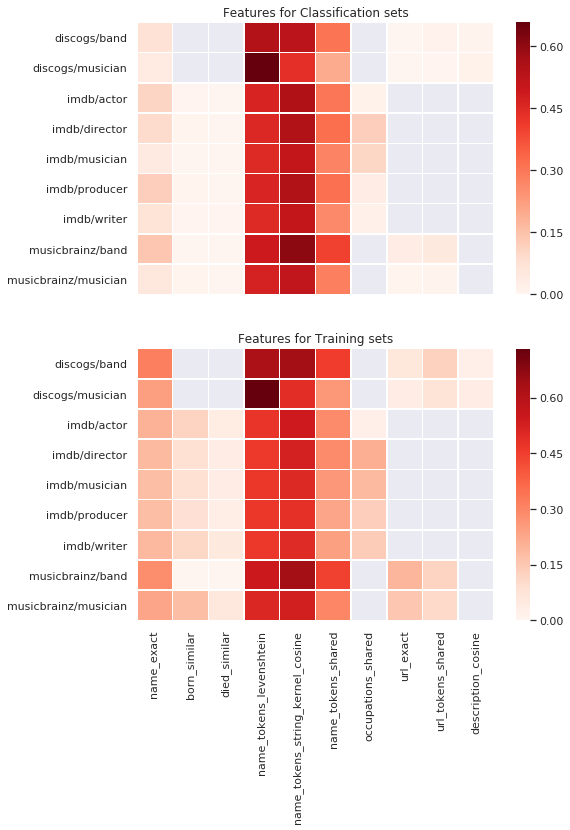
\includegraphics[width=.8\textwidth]{feature_heatmap_classification_and_training} 
  \caption{Average values of the features obtained for each concrete entity. Separated by classification and training datasets.}
  \label{fig:average-features-classification-training}
\end{figure}

\begin{figure}[h]
  \centering 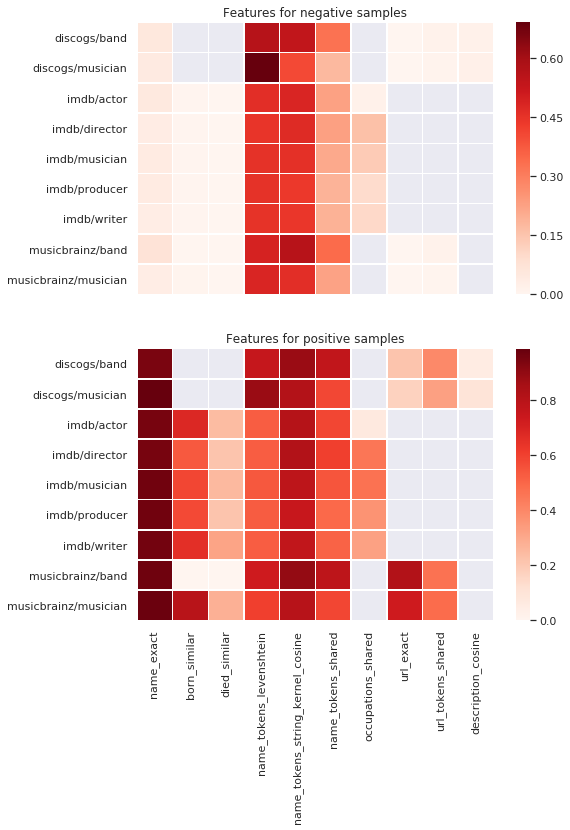
\includegraphics[width=.8\textwidth]{feature_heatmap_training_positive_and_negative} 
  \caption{Average values of the features obtained for each concrete entity. Separated by positive (matches) and negative (non-matches) labelled points in the training data.}
  \label{fig:average-features-positive-negative}
\end{figure}


For completeness, \autoref{sec:apx-feature-distribution} contains distribution plots of the feature values for training and the classification sets, and also for positive and negative samples. 


% PCA of features?
% https://mlens.readthedocs.io/en/0.1.x/getting_started/

% https://www.cs.cmu.edu/~elaw/papers/pca.pdf

%  "On Lines and Planes of Closest Fit to Systems of Points in Space". Philosophical Magazine. 2 (11): 559–572. doi:10.1080/14786440109462720.


\section{Difference between training and real-world data}
\label{sec:training-real-data-difference}

Seeing that the catalogs used are maintained mainly by contributors, one may think that more important people/bands have more information on them than less important ones. From this follows that these entities may have already been linked with the respective external catalog entity. As such, one can assume that the training data is composed mainly of these already labelled \textit{more important} entities, and the classification data are \textit{less important} entities, and less accurately labelled. 

This hypothesis, that training data is better quality than classification data, may impact the ability to extract meaningful features from the data. For example, it may be more common in the classification set than in the training set that an entity has no \textit{birth date}, or that this date is wrong.

\autoref{tab:features-percentage-of-nans-or-zeroes} shows the percentage of zero values obtained for each feature, for each concrete entity. Most features behave similarly across the different sets, for example \textit{nmt.lev} which is always positive. Of more interest are the features \textit{born and die similar}, and \textit{nm.exact}, which are almost always zero in the classification set, but are considerably \textit{better} in the training set.

If training and classification sets were of the same quality then this difference can be attributed to the simple fact that the classification set contains more negative examples than the training set. However, in the current case there is no way to know except by evaluating the classification predictions, which is something that will be automatically done by the Wikidata community once said predictions are uploaded. Regardless, this is something that must be kept in mind since the final performance of the algorithms on the classification data may actually be different from that on the training data. 



\begin{table}[]
\centering
\begin{tabular}{ll|l|l|l|l|l|l|l|l|l|}
\cline{3-11}
                                                       &          & \multicolumn{2}{l|}{discogs} & \multicolumn{5}{l|}{imdb}                       & \multicolumn{2}{l|}{musicbrainz} \\ \cline{3-11} 
                                                       &          & band        & musician       & actor & director & musician & producer & writer & band          & musician         \\ \hline \hline
\multicolumn{1}{|l|}{\multirow{10}{*}{C}} & brn.sim  &             &                & 0.995 & 0.994    & 0.997    & 0.995    & 0.995  & 1.000         & 0.993            \\ \cline{2-11} 
\multicolumn{1}{|l|}{}                                 & des.cos  & 0.919       & 0.850          &       &          &          &          &        &               &                  \\ \cline{2-11} 
\multicolumn{1}{|l|}{}                                 & die.sim  &             &                & 0.999 & 0.999    & 0.999    & 0.998    & 0.997  & 1.000         & 0.998            \\ \cline{2-11} 
\multicolumn{1}{|l|}{}                                 & nm.exct  & 0.923       & 0.960          & 0.893 & 0.909    & 0.958    & 0.878    & 0.930  & 0.860         & 0.949            \\ \cline{2-11} 
\multicolumn{1}{|l|}{}                                 & nmt.lev  & 0.000       & 0.000          & 0.000 & 0.000    & 0.000    & 0.000    & 0.000  & 0.000         & 0.000            \\ \cline{2-11} 
\multicolumn{1}{|l|}{}                                 & nmt.shr  & 0.000       & 0.001          & 0.002 & 0.002    & 0.001    & 0.002    & 0.001  & 0.000         & 0.001            \\ \cline{2-11} 
\multicolumn{1}{|l|}{}                                 & nmt.cos  & 0.064       & 0.058          & 0.000 & 0.000    & 0.000    & 0.000    & 0.000  & 0.005         & 0.001            \\ \cline{2-11} 
\multicolumn{1}{|l|}{}                                 & occ.shr  &             &                & 0.978 & 0.815    & 0.851    & 0.920    & 0.955  &               &                  \\ \cline{2-11} 
\multicolumn{1}{|l|}{}                                 & url.exct & 0.999       & 0.999          &       &          &          &          &        & 0.965         & 0.994            \\ \cline{2-11} 
\multicolumn{1}{|l|}{}                                 & url.shr  & 0.975       & 0.988          &       &          &          &          &        & 0.931         & 0.984            \\ \hline \hline
\multicolumn{1}{|l|}{\multirow{10}{*}{T}}       & brn.sim  &             &                & 0.879 & 0.910    & 0.911    & 0.912    & 0.888  & 1.000         & 0.822            \\ \cline{2-11} 
\multicolumn{1}{|l|}{}                                 & des.cos  & 0.783       & 0.666          &       &          &          &          &        &               &                  \\ \cline{2-11} 
\multicolumn{1}{|l|}{}                                 & die.sim  &             &                & 0.957 & 0.964    & 0.962    & 0.968    & 0.947  & 1.000         & 0.939            \\ \cline{2-11} 
\multicolumn{1}{|l|}{}                                 & nm.exct  & 0.684       & 0.753          & 0.795 & 0.817    & 0.823    & 0.823    & 0.814  & 0.715         & 0.766            \\ \cline{2-11} 
\multicolumn{1}{|l|}{}                                 & nmt.lev  & 0.000       & 0.000          & 0.000 & 0.000    & 0.000    & 0.000    & 0.000  & 0.000         & 0.000            \\ \cline{2-11} 
\multicolumn{1}{|l|}{}                                 & nmt.shr  & 0.000       & 0.000          & 0.001 & 0.001    & 0.001    & 0.000    & 0.000  & 0.000         & 0.001            \\ \cline{2-11} 
\multicolumn{1}{|l|}{}                                 & nmt.cos  & 0.053       & 0.065          & 0.000 & 0.000    & 0.000    & 0.000    & 0.000  & 0.006         & 0.002            \\ \cline{2-11} 
\multicolumn{1}{|l|}{}                                 & occ.shr  &             &                & 0.944 & 0.618    & 0.699    & 0.698    & 0.681  &               &                  \\ \cline{2-11} 
\multicolumn{1}{|l|}{}                                 & url.exct & 0.935       & 0.962          &       &          &          &          &        & 0.805         & 0.843            \\ \cline{2-11} 
\multicolumn{1}{|l|}{}                                 & url.shr  & 0.809       & 0.882          &       &          &          &          &        & 0.750         & 0.806            \\ \hline \hline
\multicolumn{1}{|l|}{\multirow{10}{*}{N}}       & brn.sim  &             &                & 0.995 & 0.996    & 0.996    & 0.997    & 0.995  & 1.000         & 0.992            \\ \cline{2-11} 
\multicolumn{1}{|l|}{}                                 & des.cos  & 0.843       & 0.747          &       &          &          &          &        &               &                  \\ \cline{2-11} 
\multicolumn{1}{|l|}{}                                 & die.sim  &             &                & 0.999 & 0.999    & 0.999    & 0.999    & 0.999  & 1.000         & 0.999            \\ \cline{2-11} 
\multicolumn{1}{|l|}{}                                 & nm.exct  & 0.943       & 0.955          & 0.950 & 0.964    & 0.958    & 0.957    & 0.966  & 0.925         & 0.967            \\ \cline{2-11} 
\multicolumn{1}{|l|}{}                                 & nmt.lev  & 0.000       & 0.000          & 0.000 & 0.000    & 0.000    & 0.000    & 0.000  & 0.000         & 0.000            \\ \cline{2-11} 
\multicolumn{1}{|l|}{}                                 & nmt.shr  & 0.000       & 0.001          & 0.001 & 0.001    & 0.001    & 0.001    & 0.000  & 0.000         & 0.001            \\ \cline{2-11} 
\multicolumn{1}{|l|}{}                                 & nmt.cos  & 0.061       & 0.074          & 0.000 & 0.000    & 0.000    & 0.000    & 0.000  & 0.006         & 0.002            \\ \cline{2-11} 
\multicolumn{1}{|l|}{}                                 & occ.shr  &             &                & 0.965 & 0.685    & 0.765    & 0.764    & 0.746  &               &                  \\ \cline{2-11} 
\multicolumn{1}{|l|}{}                                 & url.exct & 0.999       & 0.998          &       &          &          &          &        & 0.998         & 0.999            \\ \cline{2-11} 
\multicolumn{1}{|l|}{}                                 & url.shr  & 0.959       & 0.967          &       &          &          &          &        & 0.944         & 0.975            \\ \hline \hline
\multicolumn{1}{|l|}{\multirow{10}{*}{P}}       & brn.sim  &             &                & 0.317 & 0.462    & 0.412    & 0.419    & 0.341  & 1.000         & 0.191            \\ \cline{2-11} 
\multicolumn{1}{|l|}{}                                 & des.cos  & 0.637       & 0.370          &       &          &          &          &        &               &                  \\ \cline{2-11} 
\multicolumn{1}{|l|}{}                                 & die.sim  &             &                & 0.756 & 0.782    & 0.747    & 0.783    & 0.682  & 1.000         & 0.718            \\ \cline{2-11} 
\multicolumn{1}{|l|}{}                                 & nm.exct  & 0.055       & 0.013          & 0.047 & 0.045    & 0.034    & 0.036    & 0.037  & 0.032         & 0.023            \\ \cline{2-11} 
\multicolumn{1}{|l|}{}                                 & nmt.lev  & 0.000       & 0.000          & 0.000 & 0.000    & 0.000    & 0.000    & 0.000  & 0.000         & 0.000            \\ \cline{2-11} 
\multicolumn{1}{|l|}{}                                 & nmt.shr  & 0.000       & 0.000          & 0.000 & 0.000    & 0.000    & 0.000    & 0.000  & 0.000         & 0.000            \\ \cline{2-11} 
\multicolumn{1}{|l|}{}                                 & nmt.cos  & 0.035       & 0.031          & 0.000 & 0.000    & 0.000    & 0.000    & 0.000  & 0.009         & 0.002            \\ \cline{2-11} 
\multicolumn{1}{|l|}{}                                 & occ.shr  &             &                & 0.844 & 0.265    & 0.313    & 0.314    & 0.351  &               &                  \\ \cline{2-11} 
\multicolumn{1}{|l|}{}                                 & url.exct & 0.782       & 0.828          &       &          &          &          &        & 0.181         & 0.268            \\ \cline{2-11} 
\multicolumn{1}{|l|}{}                                 & url.shr  & 0.446       & 0.571          &       &          &          &          &        & 0.118         & 0.179            \\ \hline
\end{tabular}
\caption{Percentage of zero values extracted for a given feature, for each concrete entity. Results have been separated by set of procedence: (C)lassification, (T)raining, (N)egative samples, (P)ositive samples.}
\label{tab:features-percentage-of-nans-or-zeroes}
\end{table}



%%%%%%%%%%%%%%%%%%%%%%%%%%%%%%%%%%%%%%%%%

\chapter{Algorithms}
\label{chap:algorithms}

\todo[inline,color=green!25]{Chapter in progress}

This chapter will cover the machine learning algorithms used in the project. The first section will talk about the \textit{baseline} classifiers, a set of standalone classification algorithms. Each algorithm has \textit{hyperparameters}, which are parameters that regulate the functionality of different parts of each algorithm. These are unique to each, and the choice of the best hyperparameter is usually different for diverse problems. \autoref{sec:hyperpar-optimization} will talk about how and according to which procedures the hyperparameters for these baseline algorithms were chosen. Following that, \autoref{sec:ensemble-models} will talk about ensemble models, the motivation for using them, and which techinques for creating them were employed in the project.

As said in \autoref{sec:rl-workflow-linking}, the linking process is one of the main processes in the record linkage workflow. This linking can either be done using a rule-based approach, or a machine learning algorithm can be used to learn when to classify a pair as a match based on the features extracted for that pair. As such, having a well tuned and well performing algorithm is essential for an effective record linkage.

A machine learning algorithm \cite{Russell:2009:AIM:1671238} is an algorithm capable of learning something when given some data. There are many kinds, but those that are of interest for this project are \textit{supervised algorithms}, which are able to draw some inferences about data they've never seen (classification data) when first shown some data similar to that inferences want to be drawn about (training data). 

This capacity of the algorithm of correctly predicting never before seen samples of data is called \textit{generalization}, and it hints at the fact that the algorithm is learning some underlying structure, or patter, in the data it trains on.

For the current project, these algorithms will be shown pairs of entities that are the same, and pairs that are not, and the goal is for the algorithm to discern, for a never seen before pair, whether it is a match or not.


\section{Baseline Classifiers}
\label{sec:baseline-classifiers}

All of the baseline algorithms (except for \textit{mlp} and \textit{slp}, which come from the same family) used are based on a different underlying approach of understanding data and learning something from it. As such, all of these capture the information seen in the training data in different ways. 

The above means that there is a fundamental difference among most of these baseline algorithms, and choosing a \textit{best} one is a very difficult task, since it really depends on the application it is needed for. 

This section strives to explain each baseline algorithm so that the differences among them may be understood. In \autoref{chap:results} the results of these baseline algorithms will be compared against that obtained by the ensemble models (explained in the next section), to see if there is any improvement when employing the idea of considering more than one algorithm to get a prediction. 


\subsection{Linear SVM}
\label{sec:clf-lsvm}

In its simplest sense, SVM \cite{Vapnik1995_svm, Cristianini2000_svm}, and by extension LSVM, are models that learn to segment data into two categories (a binary classifier). The model supposes that the data is sees is spread on a space of $n$ dimensions. When training, the SVM model will learn a hyperplane (which is just an $n-1$-dimensional line) that separates the points in each category by a \textit{gap} which should be wide as possible. The implementation of LSVM used in this project is the one provided by the LIBLINEAR \cite{Fan:2008_liblinear} library, which is accessed using the functionality provided by Scikit-Learn \cite{scikit-learn}. 

Suppose that an SVM gets as training input a series of points in the following format: $(\vec{x}_1, y_1), ..., (\vec{x}_n, y_n)$. Where $\vec{x}_i$ is an  $n$-dimensional vector representing the point, and $y_i$ is the value saying to which class this vector belongs to: either -1 or 1. As said above, the goal is to find a hyperplane which is as far as possible from the nearest points in each group (see \autoref{fig:svm-hyperplan-and-gap}). A hyperplane can be thought of as a series of $\vec{x}$ for which the following is true:

\begin{equation*}
    \vec{w} \cdot \vec{x} - b = 0
\end{equation*}

When classifying new samples, the model will suppose these new samples are points in a space, and then just checks on which side of the hyperplane the new points are, and assign the respective label accordingly. 

SVM algorithm can also modify the input data that they get in such a way that the space representation they learn is different from the one the input data actually represents. This is usually done to map the input data to a higher dimensional space, making it \textit{"easier"} to separate by a gap. This is called the \textit{kernel trick} \cite{Cristianini2000_svm, Boser:1992_kernel_trick}. However, this technique won't be used in the current work since what will be used is an SVM which separates said space \textit{linearly}. The main reason why non-linear SVMs were not used is because the training time for the current implementation offerred by Scikit-Learn is \textquote[][]{... scales at least quadratically with the number of samples and may be impractical beyond tens of thousands of samples}\footurl{https://scikit-learn.org/stable/modules/generated/sklearn.svm.SVC.html\#sklearn.svm.SVC}.

\begin{figure}[H]
  \centering 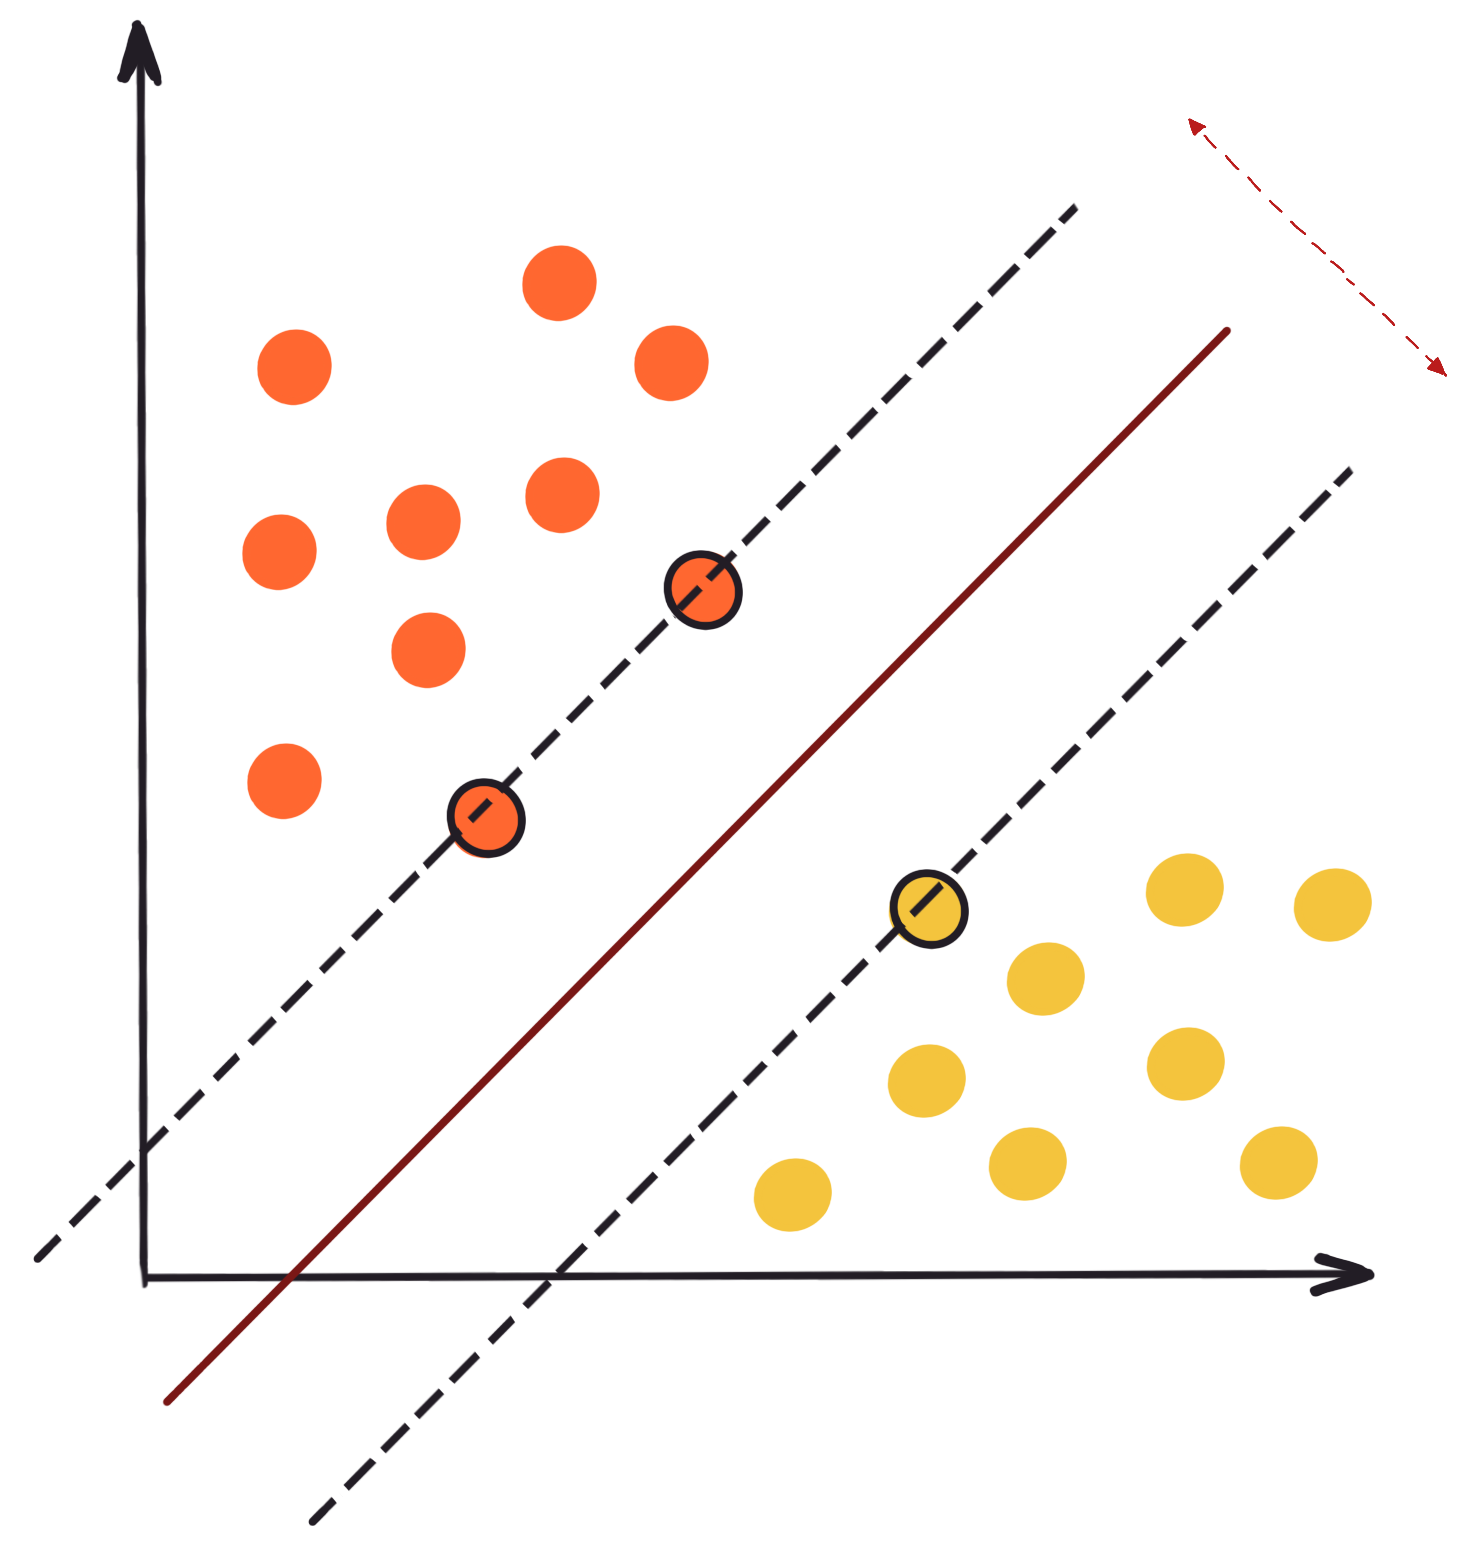
\includegraphics[width=.5\textwidth]{svm_gap_image} 
  \caption{Representation of the hyperplane found by an SVM with the gap that separates the categories. The colored points represent points in the \textit{input space}, each color is a different category. The bold points are the \textit{support vectors} found in this specific instance, which is just another name for points on the margin.}
  \label{fig:svm-hyperplan-and-gap}
\end{figure}

If $\vec{w}$ is the vector defining the hyperplane, then the constraints which define on which side of the margin the data points should be is defined as:

\begin{equation*}
    \begin{cases}
            w^T x_i \geq 1, & \text{if } y_i = 1 \\
            w^T x_i \leq -1, & \text{if } y_i = -1
    \end{cases} 
\end{equation*}

The size of this margin can then be calculated by measuring the distance among the hyperplanes that pass through the points defined at the limits of this constraints (the hyperplanes that go through the support vectors): when they are $w^T x_i = 1$ and $w^T x_i  = -1$ respectively. This distance is given by:

\begin{equation*}
    \frac{2}{\|w\|}
\end{equation*}

And as such, minimizing $\|w\|$, subject to the constraints presented above, will increase the margin while keeping all points correctly classified. 

This is what is called a \textbf{hard margin}, meaning that points must \textit{strictly} be on one side of the margin or the other, and is only useful if the data is linearly separable. The implementation in LIBLINEAR \cite{Fan:2008_liblinear} uses a \textbf{soft margin}, which allows the points to be inside the margin, but adds a penalty which is proportional from the distance to the correct margin. This can be defined by the following optimization problem:

\begin{align*}
    \min_{\|w\|} \frac{1}{2} w^T w + C \sum_{i=1}^n \zeta(w, x_i, y_i) \\ 
    \zeta(w, x_i, y_i) = \max(0, 1-y_i w^T x_i)^2
\end{align*}

Where $w$ is the vector defining the hyperplane, $x_i$ and $y_i$ are the input features and label for element $i$. $C > 0$ is a penalty parameter and $\zeta(w, x_i, y_i)$ is the \textit{penalty function}, which is 0 whenever the $w^T x_i$ gives the correct label. This $w^T x_i$ is $\geq 1$ if $y_i = 1$, and is $\leq -1$ if $y_i = -1$. 

The $C$ parameter regulates how important is it that points are on the correct side of the margin, a higher $C$ will increase the penalty, while a lower $C$ will decrease it. This is a \textit{hyperparameter}, whose choice must be made on a \textit{per problem} basis. 

Note that in many SVM representations there is also a \textit{bias} term $B$ which is part of the equations. In this case, however, the authors of the LIBLINEAR implementation decided to append $B$ to the end of $\vec{w}$ and $\vec{x}$.

The method used to solve this optimization problem is a \textit{coordinate descent method}, presented in \cite{Hsieh:2008_lsvm_coordinated_descent}. Which approximates the optimal $\vec{w}$ by a at most $\epsilon$, which is also called the \textit{tolerance margin}. The approximation is done in $O(log(1/\epsilon))$ iterations. This $\epsilon$ is another hyperparameter that must be tuned for \textit{lsvm}.

Once this optimum $\vec{w}$ is found, then it can be easily used for classification. New points are classified as follows:

\begin{equation*}
    y_p = \begin{cases}
            1, & \text{if } w^Tx > 0 \\
            -1, & \text{otherwise}
          \end{cases} 
\end{equation*}


\subsection{Naive Bayes}
\label{sec:clf-nb}

The implementation used for this classifier is that of \textit{Bernoulli Naive Bayes} \cite{McCallum98acomparison_bayes, Metsis06spamfiltering_bayes} classifier provided by the Scikit-Learn library \cite{scikit-learn}. It expects the features in the input vector $\vec{x}$ to be composed of only \textit{binary values} (\textit{1 or 0}). If the value of a feature is not binary (e.g. 0.6) then it is converted to binary by checking if the value is above a certain threshold \textit{binarize}, if it is then it is converted to 1, and 0 otherwise. This threshold is one of the hyperparameters of this classifier. 

For this model, it is supposed that all features in a feature vector are statistically independent \cite{McCallum98acomparison_bayes} given the class said feature vector represents. 

Suppose that the input to the model is a feature vector $\vec{x}$ where $x_i$ represents the presence of a specific feature $i$ in the vector (either 0 or 1). Suppose also that $y$ stands for one of the possible classes $\vec{x}$ can be assigned to. The probability of getting a class $y$ given the feature vector $\vec{x}$ received as input is:

\begin{equation*}
    P(y | \vec{x} ) = P(y | x_1, x_2, ..., x_n)
\end{equation*}

Using Bayes theorem this can be expressed as:

\begin{equation*}
    P(y | \vec{x}) = \frac{P(y)P(\vec{x} | y)}{P(\vec{x})}
\end{equation*}

Where $P(y)$ is the probability of a given class, and is termed the \textit{prior}. $P(\vec{x} | y)$ is the probability of seeing the specific feature vector considering that vector is of class $y$, this term is named the \textit{likelihood}. Finally, $P(\vec{x})$, which is named the \textit{evidence}, shows how likely is it, in general, to see the given feature vector. 

Since the interest is in finding out which is the actual $y$. Only the \textit{prior} and \textit{likelihood} are necessary for this. The \textit{evidence} can be thought of as a \textit{scaling} constant. By using the \textit{chain rule}, the numerator in the equation above can be presented as the joint probability $P(y)P(\vec{x} | y) = P(x_1, x_2, ..., x_n, y)$. And again by using the chain rule, this can be expressed as:

\begin{equation*}
    P(x_1, x_2, ..., x_n, y) = P(x_1 | x_2, x_3, ..., x_n, y) P(x_2,x_3,...,x_n, y)
\end{equation*}

This process can be continued until the joint probability is expanded to:

\begin{equation*}
    P(x_i | x_{i+1}, x_{i+2}, ..., x_n, y) ... P(x_{n-1}| x_n, y) P(x_n | y) P(y)
\end{equation*}

As said before, the assumption is that all these $x_i$ are independent among themselves given the class $y$ (this is the \textit{naive} assumption in \textit{Naive Bayes}). Because of this, the chain of probabilities above can be shortened to:

\begin{align*}
    P(y)P(\vec{x} | y) & \approx P(x_i | y) P(x_{i+1} | y) ... P(x_n | y) P(y) \\
                           &= P(y) \prod_{i=1}^n P(x_i | y)
\end{align*}

Finally, the original formulation of the probability of a class given the input feature vector can be expressed as

\begin{equation*}
    P(y) | \vec{x}) = \frac{P(y)  \prod_{i=1}^n P(x_i | y)}{P(x_1, x_2, ...,x_n)}
\end{equation*}

The denominator $P(x_1, x_2, ...,x_n)$ is constant given the input, and as such it just scales the probability of the predicted class but holds no actual information about what the class is. To find the class it is only necessary to see which, among the possible classes, has the higher probability. This means that the denominator can be safely ignored.

\begin{equation}
    \hat{y} = \underset{y}{\mathrm{argmax}}\ P(y) \prod_{i=1}^n P(x_i | y)
    \label{eq:naive-bayes}
\end{equation} 

The first term $P(y)$ is simply the frequency of each class: what percentage of the time this class is present in the training data. And the second parameter is defined as follows:

\begin{equation*}
    P(x_i | y) = P(i|y)x_i + (1 - P(i|y))(1-x_i)
\end{equation*}

In the equation above, the first term, $P(i|y)x_i$, is zero when $x_i = 0$, while the second term is zero when $x_i = 1$. The first term indicates the probability of $i$ appearing in class $y$, while the second term is the complement: the probability of not having feature $i$ in class $y$. 

$P(i|y)$ is the smoothed probability of having the feature $i$ appear in the class $y$. This is calculated as follows 

\begin{equation*}
    P(i|y) = \frac{N_{yi} + \alpha}{N_y + \alpha 2}
\end{equation*}

Where $N_{yi} = \sum_{x \in T} x_i$ is the count of all the times feature $i$ appears in class $y$ in the training set $T$. And $N_y = \sum_{i=1}^n N_{yi}$ is the total number of features for $y$ in the training set. $\alpha$ is a hyperparameter of the model and must be set accordingly. However, it is common to set its value $>0$ to account for the problem of getting a feature not seen before. If $\alpha = 0$ and $N_{yi} = 0$ ($i$ has never been seen for $y$ in the training set), then when evaluating \autoref{eq:naive-bayes} the value for $y$ would be 0.

The assumption that the features are independent among themselves means that the probabilities mentioned above can be separately calculated for each feature. This makes naive bayes is efficient even when the input has a high number of dimensions \cite{zhang2004_bayes_optimality}.



\subsection{Logistic Regression}
\label{sec:clf-lr}

Even though it has \textit{regression} in its name, this model is actually a classifier, and is specifically used to make binary predictions. To clarify the meaning of \textit{regression}, it is a machine learning task in which the predicted output is continuous (i.e. a numerical value) instead of a class label. The probability predicted by this classifier is modelled using a logistic function. This function is defined as:
% the goal...
\begin{equation*}
    f(x) = \frac{L}{1 + e^{-k(x-x_0)}}
\end{equation*}

Where $L$ is the maximum value this for function, which for the current application will be 1 since it is a probability. $x_0$ is the value on the $x$-axis at which the function has a value of $L/2$. And $k$ is the steepness of the curve. The function will approaches its limits asymptotically: $L$ as $x$ approaches $+ \infty$, and 0 when it approaches $- \infty$. The following figure shows the curves given by this function with $L=1$, $x_0=0$, and different values for $k$.

\begin{figure}[H]
  \centering 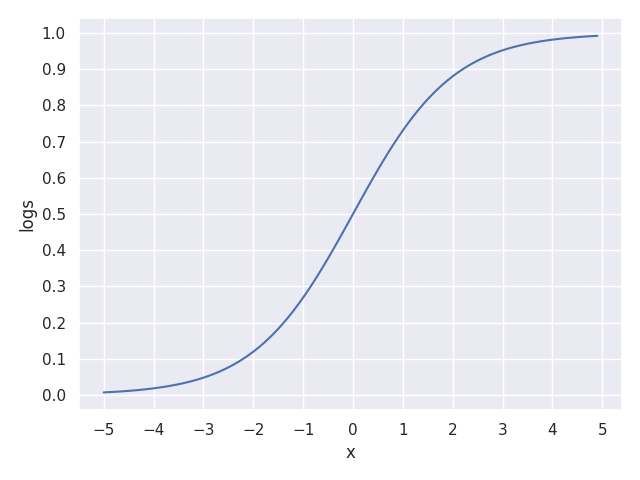
\includegraphics[width=.5\textwidth]{logistic_function} 
\end{figure}

The implementation of logistic regression used for this project works in a similar way as linear SVM, explained in \autoref{sec:clf-lsvm}. In fact, this implementation is also provided by LIBLINEAR \cite{Fan:2008_liblinear}. As \textit{lsvm}, this model proceeds to solve an optimization problem with the data available during training, the formulation is quite similar and the only thing that changes is the \textit{loss function}:

\begin{align*}
    \min_{\|w\|} \frac{1}{2} w^T w + C \sum_{i=1}^n \zeta(w, x_i, y_i) \\ 
    \zeta(w, x_i, y_i) = \log(1+ e^{-y_i w^T x_i})
\end{align*}

This optimization problem is solved with the \textit{coordinate descent method}, presented in \cite{Hsieh:2008_lsvm_coordinated_descent} (which is the same method used to solve the optimization for \textit{lsvm}). Remember that LIBLINEAR appends the bias parameter $B$ to the end of $\vec{w}$ and $\vec{x}$, so this does not appear explicitly in the equation to be optimized. $y_i$ is the class label and should be either -1 or 1. Finally, as for \textit{lsvm}, $C$ is a penalty constant.

The goal is to find the parameters, in this case $\vec{w}$, which best describes best the logistic function that represents the actual probability of an event given the an input vector.  

After training the probability \cite{Fan:2008_liblinear} of a class $y$ given the input vector $\vec{x}$ can be obtained by evaluating the logistic function with the parameters found during optimization.

\begin{equation}
    P(y | \vec{x}) = \frac{1}{1+ e^{-y w^T x}}
\end{equation}on



\subsection{Random Forest}
\label{sec:clf-rgc}

An \textit{ensemble forest} \cite{breiman2001random_forest} is a collection of \textit{decision trees} classifiers. This is actually an ensemble, specifically a \textit{bagging ensemble}, which will be explained in further detain in \autoref{sec:ensemble-models}. The \textit{decision tree} classifier will be explained shortly.

The idea behind \textit{random forest} is to have a collection of \textit{decision trees} which have been trained on different subsets of the data. The idea is to take simple, and potentially unstable models, and join their predictions so that the final predictor has less variace \cite{breiman1996_perturbing}.

When creating a random forest, a collection of $k$ decision trees is created. If the training data $T$ is composed of $n$ samples then each decision tree is trained on $n$ samples. However, instead of giving all trees the same set of samples, what is done is that a new training set $T_i'$ is obtained for each tree. This $T_i'$ is constructed by random sampling, with replacement, until the amount of samples in $T_i'$ is the same as in $T$. \textit{With replacement} means that sampling the same entry from $T$ multiple times is allows. 

Each \textit{decision tree} is trained individually, on their own training set $T_i'$. And when it comes the time to predict the label for a feature vector $x$, the prediction of all decision trees will be asked for, and these will be averaged to get the final prediction \cite{scikit-learn}.

The implementation of \textit{random forest}, and of \textit{decision trees}, comes from the Scikit-Learn \cite{scikit-learn} library.


\subsubsection{Decision Tree}

A \textit{decision tree}, as the name implies, is just a series of simple \textit{decisions rules} which are implied from the data during training. These rules are of form: \textit{if something then do this, otherwise do this other thing}. Most commonly than not, decision trees have multiple levels, meaning that these decisions rules are nested. 

\begin{figure}[H]
  \centering 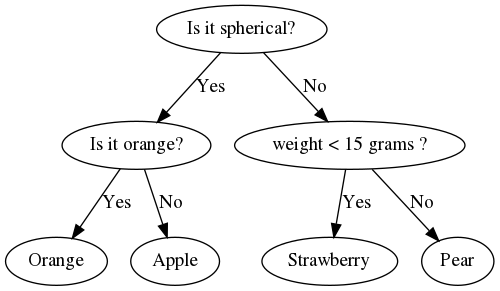
\includegraphics[width=.5\textwidth]{decision_tree} 
  \caption{Example of a decision tree which classify fruits according to their shape, solor, and weight.}
  \label{fig:decision-tree-example}
\end{figure}

It can be seen that at each step in the decision tree in \autoref{fig:decision-tree-example} a test on a different \textit{value} is made, and each branch specifies what to do depending on the outcome of said test. The \textit{leaves} (i.e. the bottom nodes) of the tree specify the outcome of the evaluation. The top node of the tree is called the \textit{root}, and specifies the starting point for the evaluation. 

The first node created for a new decision tree is the \textit{root node}. The way in which the algorithm decides which attribute to test at each node is by finding the test which will make the greatest reduction on the entropy of the subsets, or in other words, the greatest increase in \textit{information gain}. Both of these concepts are explained further in depth below. 

In example \autoref{fig:decision-tree-example} the first test made is on the shape of the fruit, if multiple points are evaluated on this decision tree at the same time then it can thought of as if they splitted at this node: all \textit{spherical} fruits go to the left branch, while all those that are not spherical take the right branch. These two divisions are what are referred two when saying that the entropy is measured on the resulting subsets. 

\textit{Entropy} is no other than the degree of disorder in a set. A completely homogeneous set has an entropy of 0, while the largest value is obtained when the different classes in the set have the same amount of representatives. For the current project, the amount of classes being used is 2 (match and non-match). When using only two classes, the maximum value for the entropy is 1. The total entropy of a set $S$ is measured with the following formula:

\begin{equation*}
    H(S) = \sum_{i=1}^C - p_i \log_2 p_i
\end{equation*}

Where $C$ are all the classes in the set, and $p_i$ is the percentage of times that class $i$ appears in the set. To calculate the entropy of the subsets, after splitting the data on a node, the sum of the entropy of all subsets needs to be calculated. Continuing with the fruits example, say the set coming from the node which did the splitting is $T$, and there are $z \in T$ which are \textit{spherical}, and $k \in T$ which are not. The entropy after splitting on whether the fruit is spherical or not is calculated as: 

\begin{equation*}
    H(S | Spherical) = \frac{|z|}{|T|}H(z) + \frac{|k|}{|T|}H(k)
\end{equation*}

Where $|\cdot|$ denotes the amount of elements in the set. It can be seen that the above is the entropy of each subset weighted by the percentage of elements in that subset with respect to the number of elements in the parent set (which is $T$ in this case). 

In more general terms, the above can be seen as a way in which to measure the total entropy of a set after it has been splitted on an attribute $A$. Finally, the information gain is just the change in entropy obtained when splitting the original set on said $A$.

\begin{equation*}
    IG(S,A) = H(S) - H(S | A)
\end{equation*}

The attribute on which each node splits, for a given dataset, is then selected as:

\begin{equation*}
    \underset{A}{\mathrm{argmax}}\ IG(S, A)
\end{equation*}



\subsection{Single Layer Perceptron}
\label{sec:clf-slp}

The Single Layer Perceptron (SLP) \cite{Goodfellow-et-al-2016} is an algorithm which can learn a linear function by observing some data. Single layer perceptrons have also been used with success in record linkage problems in \cite{Wilson2011_slp_in_rl}. The implementation of SLP used is provided by the Keras library \cite{chollet2015keras}.

For a series on inputs ($\vec{x}, y$), where $\vec{x}$ are vectors of features and $y$ are the classes, an SLP can be thought of a model which learns the following parameters $\vec{w}$ and $b$:

\begin{equation*}
    y_i \approx \lambda(\vec{w} \cdot \vec{x} + b)
\end{equation*}

Where $\vec{w}$ is the vector of weights, which is the same shape as the input vector $\vec{x}$. $\cdot$ is the \textit{dot product} between the input vector and the \textit{weights vector}. $\lambda$ is called the \textit{activation function} and is usually a nonlinear transformation on the weighted sum coming from the inputs. 

The activation function used for this project is the \textit{sigmoid} function, which is very similar to the logistic function defined in \autoref{sec:clf-lr}, and is defined as $\sigma(x) = \frac{1}{1 + e ^ {-x}}$. Using a sigmoid as the activation function allows to interpret the output as the probability of belonging to a class.

The following figure shows an example of a SLP with $\|x\| = \|w\| = 4$.

\begin{figure}[H]
  \centering 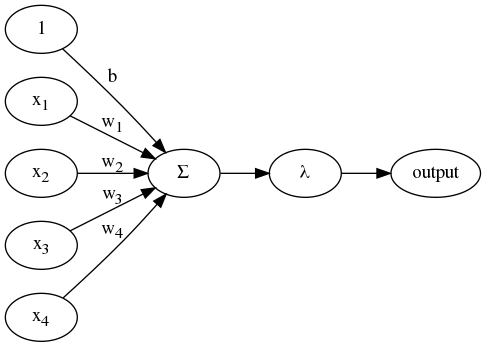
\includegraphics[width=.5\textwidth]{slp_example} 
  \caption{Example of a SLP with 4 inputs.}
  \label{fig:slp-example}
\end{figure}

For completeness, provided below is the algorithm that can be used to learn the parameters $\vec{w}$ and $b$ from samples ($x_i$, $y_i$) in a training set $T$. Note that $y_i'$ is the prediction the perceptron gives for $x_i$. $\delta$ is the learning rate, and is a scalar which regulates how fast the weights are updated. \textit{Epochs} is the amount of times the training set will be processed. For this project, instead of using the basic algorithm mentioned below, the optimization algorithm \textit{Nadam} \cite{dozat2016incorporating_nadam} is used.


\begin{lstlisting}
w, b = initializeWAndB() # initialized to small random values 

for e in 0..(*\textit{epochs}*):
    
    for (*$x_i, y_i$*) in (*$T$*):
        # get prediction
        (*$y_i'$*) = (*$\lambda(\vec{w} \cdot \vec{x} + b)$*)
        (*$dy = y_i - y_i'$*)
        
        # tune the weights based on the error
        (*$w_j = w_j + \delta * dy * x_{i,j}$*)
        
        # update the bias
        (*$b = b + \delta * dy$*)

\end{lstlisting}

SLPs are quite flexible, however it has been shown that they only work well for linearly separable data. In \cite{minsky2017_paupert_xor} it was shown that SLPs cannot learn the XOR function.   




\subsection{Multi-Layer Perceptron}
\label{sec:clf-mlp}


Multi-layer perceptron (MLP \cite{Goodfellow-et-al-2016} is the natural extension of the SLP presented in the last section. As the name implies, with MLP there are multiple perceptrons stacked one after the other. Specifically, an MLP consists of at least three layers: an input layer, one or more hidden layers, and one output layer. Besides having more nodes (which gives MLP more representational power), the main difference between SLP and MLP is that the latter can handle also data which is non-linearly separable.


\begin{figure}[H]
  \centering 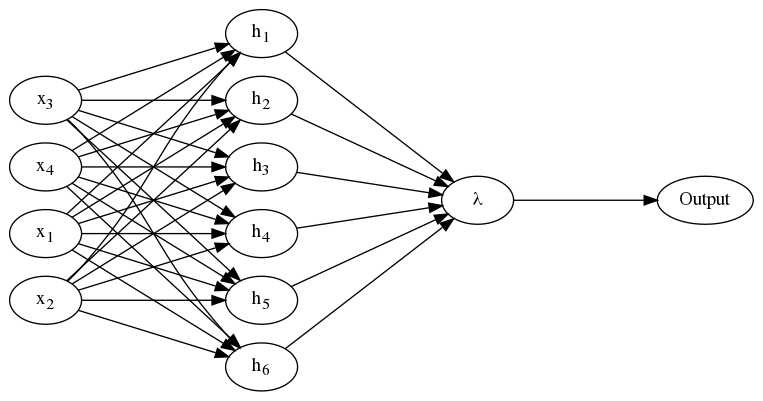
\includegraphics[width=.5\textwidth]{mlp-example} 
  \caption{Example of a MLP with 4 input notes, one hidden layer of size 6, and one output node. Note that to save space the \textit{biases} are not shown in the figure, but each node has one, and it works in the same way as for SLP.}
  \label{fig:mlp-example}
\end{figure}

The example above shows the structure of a MLP. As with SLP, each edge contains a weight the inputs are multiplied by. The inputs and their endpoint nodes in the hidden layer can be thought of as just multiple SLPs (each node in the hidden layer represents one SLP). The output of this SLPs are then used by the following layer as input to that layer's set of perceptrons (also called neurons). Each neuron has its own activation function: for the current work the \textit{sigmoid} function is used as the activation of the output nodes, all other nodes in the hidden layers use \textit{SELU}  \cite{klambauer2017selfnormalizing} which is just a function ensures that negative values grow \textit{slower} than positive values. 


% might be out of scope explaining what SELu is
% \textit{SELU} stands for \textit{scaled exponential linear unit}. It is a function which accepts one parameter and is defined as follows:

Given enough training samples ($\vec{x_i}$, $y_i$), where $\vec{x_i}$ is a feature vector received as input and $y_i$ is the label for said feature vector, a MLP can learn the parameters $\theta$ for a function $f$ such that $y_i \approx f(\vec{x_i}; \theta)$. This parameter $\theta$ is optimized so that the value of the function is as close as possible to the target $y_i$. It has been shown \cite{csaji2001approximation} that, in theory, a MLP with as few as one hidden layer \cite{Hornik1991_approximation}, is able to represent any real function $f*$.

If the weights of a node can be thought of as a vector $\vec{w}$ then the weights of a whole layer can be thought of as a matrix $W$, and the biases for each layer can be represented as a vector $\vec{b}$. With this in mind, the evaluation of the MLP can be done by simply start evaluating from the input and continue until the output. For example, the network presented in the figure above would be evaluated is as follows.

\begin{equation*}
    Output = \lambda_{o}(\vec{b}_{h \to o} + W_{h \to o}^T \cdot \lambda_{h}(\vec{b}_{i \to h} W_{i \to h}^T \cdot \vec{x})) 
\end{equation*}

Where $\vec{x}$ is the input vector. $W_{i \to h}$ and $\vec{b}_{i \to h}$ are the matrix of weights and the bias (respectively) that connect the input layer with the hidden layer. $\lambda_{h}$ is the activation function performed for the hidden layer. $W_{h \to o}$ and  $\vec{b}_{h \to o}$ are the matrix and bias of weights which connect the hidden layer with the output layer. Finally $\lambda_{o}$ is the activation function performed at the output layer.

The above is what is called the \textit{forward pass} when evaluating a MLP. If the parameters $\theta$ still need to be trained then also a backward pass needs to be performed, this ensures that the parameters are updated to learn a specific function.

$\theta$ is nothing more than the collection of weights and biases that the network uses when evaluating a certain input. They are automatically tuned by means of an algorithm called backpropagation \cite{Rumelhart1986}, whose main contribution is that it allows to attribute the classification error to weights which are not directly connected with the output node. This is done by finding the error attributed to each node of the last layer of hidden networks. Then these errors are \textit{propagated back} though each subsequent layer until they reach the input layer. Once the errors for each node are known, the nodes can update their weights by means of \textit{gradient descent}, with just means the weights will be \textit{increased} or \textit{decreased} by a small amount in the direction which decreases the error.

In the current project the used structure of MLP has 4 layers: an input layer, a first hidden layer of 128 neurons, a second hidden layer of 32 neurons, and finally the output layer, with just one output node. Instead of performing the process mentioned above to find the optimal $\theta$ manually, the optimizer \textit{Adadelta} \cite{zeiler2012adadelta} is used. The implementation of MLP used in this project is provided by the Keras library \cite{chollet2015keras}.


\section{Ensemble Models}
\label{sec:ensemble-models}

All of the baseline classifiers presented in the previous section are able to capture specific facets of the data. For example, some may perform better for certain distribution of features and some for others. When using only models from the set of \textit{baseline models} presented above, one by definition needs to choose one of the algorithms and ignores the predictions of the others. Besides this, the task of deciding which parameter is the \textit{best} can be quite difficult, since no model may perform better in all cases. 

Luckily there is the possibility to use more than one model at once, and join the predictions of these \textit{base classifiers} in some way. This is called an \textit{ensemble classifier} \cite{zhou2012ensemble}. There are multiple kinds of ensemble classifiers \cite{opitz1999popular,dietterich2000ensemble}, with the difference being mainly on how they're constructed and how the predictions of the base classifiers are joined. However, in this work only \textit{bagging} and \textit{stacked} ensembles will be explored.

\autoref{sec:motivation-ensemble} will explain the motivation for using an ensemble of models. Following that, \autoref{sec:voting-ensembles} and \autoref{sec:stacked-ensembles} will explain the voting and stacked ensembles used in the project.


\subsection{Motivation} 
\label{sec:motivation-ensemble}

As said in the introduction to this section, different base models may capture different aspects of particular problem. This means that some models may work better than others in some situations. Using an ensemble allows us to mix all of the base model's predictions so that the final classification is as good as possible. It has been shown that joining the predictions of multiple classifiers trained to solve the same problem usually improves the result \cite{opitz1999popular,Hansen1990,Schapire1990}.

Another way this can be seen is that the base classifiers may have a high bias, or high variance, and joining them (e.g. averaging the results) reduces said bias/variance \cite{Breiman1996_bagging_predictors}. As a side note, it is desirable for a machine learning algorithm to have a both low \textit{variance} and a low \textit{bias} \cite{Munro2011_bias_variance_decomp}. However, obtaining both of these is very difficult. A model with high variance \textit{variance} typically overfits the noise in the data, and a model with a high bias tends to underfit the data. 

From the above also follows that a good ensemble is one where the base classifiers are as diverse as possible \cite{zhou2012ensemble}. 

Ensemble models are commonly seen in the top places of machine learning competitions \cite{Bell:2007_netflix_competition}. They have also been successfully employed in diverse areas \cite{zhou2012ensemble} like computer vision, computer security, intrusion detection, in medical applications, among others.

\subsection{Voting Based Ensembles}
\label{sec:voting-ensembles}

Voting based ensembles are a kind of \textit{bagging} ensembles \cite{zhou2012ensemble,Breiman1996_bagging_predictors}. The name of bagging is short for \textit{bootstrapping} and \textit{aggregating}.

% interesting notions https://towardsdatascience.com/ensemble-methods-bagging-boosting-and-stacking-c9214a10a205



% this is implemented by the sklearn library

\subsubsection{Hard Voting Classifier}
\label{sec:hard-voting-classifier}

\subsubsection{Soft Voting Classifier}
\label{sec:soft-voting-classifier}

\subsection{Stack Based Ensembles}
\label{sec:stacked-ensembles}

\subsubsection{Stacked Classifier}
\label{sec:stack-classifier}

% http://citeseerx.ist.psu.edu/viewdoc/summary?doi=10.1.1.56.1533
% http://statistics.berkeley.edu/sites/default/files/tech-reports/367.pdf
% Doc diss on super learnear https://www.stat.berkeley.edu/~ledell/papers/ledell-phd-thesis.pdf

% this is implemented by the mlens library


\subsubsection{Gated Classifier}
\label{sec:gated-classifier}

Gated ensembles can be thought of as a mix between a stacked and a bagging ensembles. As in the bagging ensemble, the \textit{gated} ones also have a single pool of classifier whose predictions are joined to together. However, unlike with bagging, the gated ensemble uses a meta layer to weight this predictions (as does the stacked ensemble).

Recall that with bagging there are two options to mix the \textit{opinions} of the base classifiers: either their predictions get averaged and the highest of this is chosen as the final prediction, or a \textit{majority vote} is held and the class with more votes is the final chosen one. The approach taken with gated ensembles is very similar to the \textit{averaging} case presented above. However, before averaging, the predictions of the base classifiers are weighted, so the final operation is just a weighted average.

However, manually finding these weights can be quite hard. That is why it is best to delegate this task to another machine learning algorithm. In principle any learning algorithm can be used to as this final meta layer (which is the same term also used for the final layer of stacked ensembles). 

% Note that both stacked and gated are instances of superlearner, which is a stacking algorithm

% this is implemented by the mlens library



\chapter{Results}
\label{chap:results}

This chapter presents the results obtained when evaluating the different models, both baseline and ensembles. The evaluation results for both the baseline and ensemble classifiers presented in this section have been obtained by performing a 5-fold cross validation procedure on the training data (on overview of which is given in the next section). The data used to generate this results was the Wikidata training dumps and the external catalog dumps mentioned in \autoref{sec:orig-shape-of-data}.

Before training and evaluating the baseline models, a grid search was performed to find the best hyperparameters for each of these. This is explained in \autoref{sec:hyperpar-optimization}.

The metrics measured during evaluation are: \textit{F1 score}, \textit{Precision}, and \textit{Recall}. These have been previously explained in \autoref{sec:rl-workflow-evaluation}. 

Note that this section includes only the results obtained during evaluation. In the appendix, specifically in \autoref{sec:apx-classification-results} a brief analysis of the distribution of predictions obtained when predicting on the classification set can be found.

Besides presenting the results, \autoref{sec:sec:comparative-evaluation} will strive to compare the results obtained for the baseline and ensemble models, and point out any differences.


\section{Cross Validation}
\label{sec:cross-validation}

When evaluating the performance of a given machine learning algorithm, it is desirable to know what the performance of said algorithm will be on the real world data\footnote{also known as \textit{classification} data, or classification set} the one for which the final values want to be known. However, it is impossible to do so, because this would require to have a labelled version of this real world data. 

Ideally, the training data should come from a distribution similar to the classification data, if not the performance of the algorithm will not be satisfactory when applied to the classification set. This assumption, that the training and classification datasets are \textbf{i.i.d.}\footnote{Independent and identically distributed.} \cite{clauset2011brief}, allows us to take a piece of the training set and set it aside to act as an \textit{approximation} of the classification set. This piece we set aside is called the \textit{test set}. 

The way this can be used is that we separate the whole training data $D$ into a \textit{test set} $S$ and a \textit{training set} $T$ such that:

\begin{align*}
    S &\cup T = D \\ 
    S &\cap T = \varnothing
\end{align*}

The learning algorithm is then trained only on $T$, and finally an estimate of the error the algorithm will get when predicting the real classification data can be obtained by measuring the error obtained when predicting $V$. 

It is important that the conditions mentioned above are respected for this to work. Especially $S \cap T = \varnothing$, since if any element $S_i \in T$ then the algorithm will have seen the actual label of said element during training, and this may influence the estimate performance calculated on the test set since the classification set is unknown to the algorithm at prediction time. The algorithm may have learned the label for said item, and as such will affect the final error measure on the validation set by making it look better than it actually is.

Another consideration to keep in mind is that the actual validation set should not be used to tune the hyperparameters of the algorithm, since this will only make the algorithm perform better in the validation data, but not necessarily better in the classification data. Once again, this may cause the performance of the algorithm to seem better than it actually is. To tune hyperparameters what can be done is separating the training data into a further third set, called the \textit{validation set} $V$, which is also subject to $V \cap T \cap S = \varnothing$. With this, now the training can be done on $T$, hyperparameters can be tuned to minimize the error on $V$, and finally the estimate of the classification set error can be obtained by evaluating the algorithm on $S$.

In some cases, however, this is not desirable since it means the training data will be split three ways, and a big part of it will not be actually seen by the model at all. An example case may be when there is only a small training set, or the algorithm being used needs a lot of data to be trained properly (e.g. when using a neural network).

Another possible problem may be that the error metrics obtained may be dependent on the specific separation of the dataset that was made to create $T$, $V$, and $S$. For example, the algorithm may appear to have a great performance on $S$, but if the training set were to be shuffled and split again then the performance would be much worse.

A better approach, which permits the use of most of the training data, and also provide an approximation of a \textit{split-independent} error value is to use k-fold cross validation \cite{Kohavi:1995_study_of_cross_validation,Cawley:2010_crossval_model_selection}. In this process, we repeatedly ($k$ times) split the training set $D$ into $T$ and $V$ as mentioned above, train on the current split $T$, measure the error on $V$ and then average all the error measures to get a final error. Using a $k > 1$ reduces variability in the final error metric since these get averaged over many possible ways of splitting the training data.

The algorithm for $k$-fold cross validation is as follows:

\begin{lstlisting}
errors = [] # list that will hold the errors obtained during each fold
for i in 0..(*$k$*):
    (*$T, V$*) (*$\leftarrow$*) splitTrainingData((*$D$*))
    
    (*$V_{features}, V_{labels}$*) (*$\leftarrow$*) getFeaturesAndLabels((*$V$*))
    (*$T_{features}, T_{labels}$*) (*$\leftarrow$*) getFeaturesAndLabels((*$T$*))

    model = initializeClassifier()
    model.fit((*$T_{features}, T_{labels}$*)) # train the classifier
    
    predictions = model.predict((*$V_{features}$*))
    
    error = measureError(predictions, (*$V_{labels}$*))
    errors.append(error)
    
finalError = average(errors)
\end{lstlisting}

Note that in this example \textit{error} was mentioned as the metric that is being extracted. However, any metric which depends on $V$ can be extracted in such a way. For this work, the metrics obtained during the cross validation procedure are \textit{F1-Score}, \textit{Precision}, and \textit{Recall}.


\section{Baseline Hyperparameter Optimization}
\label{sec:hyperpar-optimization}

As seen in \autoref{chap:algorithms}, all classifiers have hyperparameters which can be tuned to change the behaviour of each algorithm. Setting the correct value for these hyperparameters is essential to get a good performance from them. 

Finding the best hyperparameter for a model usually involves a lot of manual tinkering, trying different combinations until the best set of hyperparameters is found. This procedure can actually be automated by using the \textit{Grid Search} \cite{claesen2015hyperparameter} functionality provided by Scikit-Learn \cite{scikit-learn}. In grid search, a set of possible values for each hyperparameter is provided, and the algorithm will go through each possible combination of these and tries them on the classifier. 

The classifier is evaluated using each combination of hyperparameters, and finally the combination which provided the best evaluation performance is returned. This is a lengthy process but since the evaluations are independent of each other they can be done in parallel \cite{Bergstra:2012_random_gs}.

For the current project, the evaluation of the hyperparameters was done by performing a 5-fold cross validation with the classifier initialized using the specified parameters. After the 5-fold cross validation is complete, the average performance of these is returned. The \textit{grid search} eventually returns the combination of hyperparameters which gave the best \textit{average} performance while executing the \textit{cross validation}.

Since the grid search procedure, plus the 5-fold cross validation, is quite a lengthy procedure, it was chosen to perform this optimization by only evaluating the performance of the models on \textit{Discogs/Musician}. The procedure searches for the combination of hyperparameters which makes the classifier give the best \textit{F1} score.

The following tables show the hyperparameters tried for each for each baseline algorithm. In bold are the hyperparameter which were chosen as the best by the grid search procedure. 

\todo[inline,color=blue!25]{explain those parameters that weren't mentioned in the model description.}

\subsubsection{Naive Bayes}

\begin{table}[H]
\centering
\begin{tabular}{l|l}
alpha           & binarize     \\ \hline
1               & 0.9          \\
0.1             & 0.8          \\
0.01            & 0.7          \\
0.001           & 0.6          \\
\textbf{0.0001} & 0.5          \\
                & 0.4          \\
                & 0.3          \\
                & \textbf{0.2} \\
                & 0.1     
\end{tabular}
\end{table}


\subsubsection{Logistic Regression}

\begin{table}[H]
\centering
\begin{tabular}{l|l|l|l|l}
C            & class\_weight & max\_iter    & solver             & tol            \\ \hline
100          & balanced      & 200          & sag                & 1e-05          \\
10           & \textbf{None} & \textbf{100} & saga               & 0.0001         \\
\textbf{1.0} &               &              & lbfgs              & \textbf{0.001} \\
0.1          &               &              & \textbf{liblinear} &                \\
0.01         &               &              &                    & 
\end{tabular}
\end{table}


\subsubsection{Linear SVM}

\begin{table}[H]
\centering
\begin{tabular}{l|l|l|l}
C            & dual          & max\_iter     & tol            \\ \hline
100          & False         & 2000          & 1e-05          \\
10           & \textbf{True} & \textbf{1000} & 0.0001         \\
\textbf{1.0} &               &               & \textbf{0.001} \\
0.1          &               &               &                \\
0.01         &               &               & 
\end{tabular}
\end{table}


\subsubsection{Random Forest}

\begin{table}[H]
\centering
\begin{tabular}{l|l|l|l}
bootstrap     & criterion        & max\_features & n\_estimators \\ \hline
False         & \textbf{entropy} & \textbf{None} & \textbf{500}  \\
\textbf{True} & gini             & log2          & 350           \\
              &                  & sqrt          & 200           \\
              &                  &               & 100          
\end{tabular}
\end{table}


\subsubsection{Single Layer Perceptron}

\begin{table}[H]
\centering
\begin{tabular}{l|l|l|l}
activation       & batch\_size  & epochs        & optimizer      \\ \hline
\textbf{sigmoid} & 2048         & 3000          & \textbf{Nadam} \\
                 & 1024         & 2000          & Adadelta       \\
                 & 512          & \textbf{1000} & RMSprop        \\
                 & \textbf{256} & 100           & adam     
\end{tabular}
\end{table}


\subsubsection{Multi-Layer Perceptron}

\begin{table}[H]
\centering
\begin{tabular}{l|l|l|l|l|l}
batch\_size  & epochs        & hidden\_activation & hidden\_layer\_dims    & optimizer         & output\_activation \\ \hline
\textbf{512} & 2000          & \textbf{selu}      & {[}128, 32, 32{]}      & Nadam             & \textbf{sigmoid}   \\
             & \textbf{1000} & tanh               & {[}256, 128, 32{]}     & \textbf{Adadelta} &                    \\
             &               & relu               & \textbf{{[}128, 32{]}} & adam              & 
\end{tabular}
\end{table}



\section{Baseline Evaluation}
\label{sec:baseline-evaluation}

This section presents the results of performing a 5-fold cross validation on the baseline models presented in \autoref{sec:baseline-classifiers}. 

The table below shows the performance metrics for each classifier applied to each concrete entity. Note that the names of the algorithms have been shortened to make the table fit nicely in the page. The abbreviations are as follow:

\begin{itemize}
    \item Linear Support Vector Machine: lsvm
    \item Logistic Regression: lr
    \item Multi layer perceptron: mlp
    \item Naive Bayes: nb
    \item Random Forest: rf
    \item Single layer perceptron: slp
\end{itemize}


\begin{longtable}{|l|l|l|l|l|l|l|l|l|}
\hline
Catalog     & Entity   & Model & F1.Mean  & F1.STD   & Prec.Mean & Prec.STD & Rec.Mean & Rec.STD  \\ \hline
discogs     & musician & lsvm  & 0.936944 & 0.001224 & 0.905424  & 0.002080 & 0.970741 & 0.000880 \\
discogs     & band     & lsvm  & 0.925262 & 0.001267 & 0.896373  & 0.002110 & 0.956090 & 0.003388 \\
imdb        & actor    & lsvm  & 0.894011 & 0.000789 & 0.875260  & 0.002088 & 0.913592 & 0.001998 \\
imdb        & director & lsvm  & 0.912727 & 0.001597 & 0.880551  & 0.005850 & 0.947397 & 0.003670 \\
imdb        & musician & lsvm  & 0.917906 & 0.001399 & 0.909440  & 0.002345 & 0.926534 & 0.001067 \\
imdb        & producer & lsvm  & 0.905975 & 0.003885 & 0.894173  & 0.006799 & 0.918114 & 0.001219 \\
imdb        & writer   & lsvm  & 0.928606 & 0.001983 & 0.919005  & 0.002274 & 0.938421 & 0.003574 \\
musicbrainz & musician & lsvm  & 0.954410 & 0.001406 & 0.942882  & 0.002112 & 0.966225 & 0.001090 \\ 
musicbrainz & band     & lsvm  & 0.913877 & 0.001689 & 0.961199  & 0.003976 & 0.871046 & 0.006050 \\ \hline
discogs     & musician & lr    & 0.938138 & 0.001693 & 0.917022  & 0.002191 & 0.960250 & 0.001370 \\
discogs     & band     & lr    & 0.924791 & 0.001550 & 0.908952  & 0.001476 & 0.941198 & 0.003025 \\
imdb        & actor    & lr    & 0.893573 & 0.000579 & 0.878388  & 0.001838 & 0.909299 & 0.001406 \\
imdb        & director & lr    & 0.913846 & 0.000694 & 0.892154  & 0.004468 & 0.936658 & 0.003834 \\
imdb        & producer & lr    & 0.906045 & 0.002643 & 0.898064  & 0.005640 & 0.914192 & 0.000826 \\
imdb        & musician & lr    & 0.917958 & 0.001717 & 0.908442  & 0.002911 & 0.927680 & 0.001280 \\
imdb        & writer   & lr    & 0.928108 & 0.002082 & 0.924621  & 0.001792 & 0.931635 & 0.004264 \\
musicbrainz & musician & lr    & 0.953083 & 0.001301 & 0.943755  & 0.002042 & 0.962600 & 0.001165 \\ 
musicbrainz & band     & lr    & 0.918022 & 0.002327 & 0.937643  & 0.002251 & 0.899217 & 0.003973 \\ \hline
discogs     & musician & mlp   & 0.940715 & 0.001443 & 0.921507  & 0.001770 & 0.960754 & 0.003867 \\
discogs     & band     & mlp   & 0.928931 & 0.001310 & 0.915249  & 0.001875 & 0.943032 & 0.001727 \\
imdb        & actor    & mlp   & 0.896922 & 0.000400 & 0.880657  & 0.003412 & 0.913832 & 0.004129 \\
imdb        & director & mlp   & 0.919340 & 0.000980 & 0.899994  & 0.002724 & 0.939548 & 0.002002 \\
imdb        & musician & mlp   & 0.925888 & 0.001165 & 0.942860  & 0.001545 & 0.909520 & 0.001863 \\
imdb        & producer & mlp   & 0.909398 & 0.002913 & 0.894253  & 0.007249 & 0.925119 & 0.003188 \\
imdb        & writer   & mlp   & 0.930302 & 0.002571 & 0.924571  & 0.003714 & 0.936149 & 0.006365 \\
musicbrainz & musician & mlp   & 0.957375 & 0.001629 & 0.944146  & 0.004491 & 0.971004 & 0.002647 \\ 
musicbrainz & band     & mlp   & 0.921134 & 0.002588 & 0.926546  & 0.004402 & 0.915818 & 0.004989 \\ \hline
discogs     & musician & nb    & 0.931622 & 0.001314 & 0.903489  & 0.002155 & 0.961565 & 0.000812 \\
discogs     & band     & nb    & 0.922386 & 0.001457 & 0.891462  & 0.001633 & 0.955542 & 0.003274 \\
imdb        & actor    & nb    & 0.889563 & 0.001311 & 0.825956  & 0.002002 & 0.963789 & 0.001153 \\
imdb        & musician & nb    & 0.904327 & 0.013959 & 0.868388  & 0.055110 & 0.948158 & 0.033475 \\
imdb        & producer & nb    & 0.898657 & 0.004254 & 0.842785  & 0.008230 & 0.962525 & 0.001450 \\
imdb        & director & nb    & 0.907755 & 0.002541 & 0.855312  & 0.005063 & 0.967075 & 0.001997 \\
imdb        & writer   & nb    & 0.922121 & 0.002580 & 0.882778  & 0.004051 & 0.965145 & 0.002172 \\
musicbrainz & musician & nb    & 0.952783 & 0.001847 & 0.953561  & 0.002394 & 0.952008 & 0.001847 \\
musicbrainz & band     & nb    & 0.907094 & 0.001994 & 0.953012  & 0.001335 & 0.865401 & 0.002974 \\ \hline
discogs     & musician & rf    & 0.933460 & 0.002427 & 0.917496  & 0.003021 & 0.949992 & 0.002296 \\
discogs     & band     & rf    & 0.921673 & 0.001084 & 0.909216  & 0.002648 & 0.934490 & 0.002988 \\
imdb        & actor    & rf    & 0.899161 & 0.000836 & 0.879621  & 0.001427 & 0.919592 & 0.001620 \\
imdb        & director & rf    & 0.916903 & 0.000940 & 0.892806  & 0.003096 & 0.942355 & 0.002601 \\
imdb        & musician & rf    & 0.922135 & 0.000594 & 0.932216  & 0.000733 & 0.912272 & 0.001018 \\
imdb        & producer & rf    & 0.906239 & 0.004720 & 0.895270  & 0.008984 & 0.917553 & 0.005214 \\
imdb        & writer   & rf    & 0.929301 & 0.002919 & 0.922216  & 0.004160 & 0.936508 & 0.003393 \\
musicbrainz & musician & rf    & 0.953673 & 0.001146 & 0.943972  & 0.001591 & 0.963577 & 0.001052 \\ 
musicbrainz & band     & rf    & 0.918844 & 0.002231 & 0.938321  & 0.005419 & 0.900192 & 0.003714 \\ \hline
discogs     & musician & slp   & 0.938168 & 0.001664 & 0.917755  & 0.002291 & 0.959510 & 0.001258 \\
discogs     & band     & slp   & 0.925647 & 0.001462 & 0.908264  & 0.001465 & 0.943716 & 0.003188 \\
imdb        & actor    & slp   & 0.893205 & 0.000591 & 0.881499  & 0.001829 & 0.905232 & 0.001676 \\
imdb        & director & slp   & 0.914070 & 0.000545 & 0.895414  & 0.003822 & 0.933551 & 0.003516 \\
imdb        & musician & slp   & 0.917503 & 0.001383 & 0.909845  & 0.002659 & 0.925296 & 0.000865 \\
imdb        & producer & slp   & 0.905526 & 0.002380 & 0.903146  & 0.006456 & 0.907958 & 0.001993 \\
imdb        & writer   & slp   & 0.927724 & 0.001915 & 0.924983  & 0.002891 & 0.930499 & 0.003970 \\
musicbrainz & musician & slp   & 0.953054 & 0.001383 & 0.943662  & 0.002094 & 0.962638 & 0.001341 \\
musicbrainz & band     & slp   & 0.915977 & 0.002302 & 0.946439  & 0.002538 & 0.887441 & 0.005184 \\ \hline
\end{longtable}


The columns name \textit{*.Mean} are the mean value of the relative metric obtained during the cross validation procedure. Similarly, the columns named \textit{*.STD} are the standard deviation of said metrics. 

It's interesting to note that the best \textit{F1.Mean} for all models seems to have been obtained on the entity \textit{Musicbrainz/Musician}, and the second best for \textit{Discogs/Musician}. For most of the models, the third best \textit{F1.Mean} is obtained on \textit{IMDb/Writer} (only Naive Bayes has \textit{Discogs/Band} as the third best, although the values are very similar with \textit{Writer}).

When it comes to \textit{precision} things are less \textit{unanimous}. Most models still have \textit{Musicbrainz/Musician} as their best precision, except for \textit{lsvm}, and \textit{slp}, who both have \textit{Musicbrainz/Band}, although for this the second best is also \textit{Musicbrainz/Musician}. The place of second best precision among the first set of classifiers is \textit{Musicbrainz/Band}, except for \textit{mlp}, who has \textit{IMDb/Musician} in the second place. 

For \textit{Recall}, all models except for \textit{lsvm} and \textit{Naive Bayes} have \textit{Musicbrainz/Musician} as their top concrete entity. \textit{lsvm} and \textit{naive bayes} have \textit{Discogs/Musician} and \textit{IMDb/Director} respectively. All models except \textit{lsvm} and \textit{Naive Bayes} have \textit{Discogs/Musician} as their second best. \textit{lsvm} and \textit{naive bayes} have \textit{Musicbrainz/Musician} and \textit{IMDb/Writer} respectively.

The results presented above are quite interesting since they show that features extracted for \textit{Musicbrainz/Musicians} are more informative than those for other concrete entities. Another reason for this may be, as seen in \autoref{sec:feature-viz}, that the \textit{Musicbrainz} catalogs has eight possible features while all other catalogs have seven. 

The table below shows which was the average performance of each model on each catalog in general. The rows have been ordered by \textit{F1 Score}. It can be noted that the average \textit{STD} is quite low compared to the score values. 

\begin{longtable}{|l|l|l|l|l|l|l|l|}
\hline
Catalog     & Model & Avg.F1   & Avg.F1.STD & Avg.Prec & Avg.Prec.STD & Avg.Rec  & Avg.Rec.STD \\ \hline
musicbrainz & mlp   & 0.939254 & 0.002109   & 0.935346 & 0.004446     & 0.943411 & 0.003818    \\
musicbrainz & rf    & 0.936259 & 0.001688   & 0.941146 & 0.003505     & 0.931885 & 0.002383    \\
musicbrainz & lr    & 0.935553 & 0.001814   & 0.940699 & 0.002146     & 0.930909 & 0.002569    \\
musicbrainz & slp   & 0.934516 & 0.001842   & 0.945051 & 0.002316     & 0.925040 & 0.003263    \\
musicbrainz & lsvm  & 0.934144 & 0.001548   & 0.952041 & 0.003044     & 0.918635 & 0.003570    \\
musicbrainz & nb    & 0.929939 & 0.001920   & 0.953287 & 0.001865     & 0.908705 & 0.002410    \\ \hline
imdb        & mlp   & 0.916370 & 0.001606   & 0.908467 & 0.003729     & 0.924834 & 0.003509    \\
imdb        & rf    & 0.914748 & 0.002002   & 0.904426 & 0.003680     & 0.925656 & 0.002769    \\
imdb        & lr    & 0.911906 & 0.001543   & 0.900334 & 0.003330     & 0.923893 & 0.002322    \\
imdb        & lsvm  & 0.911845 & 0.001931   & 0.895686 & 0.003871     & 0.928812 & 0.002306    \\
imdb        & slp   & 0.911606 & 0.001363   & 0.902977 & 0.003531     & 0.920507 & 0.002404    \\
imdb        & nb    & 0.904485 & 0.004929   & 0.855044 & 0.014891     & 0.961338 & 0.008049    \\ \hline
discogs     & mlp   & 0.934823 & 0.001377   & 0.918378 & 0.001822     & 0.951893 & 0.002797    \\
discogs     & slp   & 0.931907 & 0.001563   & 0.913009 & 0.001878     & 0.951613 & 0.002223    \\
discogs     & lr    & 0.931464 & 0.001622   & 0.912987 & 0.001833     & 0.950724 & 0.002197    \\
discogs     & lsvm  & 0.931103 & 0.001246   & 0.900899 & 0.002095     & 0.963415 & 0.002134    \\
discogs     & rf    & 0.927566 & 0.001755   & 0.913356 & 0.002835     & 0.942241 & 0.002642    \\
discogs     & nb    & 0.927004 & 0.001386   & 0.897476 & 0.001894     & 0.958554 & 0.002043    \\ \hline
\end{longtable}



\begin{table}[H]
\centering
\begin{tabular}{l|l|l|l}
                                  & Best Avg.F1 & Best Avg.Prec & Best Avg.Rec \\ \hline
\multicolumn{1}{l|}{Musicbrainz} & mlp    & nb       & mlp     \\ \hline
\multicolumn{1}{l|}{IMDb}        & mlp    & mlp      & nb      \\ \hline
\multicolumn{1}{l|}{Discogs}     & mlp    & mlp      & lsvm    \\ 
\end{tabular}
\caption{Best performing baseline models for each catalog according to the three main metrics.}
\label{tab:best-model-per-metric-average}
\end{table}

It seems that overrall \textit{mlp} is the best performing baseline model. It is interesting to note that although \textit{naive bayes} appears to have the highest \textit{precision} for \textit{Musicbrainz} is is also the model that has the lowest \textit{recall} for that same catalog. The same happens for IMDb, \textit{naive bayes} has the best \textit{recall} but the lowest precision. A slight exception is Discogs, where \textit{lsvm} has the best \textit{recall}, and is the second worst in \textit{precision}.



Finally, the table below contains a summary of the metrics obtained by each classifier, these were obtained by averaging the metrics obtained for each concrete entity. The best value for each metric is denoted in \textbf{bold}.

\begin{table}[H]
\centering
\begin{tabular}{l|l|l|l|l|l|l}
Model & Avg.F1   & Avg.F1.STD & Avg.Prec & Avg.Prec.STD & Avg.Recall & Avg.Recall.STD \\ \hline
mlp   & \textbf{0.925556} & 0.001667   & \textbf{0.916643} & 0.003465     & 0.934975   & 0.003420       \\
rf    & 0.922377 & 0.001877   & 0.914570 & 0.003453     & 0.930726   & 0.002655       \\
lr    & 0.921507 & 0.001621   & 0.912116 & 0.002734     & 0.931414   & 0.002349       \\
slp   & 0.921208 & 0.001514   & 0.914556 & 0.002894     & 0.928427   & 0.002555       \\
lsvm  & 0.921080 & 0.001693   & 0.909367 & 0.003293     & 0.934240   & 0.002548       \\
nb    & 0.915145 & 0.003473   & 0.886305 & 0.009108     & \textbf{0.949023}   & 0.005462          
\end{tabular}
\caption{Average metrics obtained for the baseline classifiers.}
\label{tab:metrics-summary-baseline}
\end{table}


It can be seen in \autoref{tab:metrics-summary-baseline} that \textit{mlp} is the model with the best \textit{F1 score} (as expected). It also seems that \textit{mlp} has the best average \textit{precision} and is second in best \textit{recall}, with the first place being taken by \textit{naive bayes}.

\begin{figure}[H]
  \centering 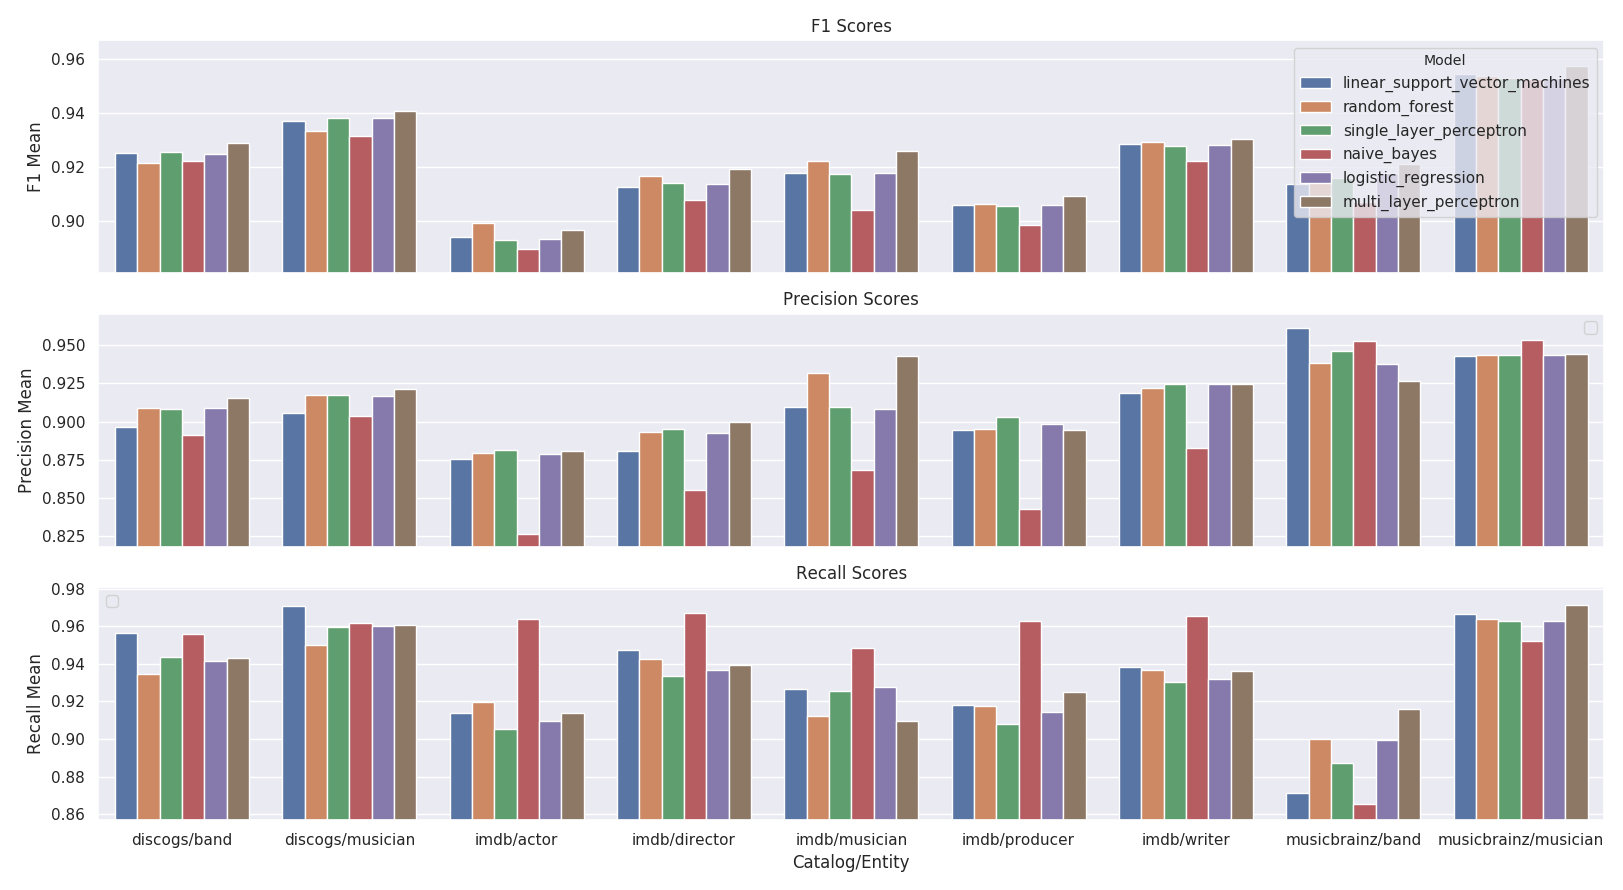
\includegraphics[width=\textwidth]{baseline_evluation_main_metrics_barplot} 
  \caption{Barplots of the evaluation metrics for the baseline models. Separated by concrete entity.}
  \label{fig:baseline-evaluation-barplots}
\end{figure}

A graphical representation of the table above can be seen in \autoref{fig:baseline-evaluation-barplots}. Here it can be better appreciated which concrete entities are easier to classify for which algorithms. For instance, it seems that all models have trouble with \textit{IMDb/Actor}, in all metrics. It can also be seen that \textit{naive bayes} tends to have a high recall in all cases, and poor \textit{precision} in most. Another interesting thing to note is that all models have a much lower recall for \textit{Musicbrainz/Band}, even if the precision they attain for this same entity is quite good when compared against the others. As expected, \textit{Musicbrainz/Musician} is the overall best classified concrete entity. 

It can also be appreciated that while \textit{mlp} almost always has the best performance, some other models may have similar or event better scores for some metrics. For instance, all models have a higher precision for \textit{Musicbrainz/Band} than \textit{mlp}, and most have a higher recall for \textit{IMDb/Musician}. This suggests that using only the \textit{opinion} of \textit{mlp} would not be the optimal strategy to get the best performance. A better approach would be to mix these predictions by means of an ensemble method.



\section{Ensemble Evaluation}
\label{sec:ensemble-evaluation}

This section presents the results obtained during the 5-fold cross validation procedure when applied to the ensemble models presented in \autoref{sec:ensemble-models}. The results are presented once for each concrete entity and model. Note that the names of the ensemble classifiers have been shortened to make the table fit properly. Below is the mapping from the full names of the classifiers to their shortened version/ 

\begin{itemize}
    \item Gated Classifier : gc
    \item Stacked Classifier : sc
    \item Hard Voting Classifier : vh
    \item Soft Voting Classifier : vs
\end{itemize}


\begin{longtable}{|l|l|l|l|l|l|l|l|l|}
\hline
Catalog     & Entity   & Model & F1.Mean  & F1.STD   & Prec.Mean & Prec.STD & Rec.Mean & Rec.STD  \\ \hline
discogs     & musician & gc    & 0.936638 & 0.002652 & 0.922472  & 0.004920 & 0.951308 & 0.006874 \\
discogs     & band     & gc    & 0.927455 & 0.001522 & 0.912845  & 0.002324 & 0.942566 & 0.004981 \\
imdb        & actor    & gc    & 0.897257 & 0.002191 & 0.895105  & 0.003315 & 0.899486 & 0.007650 \\
imdb        & director & gc    & 0.918505 & 0.001411 & 0.900678  & 0.002997 & 0.937067 & 0.003067 \\
imdb        & musician & gc    & 0.924625 & 0.002018 & 0.943199  & 0.010644 & 0.906929 & 0.007107 \\
imdb        & producer & gc    & 0.910555 & 0.003934 & 0.902453  & 0.007668 & 0.918955 & 0.010547 \\
imdb        & writer   & gc    & 0.931719 & 0.002789 & 0.928561  & 0.007822 & 0.934984 & 0.005804 \\
musicbrainz & musician & gc    & 0.955526 & 0.001926 & 0.951364  & 0.006050 & 0.959821 & 0.007915 \\ 
musicbrainz & band     & gc    & 0.918238 & 0.003816 & 0.948221  & 0.012288 & 0.890520 & 0.016863 \\ \hline
discogs     & musician & sc    & 0.938836 & 0.002473 & 0.917001  & 0.002568 & 0.961746 & 0.003667 \\
discogs     & band     & sc    & 0.927771 & 0.001080 & 0.911809  & 0.006866 & 0.944456 & 0.009776 \\
imdb        & actor    & sc    & 0.890012 & 0.007978 & 0.907933  & 0.016179 & 0.873941 & 0.029767 \\
imdb        & director & sc    & 0.917923 & 0.001777 & 0.901563  & 0.004736 & 0.934969 & 0.007596 \\
imdb        & musician & sc    & 0.924930 & 0.001915 & 0.947724  & 0.003561 & 0.903238 & 0.004935 \\
imdb        & producer & sc    & 0.904998 & 0.008882 & 0.899323  & 0.020682 & 0.912508 & 0.035943 \\
imdb        & writer   & sc    & 0.931043 & 0.003075 & 0.929588  & 0.007946 & 0.932652 & 0.009692 \\
musicbrainz & musician & sc    & 0.955643 & 0.001373 & 0.955374  & 0.003750 & 0.955933 & 0.003327 \\
musicbrainz & band     & sc    & 0.919791 & 0.003254 & 0.941948  & 0.011043 & 0.898935 & 0.013037 \\ \hline
discogs     & musician & vh    & 0.939658 & 0.001932 & 0.913881  & 0.002899 & 0.966938 & 0.002004 \\
discogs     & band     & vh    & 0.926795 & 0.001145 & 0.905189  & 0.001827 & 0.949465 & 0.002661 \\
imdb        & actor    & vh    & 0.897184 & 0.000752 & 0.882077  & 0.009962 & 0.913098 & 0.012148 \\
imdb        & director & vh    & 0.918177 & 0.001400 & 0.890278  & 0.004667 & 0.947915 & 0.003379 \\
imdb        & musician & vh    & 0.921577 & 0.002711 & 0.918733  & 0.022289 & 0.925297 & 0.017423 \\
imdb        & producer & vh    & 0.907517 & 0.004611 & 0.901155  & 0.004867 & 0.914052 & 0.009619 \\
imdb        & writer   & vh    & 0.931065 & 0.002249 & 0.920422  & 0.007199 & 0.942038 & 0.005549 \\
musicbrainz & musician & vh    & 0.956088 & 0.001293 & 0.946047  & 0.003334 & 0.966356 & 0.001537 \\
musicbrainz & band     & vh    & 0.917456 & 0.002139 & 0.953082  & 0.007505 & 0.884490 & 0.006698 \\ \hline
discogs     & musician & vs    & 0.938896 & 0.001494 & 0.909274  & 0.004537 & 0.970543 & 0.003097 \\
discogs     & band     & vs    & 0.927576 & 0.001300 & 0.904116  & 0.002522 & 0.952312 & 0.004592 \\
imdb        & actor    & vs    & 0.899699 & 0.001028 & 0.887665  & 0.005118 & 0.912139 & 0.006529 \\
imdb        & director & vs    & 0.919262 & 0.001497 & 0.894902  & 0.008123 & 0.945108 & 0.006606 \\
imdb        & musician & vs    & 0.926019 & 0.001244 & 0.939099  & 0.007632 & 0.913418 & 0.007684 \\
imdb        & producer & vs    & 0.909610 & 0.003182 & 0.905090  & 0.005243 & 0.914192 & 0.002709 \\
imdb        & writer   & vs    & 0.931617 & 0.002161 & 0.929887  & 0.004030 & 0.933369 & 0.002867 \\
musicbrainz & musician & vs    & 0.954936 & 0.001831 & 0.955208  & 0.002438 & 0.954666 & 0.001676 \\
musicbrainz & band     & vs    & 0.916297 & 0.002493 & 0.954029  & 0.002458 & 0.881462 & 0.005454 \\ \hline
\end{longtable}


Interestingly it can be observed that all classifiers have the same concrete entity for their top 5 F1 scores. In order from best to worst, these are: 
\begin{itemize*}
    \item Musicbrainz/Musician
    \item Discogs/Musician
    \item IMDb/Writer
    \item Discogs/Band
    \item IMDb/Musician
\end{itemize*}. In all cases it seems that \textit{IMDb/Actor} is the concrete entity with the worst F1 score.

For precision, all entities except for \textit{hard voting} have \textit{Musicbrainz/Musician} as their top value. \textit{Hard voting} instead has \textit{Musicbrainz/Band}. As for the worst precision, this seems to be, in all cases except for \textit{stacked classifier}, to be for \textit{IMDb/Actor}. \textit{Stacked classifier} has \textit{IMDb/Producer} as its worst precision.

All classifiers except for \textit{gate classifier}, have as their best average recall \textit{Discogs/Musician} followed by \textit{Musicbrainz/Musician}. \textit{Gate classifier} also has these two but in reversed positions. The worst recall seems to be assigned to \textit{Musicbrainz/Band} in all cases except for \textit{stacked classifier} which has \textit{IMDb/Actor} as its worst. 

\autoref{fig:ensmble-evaluation-barplots} shows a graphical representation of the table above.

\begin{figure}[H]
  \centering 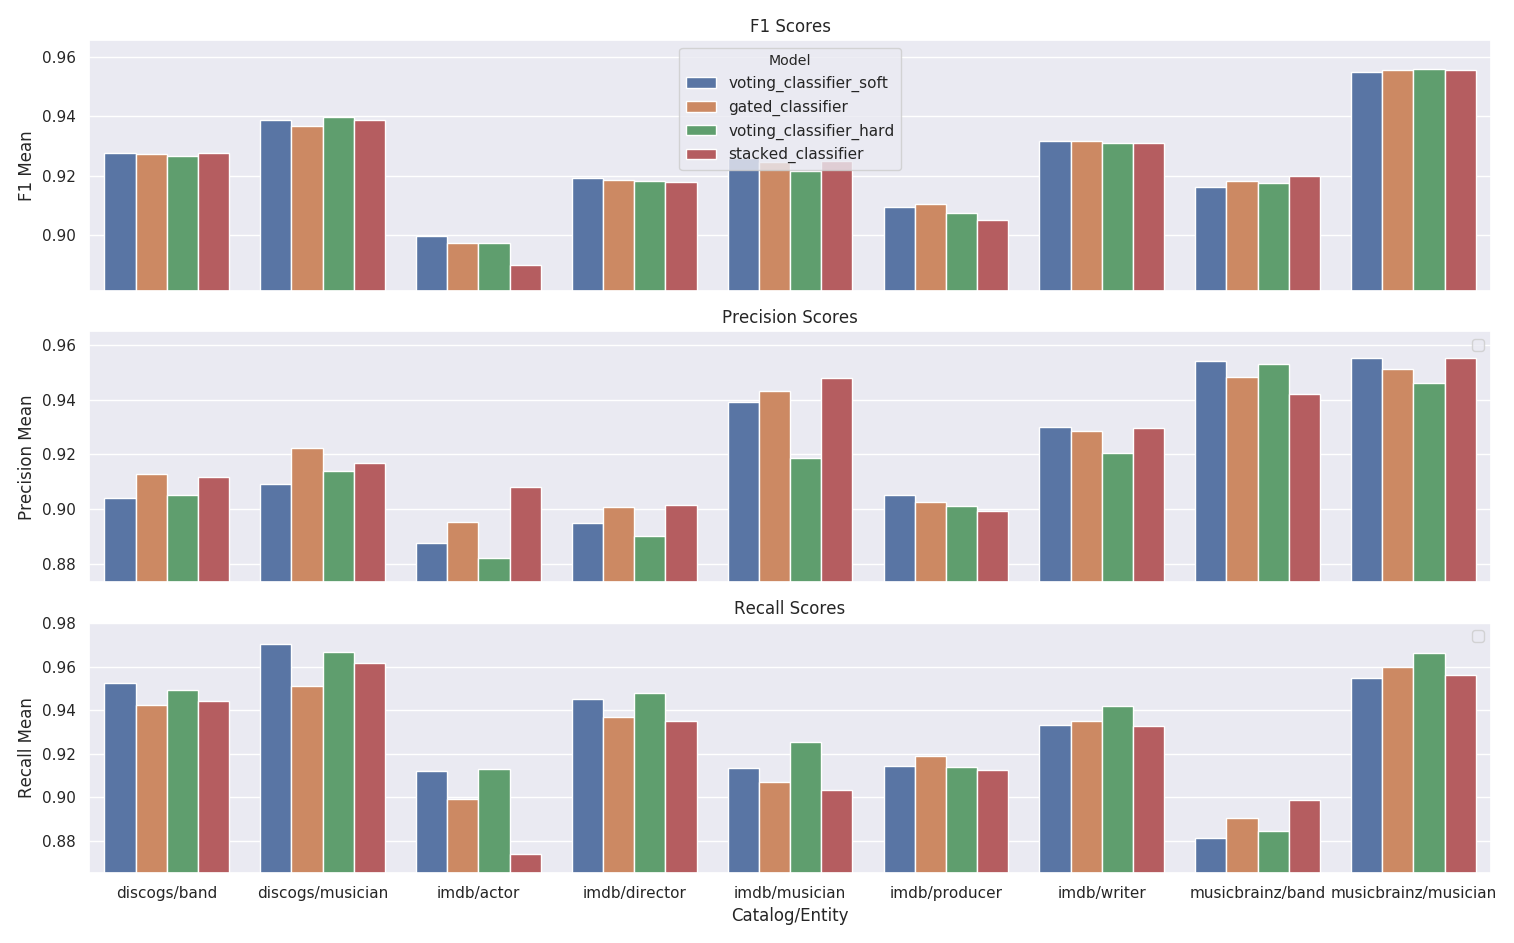
\includegraphics[width=\textwidth]{ensemble_evluation_main_metrics_barplot} 
  \caption{Barplots of the evaluation metrics for ensemble models. Separated by concrete entity.}
  \label{fig:ensmble-evaluation-barplots}
\end{figure}

In the figure above it can be better appreciated which classifiers performs best for which metrics. It is also clear which concrete entities are easier for the models to predict. As for the baseline models, it still appears that \textit{IMDb/Actor} is the hardest one to classify. Stack classifier seems to yield an acceptable precision for this concrete entity, however its recall is quite low. As with the baseline models, it can also be noted that \textit{Musicbrainz/Band} has a high precision and a low recall.  

The F1 scores are all similar when talking about the same concrete entity. The ones that show some more variation are \textit{IMDb/Actor} and \textit{IMDb/Producer}. 

As for recall, it can be clearly seen that in almost all cases the best models are one of the \textit{voting} classifiers. The only exception is for \textit{IMDb/Producer}, where \textit{Gated classifier} gives the best recall.

The table below has the average metrics that each classifier obtained for each catalog in general. These have been sorted by decreasing value of F1 score.

\begin{longtable}{|l|l|l|l|l|l|l|l|}
\hline
Catalog     & Model & Avg.F1   & Avg.F1.STD & Avg.Prec & Avg.Prec.STD & Avg.Rec  & Avg.Rec.STD \\ \hline
musicbrainz & sc    & 0.937717 & 0.002314   & 0.948661 & 0.007397     & 0.927434 & 0.008182    \\
musicbrainz & gc    & 0.936882 & 0.002871   & 0.949793 & 0.009169     & 0.925171 & 0.012389    \\
musicbrainz & vh    & 0.936772 & 0.001716   & 0.949564 & 0.005420     & 0.925423 & 0.004117    \\
musicbrainz & vs    & 0.935617 & 0.002162   & 0.954619 & 0.002448     & 0.918064 & 0.003565    \\ \hline
imdb        & vs    & 0.917241 & 0.001822   & 0.911329 & 0.006029     & 0.923645 & 0.005279    \\
imdb        & gc    & 0.916532 & 0.002469   & 0.913999 & 0.006489     & 0.919484 & 0.006835    \\
imdb        & vh    & 0.915104 & 0.002345   & 0.902533 & 0.009797     & 0.928480 & 0.009624    \\
imdb        & sc    & 0.913781 & 0.004725   & 0.917226 & 0.010621     & 0.911462 & 0.017587    \\ \hline
discogs     & sc    & 0.933304 & 0.001776   & 0.914405 & 0.004717     & 0.953101 & 0.006722    \\
discogs     & vs    & 0.933236 & 0.001397   & 0.906695 & 0.003530     & 0.961428 & 0.003844    \\
discogs     & vh    & 0.933226 & 0.001538   & 0.909535 & 0.002363     & 0.958201 & 0.002333    \\
discogs     & gc    & 0.932046 & 0.002087   & 0.917658 & 0.003622     & 0.946937 & 0.005928    \\ \hline
\end{longtable}


\begin{table}[H]
\centering
\begin{tabular}{l|l|l|l}
                                 & Best Avg.F1 & Best Avg.Prec & Best Avg.Rec \\ \hline
\multicolumn{1}{l|}{Musicbrainz} & sc          & vs            & sc           \\ \hline
\multicolumn{1}{l|}{IMDb}        & vs          & sc            & vh           \\ \hline
\multicolumn{1}{l|}{Discogs}     & sc          & gc            & vs           \\ 
\end{tabular}
\caption{Best performing ensemble models for each catalog according to the three main metrics.}
\label{tab:best-ensemble-model-per-metric-average}
\end{table}


There is no clear distinction about which is the best ensemble model. Both \textit{soft voting} and \textit{stack} classifier seem to have quite good performance. Stack classifier performs better for catalogs which have more information (Discogs and Musicbrainz), while soft voting performs best for IMDb that has less. 

Voting classifier appears to have the best precision for \textit{Musicbrainz}, however this is also the model which has the worst \textit{recall} for that catalog. On the other hand, \textit{stack classifier}, which is the best F1 and recall on this catalog, is also the one with the worst precision. 

For IMDb the best F1 score is given to \textit{soft voting}, which interestingly it is not the best at precision nor at recall, those places are given to \textit{stack} and \textit{hard voting} classifiers respectively. However, \textit{stack classifier} is the one with the worst recall, and \textit{hard voting} is the one with the lowest precision. For this catalog it can also be seen that the \textit{stack} classifier, which performs well for \textit{Musicbrainz} and \textit{Discogs} is actually the one with the worst F1 score.

The best F1 score for Discogs is given to the \textit{stack classifier}. Like in IMDb, this best F1 model actually does not have the best precision nor recall. Best precision is given by the \textit{gated classifier}, which is also the model with the worst recall and F1 score. \textit{Soft voting} classifier is the one which gives the best recall, and it also has the worst precision.

The table below shows a summary of the scores obtained by each model. These have been obtained by averaging all the model's scores. The rows are ordered by \textit{Avg. F1} in decreasing order. The best value for each metric is denoted in \textbf{bold}.

\begin{table}[H]
\centering
\begin{tabular}{l|l|l|l|l|l|l}
Model & Avg. F1  & Avg. F1.STD & Average Prec & Avg. Prec.STD & Avg. Recall & Avg. Recall.STD \\ \hline
vs    & \textbf{0.924879} & 0.001803    & 0.919919     & 0.004678      & \textbf{0.930801}    & 0.004579        \\
gc    & 0.924502 & 0.002473    & 0.922766     & 0.006448      & 0.926848    & 0.007868        \\
vh    & 0.923946 & 0.002026    & 0.914540     & 0.007172      & 0.934405    & 0.006780        \\
sc    & 0.923439 & 0.003534    & \textbf{0.923585}     & 0.008592      & 0.924264    & 0.013082          
\end{tabular}
\caption{Average metric score for each ensemble classifier.}
\label{tab:metrics-summary-for-ensembles}
\end{table}

From the results above it can be seen that both \textit{stack based} models have the best average precision. These are: \textit{gated classifier}, which has the best precision, and \textit{stack classifier}, which has the second best. On the other hand, \textit{voting based} classifiers have the best recall: \textit{hard voting}, which has the best recall, and \textit{soft voting} which has the second best.

\textit{Soft voting} also has the best precision when compared with \textit{hard voting}. Probably because soft voting considers an average of its base models predictions, so if a model is \textit{very} certain about a match then this amount will be taken into consideration for the final prediction. On the other hand, \textit{hard voting} only considers how many base models predicted a positive or negative, and not how certain they were about this prediction. 

An important thing to note in the table above is that \textit{soft voting} is also the classifier with the least standard deviation in all its metrics measurements. This means that the metrics obtained during the 5-fold cross validation did not change much across different folds, meaning that the final performance of the model is not that dependent upon the distribution of the data it was trained with. This is important since it gives more certainty that real world performance will be similar as that evaluated\footnote{If the classification data distribution is similar to that of the training set.}. 




\section{Comparative Evaluation}
\label{sec:comparative-evaluation}

The results showed in the previous two sections for baseline and ensemble models seem quite good. However, it still needs to be decided which technique has the overrall best performance, and, if possible, also define a classifier which can be said is the best among the pool of available classifiers. This section strives to answer these questions. 

The table below shows the best three models for each metric, each cell (which contains the model and their respective score for that metric) has been sorted in descending order. 

\begin{table}[H]
\centering
\begin{tabular}{|l|l|ll|ll|ll|}
\hline
Catalog                      & Entity                    & Model & F1.Mean  & Model & Prec.Mean & Model                & Recall.Mean \\ \hline
\multirow{6}{*}{di$sc^*$ogs}     & \multirow{3}{*}{band}     & $mlp^+$  & 0.928931 & $mlp^+$   & 0.915249  & $lsvm^+$                 & 0.956090    \\
                             &                           & $sc^*$    & 0.927771 & $gc^*$    & 0.912845  & $nb^+$                   & 0.955542    \\
                             &                           & $vs^*$    & 0.927576 & $sc^*$    & 0.911809  & $vs^*$                   & 0.952312    \\ \cline{2-8} 
                             & \multirow{3}{*}{musician} & $mlp^+$   & 0.940715 & $gc^*$    & 0.922472  & $lsvm^+$                 & 0.970741    \\
                             &                           & $vh^*$    & 0.939658 & $mlp^+$   & 0.921507  & $vs^*$                   & 0.970543    \\
                             &                           & $vs^*$    & 0.938896 & $slp^+$   & 0.917755  & $vh^*$                   & 0.966938    \\ \hline
\multirow{15}{*}{imdb}       & \multirow{3}{*}{actor}    & $vs^*$    & 0.899699 & $sc^*$    & 0.907933  & $nb^+$                   & 0.963789    \\
                             &                           & $rf^+$    & 0.899161 & $gc^*$    & 0.895105  & $rf^+$                   & 0.919592    \\
                             &                           & $gc^*$    & 0.897257 & $vs^*$    & 0.887665  & $mlp^+$                  & 0.913832    \\ \cline{2-8} 
                             & \multirow{3}{*}{director} & $mlp^+$   & 0.919340 & $sc^*$    & 0.901563  & $nb^+$                   & 0.967075    \\
                             &                           & $vs^*$    & 0.919262 & $gc^*$    & 0.900678  & $vh^*$                   & 0.947915    \\
                             &                           & $gc^*$    & 0.918505 & $mlp^+$   & 0.899994  & $lsvm^+$                 & 0.947397    \\ \cline{2-8} 
                             & \multirow{3}{*}{musician} & $vs^*$    & 0.926019 & $sc^*$    & 0.947724  & $nb^+$                   & 0.948158    \\
                             &                           & $mlp^+$   & 0.925888 & $gc^*$    & 0.943199  & $lr^+$ & 0.927680    \\
                             &                           & $sc^*$    & 0.924930 & $mlp^+$   & 0.942860  & $lsvm^+$                 & 0.926534    \\ \cline{2-8} 
                             & \multirow{3}{*}{producer} & $gc^*$    & 0.910555 & $vs^*$    & 0.905090  & $nb^+$                   & 0.962525    \\
                             &                           & $vs^*$    & 0.909610 & $slp^+$   & 0.903146  & $mlp^+$                  & 0.925119    \\
                             &                           & $mlp^+$   & 0.909398 & $gc^*$    & 0.902453  & $gc^*$                   & 0.918955    \\ \cline{2-8} 
                             & \multirow{3}{*}{writer}   & $gc^*$    & 0.931719 & $vs^*$    & 0.929887  & $nb^+$                   & 0.965145    \\
                             &                           & $vs^*$    & 0.931617 & $sc^*$    & 0.929588  & $vh^*$                   & 0.942038    \\
                             &                           & $vh^*$    & 0.931065 & $gc^*$    & 0.928561  & $lsvm^+$                 & 0.938421    \\ \hline
\multirow{6}{*}{musicbrainz} & \multirow{3}{*}{band}     & $mlp^+$   & 0.921134 & $lsvm^+$  & 0.961199  & $mlp^+$                  & 0.915818    \\
                             &                           & $sc^*$    & 0.919791 & $vs^*$    & 0.954029  & $rf^+$                   & 0.900192    \\
                             &                           & $rf^+$    & 0.918844 & $vh^*$    & 0.953082  & $lr^+$                   & 0.899217    \\ \cline{2-8} 
                             & \multirow{3}{*}{musician} & $mlp^+$   & 0.957375 & $sc^*$    & 0.955374  & $mlp^+$                  & 0.971004    \\
                             &                           & $vh^*$    & 0.956088 & $vs^*$    & 0.955208  & $vh^*$                   & 0.966356    \\
                             &                           & $sc^*$    & 0.955643 & $nb^+$    & 0.953561  & $lsvm^+$                 & 0.966225    \\ \hline
\end{tabular}
\caption{Best three models and their scores for each respective metric. These results are shown for each concrete entity. To better differentiate the provenance of the each classifier, their names have been super-scripted with a $^+$ if they are models from the baseline, while those symbolizing ensemble models were super-scripted with $^*$}
\label{tab:comparison-bl-ens-top-3}
\end{table}


It can be noticed that in almost all cases, the list of \textit{top 3} models for each metrics includes both classifiers coming from the set of baseline classifiers as well as ensemble classifiers. The exceptions for this are \textit{Precision} for \textit{IMDb/Actor}, where the list of top-3 is composed only of ensemble models. The \textit{Recall} for the same model, and for \textit{Musicbrainz/Band} is instead composed only of baseline models. The list for \textit{Recall}, for \textit{IMDb/Musician} is also composed of only baseline classifiers. All classifiers in the lists for \textit{F1 score} and \textit{precision} of \textit{IMDb/Writer} are exclusively from the set of ensemble classifiers.

The pie plots below show the number of times each model appeared in the first, second, or third positions. 

\begin{figure}[H]
  \centering 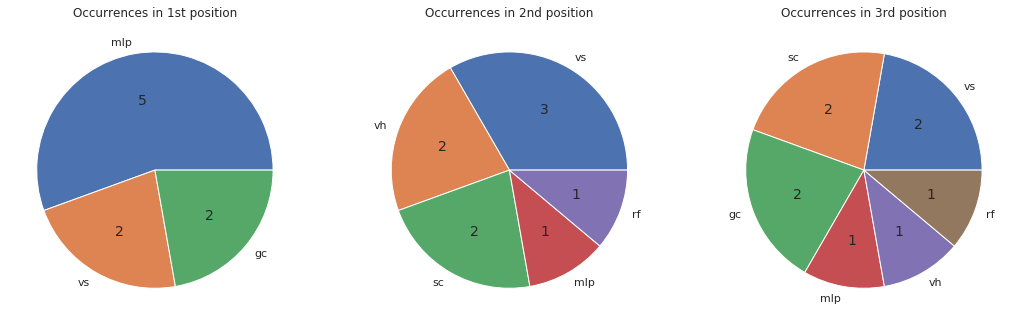
\includegraphics[width=\textwidth]{comparison_f1_top_spaces_pies} 
  \caption{Pie plots show the occurrences of each model in each position of the \textit{top 3}, for the F1 metric.}
  \label{fig:comparison-pie-occurrences-f1}
\end{figure}

\begin{figure}[H]
  \centering 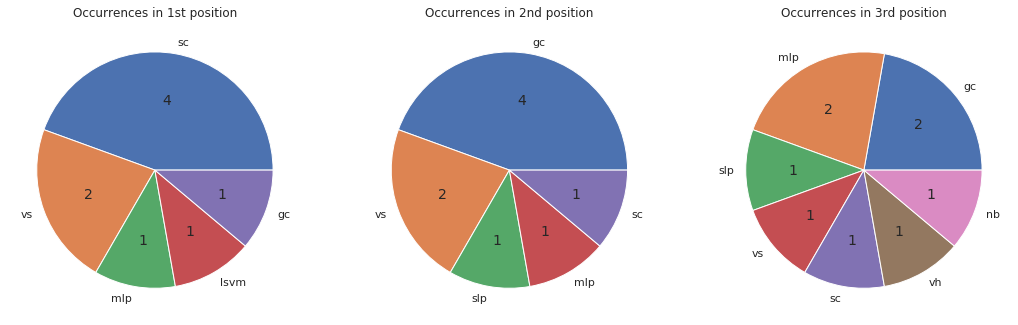
\includegraphics[width=\textwidth]{comparison_prec_top_spaces_pies} 
  \caption{Pie plots show the occurrences of each model in each position of the \textit{top 3}, for the \textit{Precision} metric.}
  \label{fig:comparison-pie-occurrences-precision}
\end{figure}

\begin{figure}[H]
  \centering 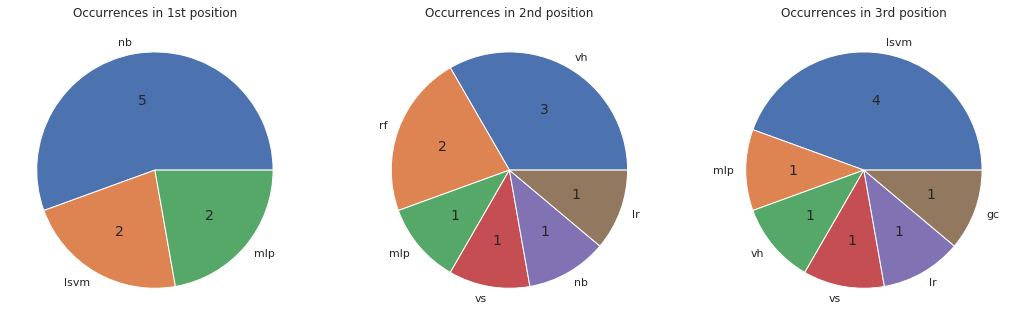
\includegraphics[width=\textwidth]{comparison_recall_top_spaces_pies} 
  \caption{Pie plots show the occurrences of each model in each position of the \textit{top 3}, for the \textit{Recall} metric.}
  \label{fig:comparison-pie-occurrences-recall}
\end{figure}

It can be seen in \autoref{fig:comparison-pie-occurrences-f1} that \textit{mlp} appears as the model with the highest score more than half the time. Followed by \textit{soft voting} and \textit{gate classifier}, which both appear in two of the cases. Soft voting is also the model which appears more time in as the second best F1. Both \textit{mlp} and \textit{vs} appear among the top-3 for F1 in 7 out of the nine cases.

\autoref{fig:comparison-pie-occurrences-precision} shows the occurrences for the precision metric. Here it can be see that ensemble based classifiers appear a total of 7 times out of 9 as the top-1 model: \textit{stack classifier} appears 4 times, \textit{soft voting} appears 2, and \textit{gated classifier} appears once. The baseline models which appear as top-1 once each are \textit{mlp} and \textit{lsvm}. Something similar happens for the model which appears in the second place: 7 times out of 9 there is an ensemble model (4 times \textit{gc}, 2 times \textit{vs}, and once \textit{sc}), while the remaining two spots are taken by \textit{mlp} and \textit{slp}. 

For the recall case, in \autoref{fig:comparison-pie-occurrences-recall}, in can be seen that there are no cases where an ensemble classifier appears as the one with the best score. It seems that the the best recall is given to \textit{nb}, which appears as top-1 5 out of 9 times, and \textit{lsvm} and \textit{mlp} which appear twice each. It can be seen that in the second best recall spot there are ensemble models. 4 our of the 9 cases for this second spot are taken by ensemble classifiers (3 times \textit{vh}, and once \textit{vs}). 

Note that even though \textit{naive bayes} appears in the first and second places for recall, it does not appear as one of the top 3 for any of the other metrics, except for the one time it appears in the third position for precision. It is also interesting to notice that \textit{stack classifier}, which is the one which most commonly appears as top precision, does not appear even once among the top 3 recalls.

From the above it can be seen that ensemble models tend to have a higher precision than baseline models. However, they also have a lower recall. A pattern also seems to be emerging in regards to which models appear as the best. For instance, it can be said that both \textit{mlp} and \textit{vs} have good performance in most of the cases. Also, it seems that ensemble models perform better, more commonly, than baseline classifiers. The exception is \textit{mlp}, which appears to perform best in some cases.

The table below shows the average metrics obtained for the top 5 models, ordered in descending order by F1 score. 

\begin{table}[H]
\centering
\begin{tabular}{l|l|l|l|l|l|l}
Model & Avg.F1       & Avg.F1.STD & Avg.Prec     & Avg.Prec.STD & Avg.Recall   & Avg.Recall.STD \\ \hline
mlp   & 0.925556 (1) & 0.001667   & 0.916643 (4) & 0.003465     & 0.934975 (1) & 0.003420       \\
vs    & 0.924879 (2) & 0.001803   & 0.919919 (3) & 0.004678     & 0.930801 (3) & 0.004579       \\
gc    & 0.924502 (3) & 0.002473   & 0.922766 (2) & 0.006448     & 0.926848 (4) & 0.007868       \\
vh    & 0.923946 (4) & 0.002026   & 0.914540 (5) & 0.007172     & 0.934405 (2) & 0.006780       \\
sc    & 0.923439 (5) & 0.003534   & 0.923585 (1) & 0.008592     & 0.924264 (5) & 0.013082      
\end{tabular}
\caption{Average metrics for top-5 models ordered by F1 score. The parenthesis to the right of the average scores show the respective position to respect to the other values of that same score. }
\label{tab:comparison-average-all-models}
\end{table}

In the table above it can be clearly seen that \textit{mlp} is the best performing classifier when it comes to \textit{average F1}, and is also the model with the best \textit{average recall}. However, \textit{mlp} is also the model with the second worst precision (\textit{vh} is the model with the worst precision). 
 
Another interesting thing to notice is that in this table, \textit{mlp} is the only baseline model in the top-5. Notice also the standard deviations, \textit{ensembles} seem to have higher values for all metrics than \textit{mlp}. 

Now the question arises of whether these averages actually tell the behaviour of the algorithm, or whether some of the algorithms had a very good performance for one of the catalog entities. This behaviour can be better seen in the next figure.

\begin{figure}[H]
  \centering 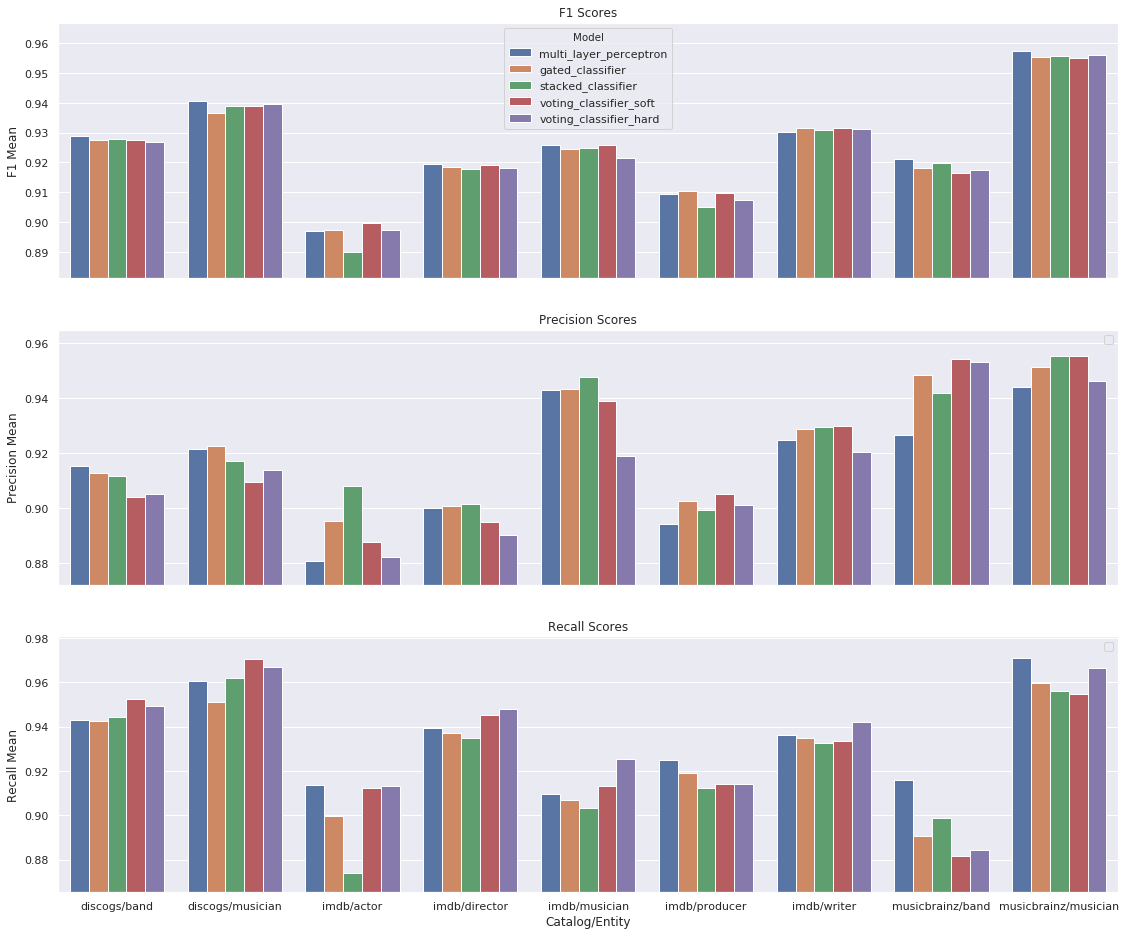
\includegraphics[width=\textwidth]{comparison_barplots_all_metrics} 
  \caption{Barplot showing the metrics obtained by all top-5 classifiers.}
  \label{fig:comparison-barplot-all-metrics}
\end{figure}

In the figure above it can be clearly appreciated the the F1 scores are almost always similar, except for the \textit{Musicbrainz} entities, where \textit{mlp} clearly performs better. For \textit{IMDb/Actor}, which has been shown to be problematic for all models to classify in the previous two sections, \textit{mlp} does not perform very well, instead the best scores are obtained for \textit{vs} and \textit{gc}.

For the precision values, ensemble models seem to be more consistent, especially \textit{stack classifier}. The precision of \textit{mlp} is high for some concrete entities (e.g. \textit{Discogs/Band}), but it is actually lower than for the other models for most other entities (e.g. both \textit{Musicbrainz} entities). This result was, however, already expected from what was shown in \autoref{tab:comparison-bl-ens-top-3}.

For recall, all models seems to perform quite similarly. The exceptions are for entities of the \textit{Musicbrainz} catalog, where \textit{mlp} has a much higher recall than the ensemble models, which may also explain why it has a higher F1 for this same entities even if its precision is not that good.

It is interesting that the performance of \textit{mlp} is better for recall and F1, considering that the ensembles actually have a \textit{mlp} as one of their base model. Some reasons for this may be that there are some classifiers among the base models which are producing more noise than actually useful prediction. 

For example, one of the least performing baseline models, specifically those with low recall, like \textit{slp} may be driving the ensemble to make some predictions which cause it to miss-classify some \textit{positive} examples, and as such decreasing the overrall recall. A more careful selection of the base models may help to solve these issues by only including models which are helpful for the ensemble.


\chapter{Conclusion}
\label{chap:conclusion}

\todo[inline,color=green!25]{Work in progress}

Ensembles have better precision but tend to have a lower recall. Because of this their F1 suffers, and as such they do not manage to get the top score for this metric. However, if the situation we're currently in values precision above recall, ensemble models are the best choice.

As seen in the results comparison section, the \textit{multi-layer perceptron} performs well in most cases, and the aggregated complexity of training an ensemble of models may not be worth it even if they do provide a higher precision. Obviously, the decision of whether this is worth or not must be taken on a per problem basis. Besides this, 4 out of the 5 models with best F1 score, presented in the last section, are ensemble models, showing that they're still better than most baseline models.

Even though the performance of the ensembles in terms of \textit{F1} and \textit{recall}, was not the best, they did show a very good precision. Meaning that the mixing of opinions from its base classifiers actually supplies valuable information to the prediction process, and makes it more sensitive to \textit{negative} samples. Some their application may make more sense if the problem currently being worked on does not tolerate \textit{false positives}.

Another thing that should be kept in mind is that the results presented for the ensemble models are for ensemble who use as their base classifiers all models available in the baseline. This might not actually be optimal, and as said in the previous section, there may be some models which are driving the ensembles to make miss-predictions. A more careful construction of the base model set may improve the final performance of the ensembles. 

% - maybe write something about what was expected and if this was attained or not. And why not or yes
% - 


\section{Future Work}
\label{sec:future-work}

Other things that might still be done to improve the project.

It would be a good idea to use one of the collective matching methods
\cite{Dong2005_reference_reconciliation,bhattacharya07_collec_entit_resol_relat_data,Kalashnikov2006_collective_graph}
to leverage the information of composed entities. For example, in the current
data we know that \textit{actors} are part of \textit{movies}, and that
\textit{musicians} are part of \textit{bands}. The similarity among
\textit{actors}/\textit{musicians} may be dependent upon the similarity of the
movies in which they appear, or the bands in which they have performed.

% ---
better selection of base models may reduce noise in ensembles and improve final performance. 
% ---
It would be interesting to see how the performance would vary if new catalogs were to be added.
% ---
There are also other assembling approaches that weren't explored to maintain the scope of the thesis manageable (ie, boosting, bayesian record linkage.)
% ---


%%%%%%%%%%%%%%%%%%%%%%%%%%%%%%%%%%%%%%%%% 
\endgroup


bibliografia in formato bibtex
     
% aggiunta del capitolo nell'indice
\addcontentsline{toc}{chapter}{Bibliography}
% stile con ordinamento alfabetico in funzione degli autori
\bibliographystyle{plain} \bibliography{biblio}



\titleformat{\chapter} {\normalfont\Huge\bfseries}{Apendix \thechapter}{1em}{}
% sezione Allegati - opzionale
\appendix
\chapter{Appendix}

\subsection{Glossary}
\label{sec:apx-glossary}

This section will review the terminology which is extensively used in this work when talking about data and it's sources.

\subsubsection{Entity}
\label{sec:rl-term-entity}

An entity refers to a single data point in a dataset (catalog). \textit{Entities} are what is matched when performing record linkage. An entity is composed of one identifier, and a collection of fields (either quantitative or qualitative) which are specific to each problem. 
  
In the people use case, the entities will most likely have fields representing personal information \textit{(name, birth date, death date, etc.)}. If, on the other hand there is a problem where its necessary to perform record linkage on houses, then it would probably have fields like \texttt{total area, number of floors, number of rooms, etc}.


\subsubsection{Catalog}
\label{sec:rl-term-catalog}

In the present work, any source of entities is called a \textit{catalog}. The terms \textit{catalog} and  \textit{dataset} are synonyms. Any source of data can be a catalog: books, databases, spreadsheets, etc. 

Note that the term \textit{catalog} is not specific to Record Linkage. It is instead a term adopted from the Mix'n'Match\footurl{https://tools.wmflabs.org/mix-n-match} project, and it signifies \textit{sources of data which can be imported into Wikidata}. For our project, the term is changed slightly to mean \textit{any source of data}. 

An \textit{external catalog} is a \textit{catalog} that is not \textit{Wikidata}, and from which information should be imported into the latter.

As stated before, entities are always assigned an identifier. This said identifier is always unique, and specific to a distinct catalog (rarely this identifier is shared among different catalogs). 

When performing record linkage, it is desirable to end up with a list of identifiers pairs, where each pair describes a single real-world entity, and its identifiers tells us which record in the corresponding dataset has information on the specific entity.


\subsubsection{Source and Target}
\label{sec:rl-term-source-and-target}

As stated before, the goal is to take Wikidata entities and find their corresponding links in external catalogs. The relation between these two can be captured by the terms \textit{source} and \textit{target}. \textit{Source} is the catalog where the entities that should be matched are taken from (i.e. \textit{Wikidata}), and \textit{target} is the catalog against which the entities from the source should be matched (i.e. the external catalogs).

This is especially useful when there is no need to match all the catalogs amongst
themselves, since matching a \textit{source catalog} against multiple target ones
requires a much more diminished number of comparisons than it would do if matching all catalogs among themselves.

When using a \textit{source catalog}, the record linkage algorithm is no longer matching
source entities into a unique latent (underlying) entity, rather, it will match
them against a concrete entity (e.g. an entity from the source catalog).

In related record linkage studies, these terms are also commonly referred to as \cite{Sayers2015}
\textit{master file} (instead of source), and \textit{file of interest} (instead
of target) .
   

\section{Mapping IMDb Professions to Wikidata}
\label{sec:imdb-profs-to-wikidata}

\todo[inline,color=red!25]{Possibly this will be removed}

almost everything said in https://github.com/Wikidata/soweego/issues/165


\section{Distribution of features}
\label{sec:apx-feature-distribution}

\todo[inline,color=red!25]{Possibly this will be removed, features are already explained in their own section, and distplots do not add much information}


This section contains the plots which characterize the distributions of feature values extracted for different concrete entities. 

\autoref{fig:distribution-of-classification-features-1} and \autoref{fig:distribution-of-classification-features-2} present the distribution plot of features in the classification set. While \autoref{fig:distribution-of-training-features-1} and \autoref{fig:distribution-of-training-features-2} presents the distribution for the training set.

\autoref{fig:distribution-of-training-negative-features-1} and \autoref{fig:distribution-of-training-negative-features-2} show the distribution for features of negative samples from the training set. While \autoref{fig:distribution-of-training-positive-features-1} and \autoref{fig:distribution-of-training-positive-features-2} show those for the positive samples.

By comparing the classification and training sets one of the first things that can be noticed is that for features in all cases there is one feature which is almost always one, while in the classification set this happens only in some cases. The featrures with this behaviour are one of the \textit{exact measures}: \textit{exact anmes}, \textit{exact url}.

It is also interesting to note that in most plots, but especially in those for the classification set, the majority of the features values seem to be below \textit{0.7}.

For the training set distributions there is a bit more variations, and feature values are also higher feature values are more common. Here it can be noted that the \textit{exact} features are much more prominent than in the classification set. 

Comparing the positive and negative training distributions one can notice that for the positive distributions, in all cases, the exact matches measures are much higher than the others.

\todo[inline]{finish or remove section. exact measures squash all the others, but removing them would mean they should be presented in some other way.. might leverage the already presented table of percentages of zero values, the complement is the percentage of 1s (since exact is only 1/0)}

\begin{figure}[H]
  \centering 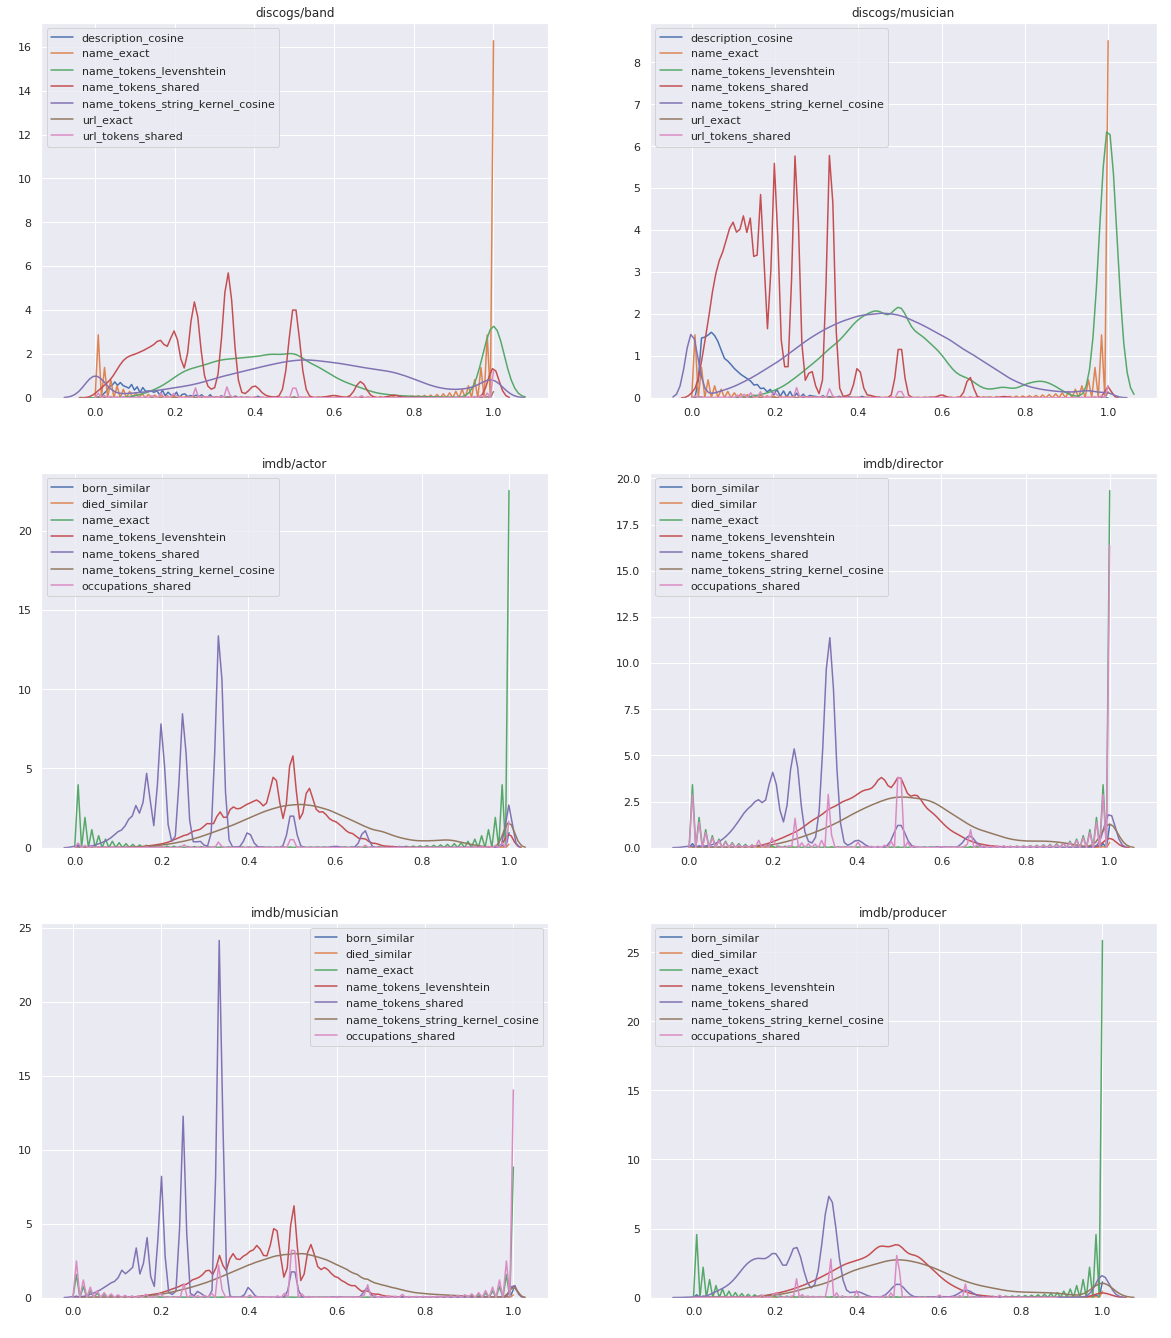
\includegraphics[width=\textwidth]{classification_feature_distribution} 
  \caption{Feature distribution for the classification set.}
  \label{fig:distribution-of-classification-features-1}
\end{figure}

\begin{figure}[H]
  \centering 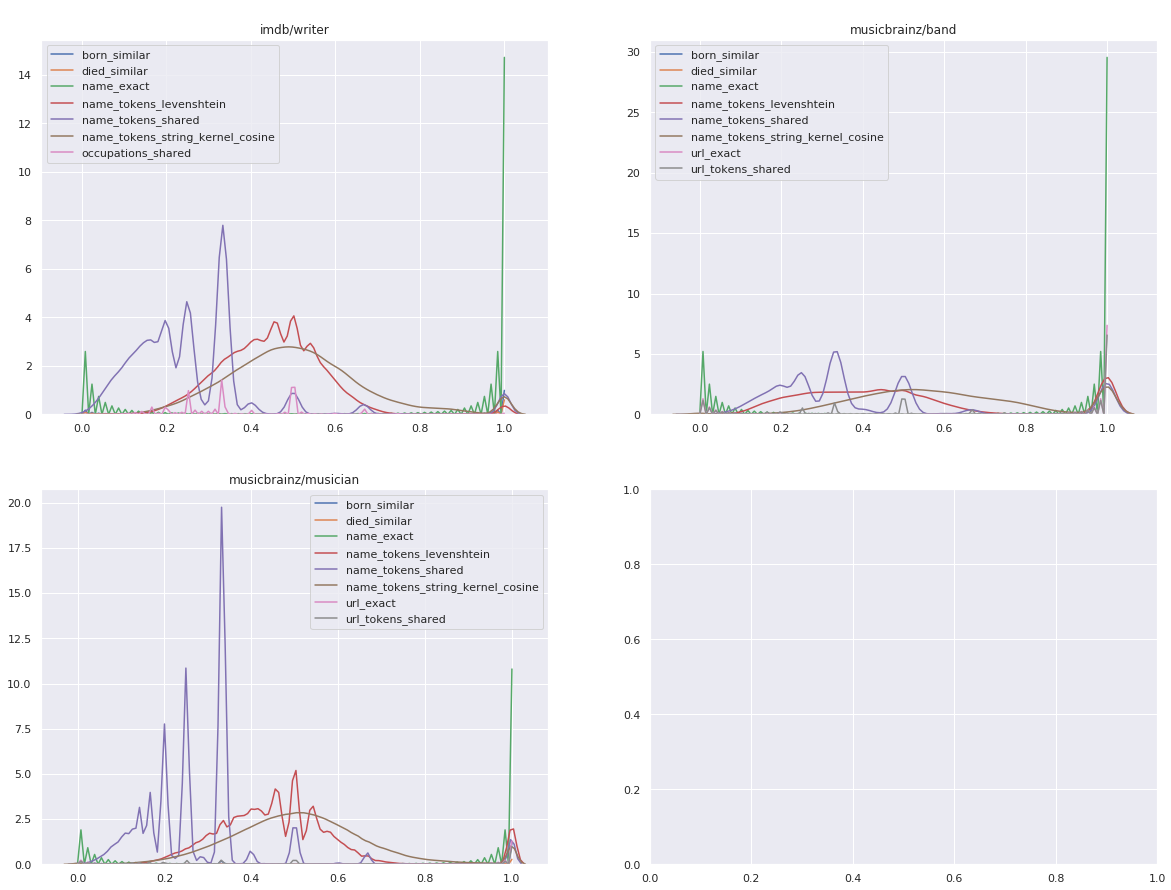
\includegraphics[width=\textwidth]{classification_feature_distribution_2} 
  \caption{Feature distribution for the classification set.}
  \label{fig:distribution-of-classification-features-2}
\end{figure}

\begin{figure}[H]
      \centering
      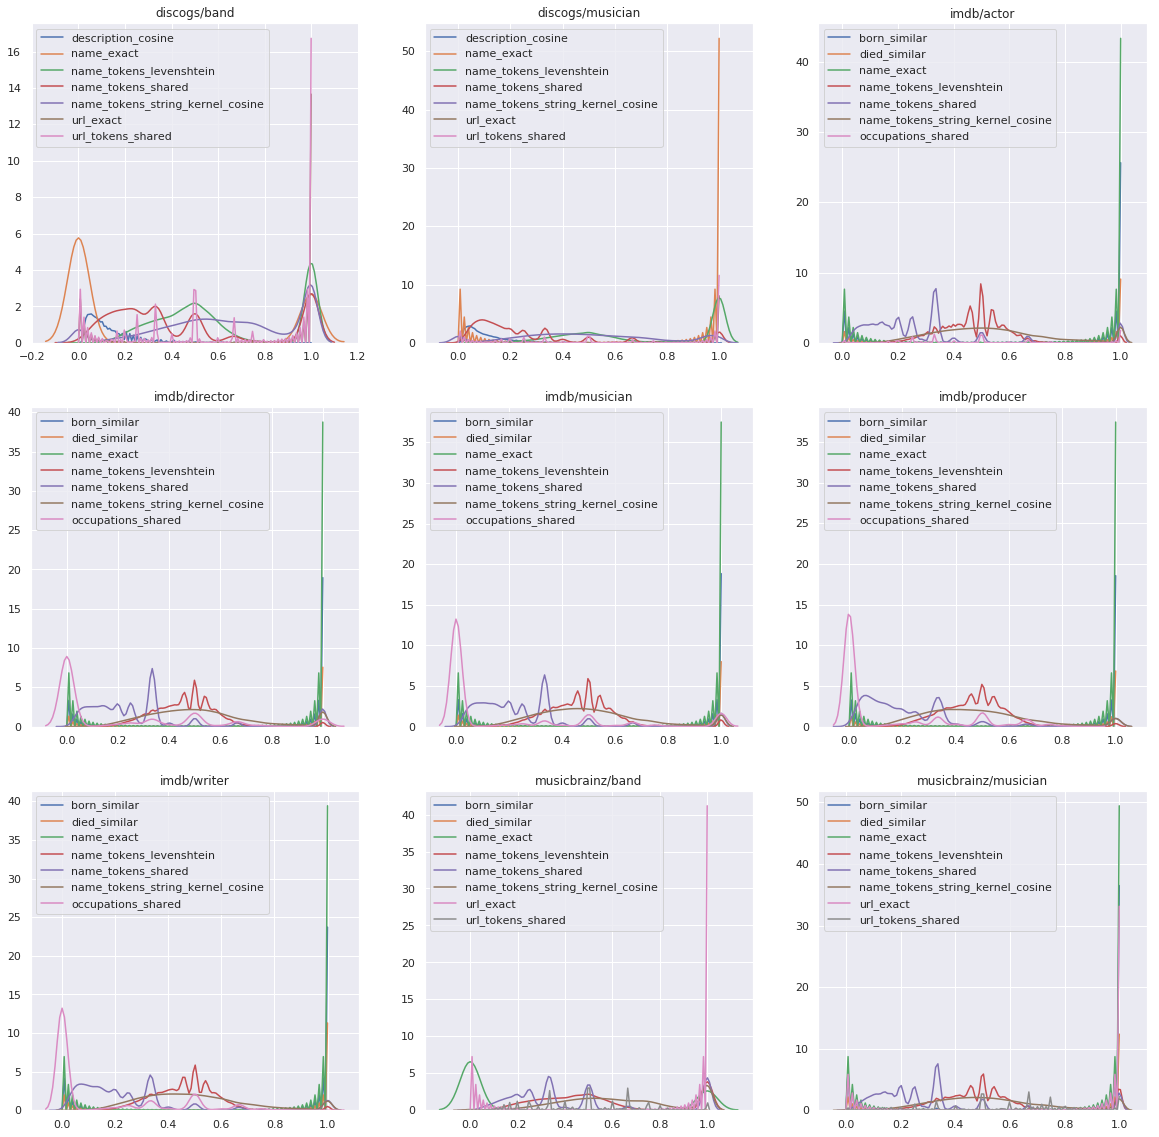
\includegraphics[width=\linewidth]{training_feature_distribution}
      \caption{Feature distribution for the training set (1).}
      \label{fig:distribution-of-training-features-1}
\end{figure}

\begin{figure}[H]
      \centering
      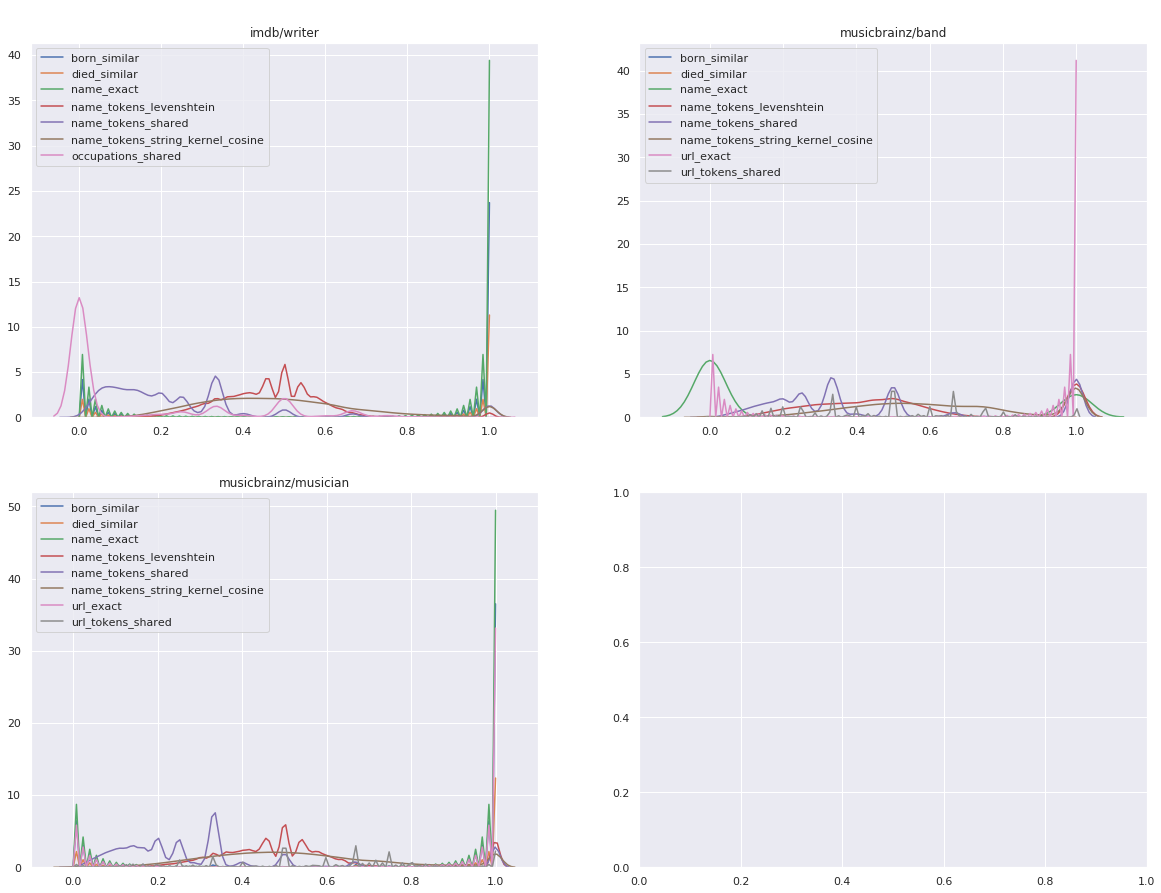
\includegraphics[width=\linewidth]{training_feature_distribution_2}
      \caption{Feature distribution for the training set (2).}
      \label{fig:distribution-of-training-features-2}
\end{figure}



\begin{figure}[H]
      \centering
      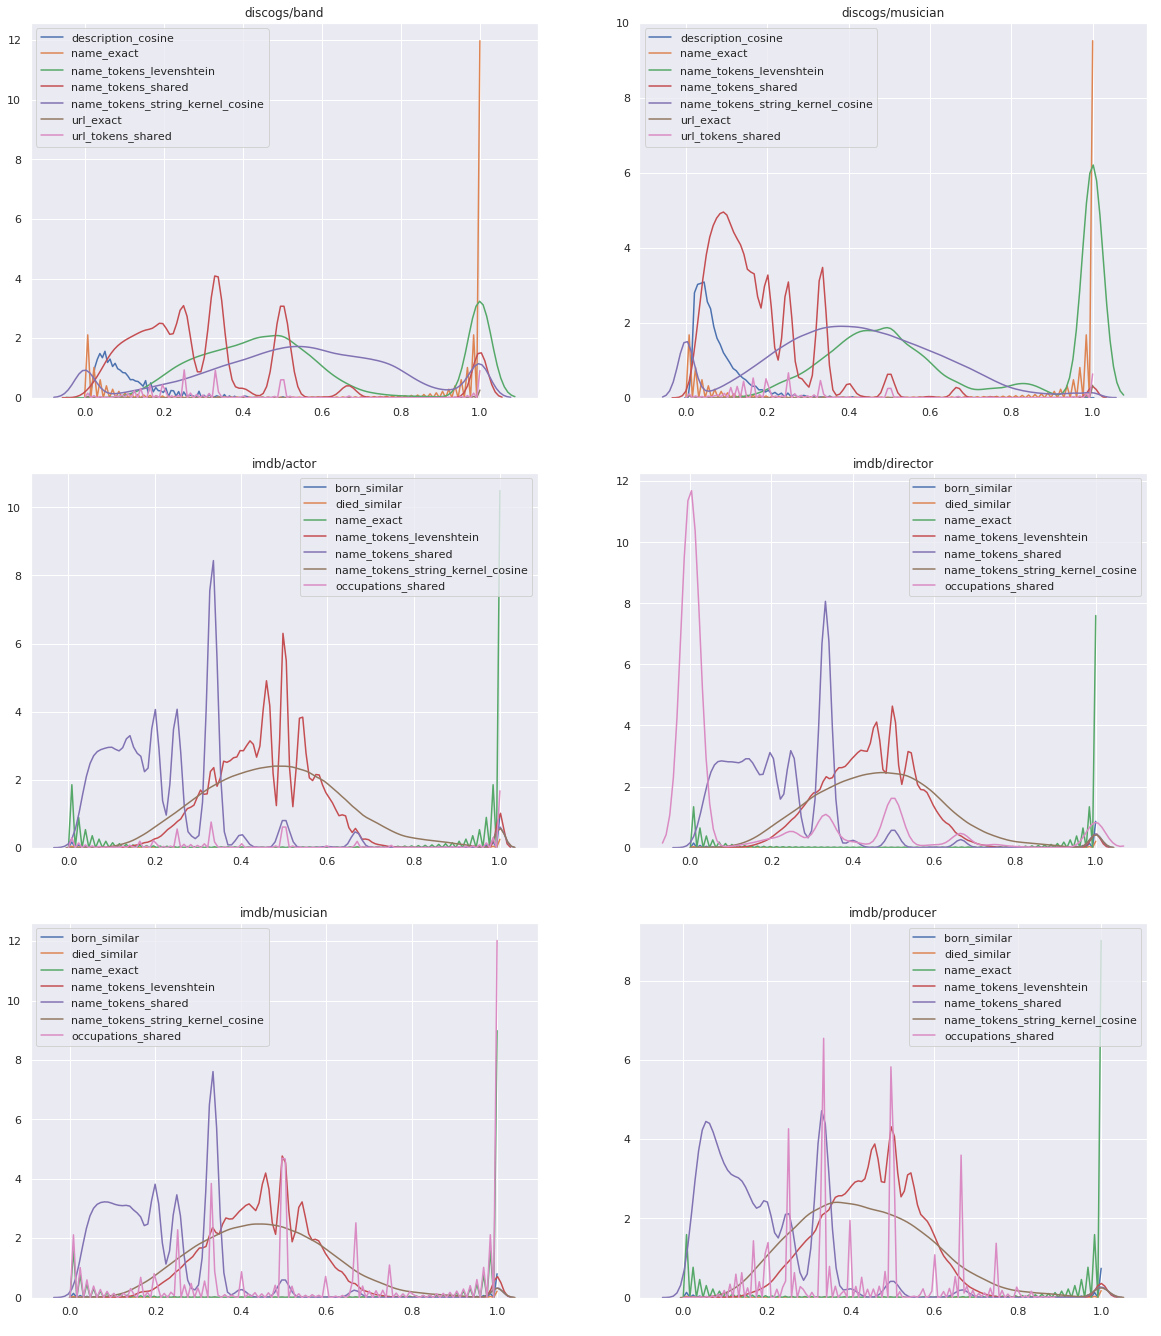
\includegraphics[width=\linewidth]{features_distribution_negative_samples_1}
      \caption{Feature distribution for the negative samples of the training set (1).}
      \label{fig:distribution-of-training-negative-features-1}
\end{figure}

\begin{figure}[H]
      \centering
      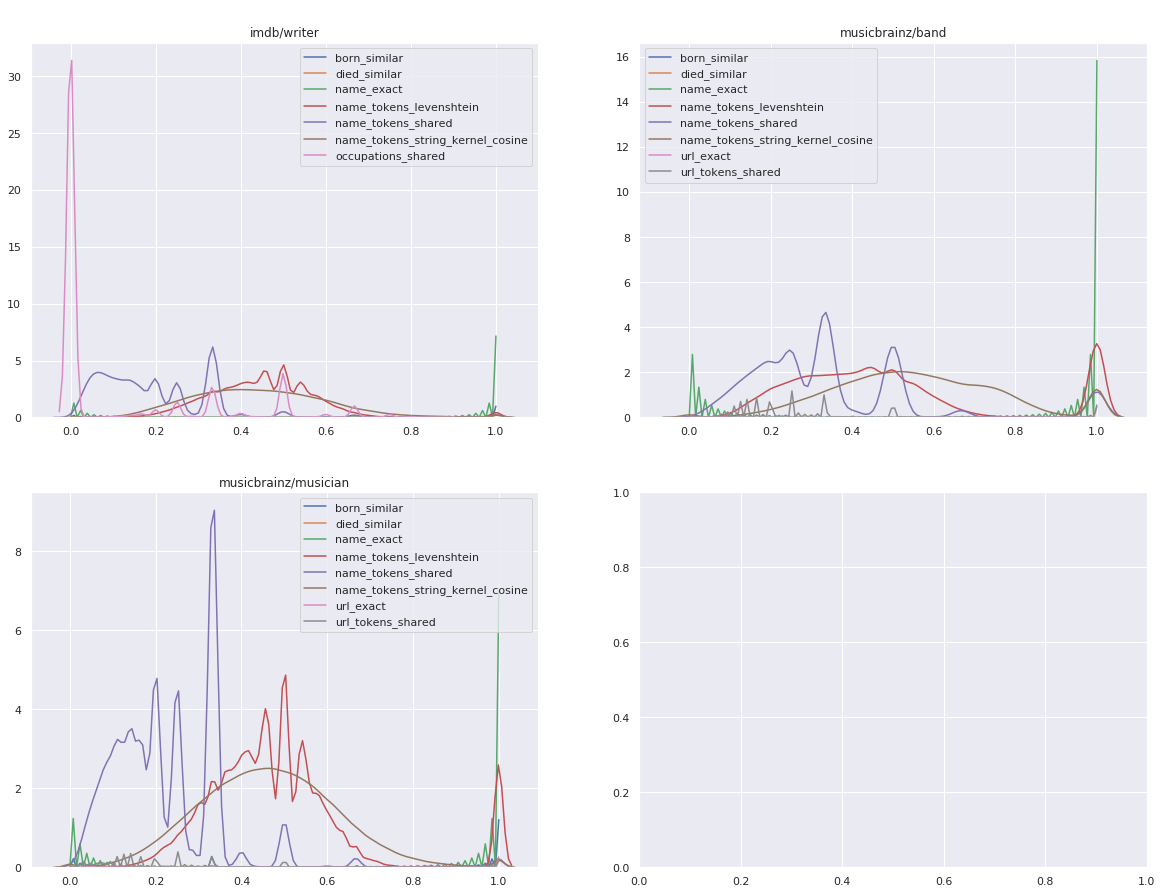
\includegraphics[width=\linewidth]{features_distribution_negative_samples_2}
      \caption{Feature distribution for the negative samples of the training set (2).}
      \label{fig:distribution-of-training-negative-features-2}
\end{figure}



\begin{figure}[H]
      \centering
      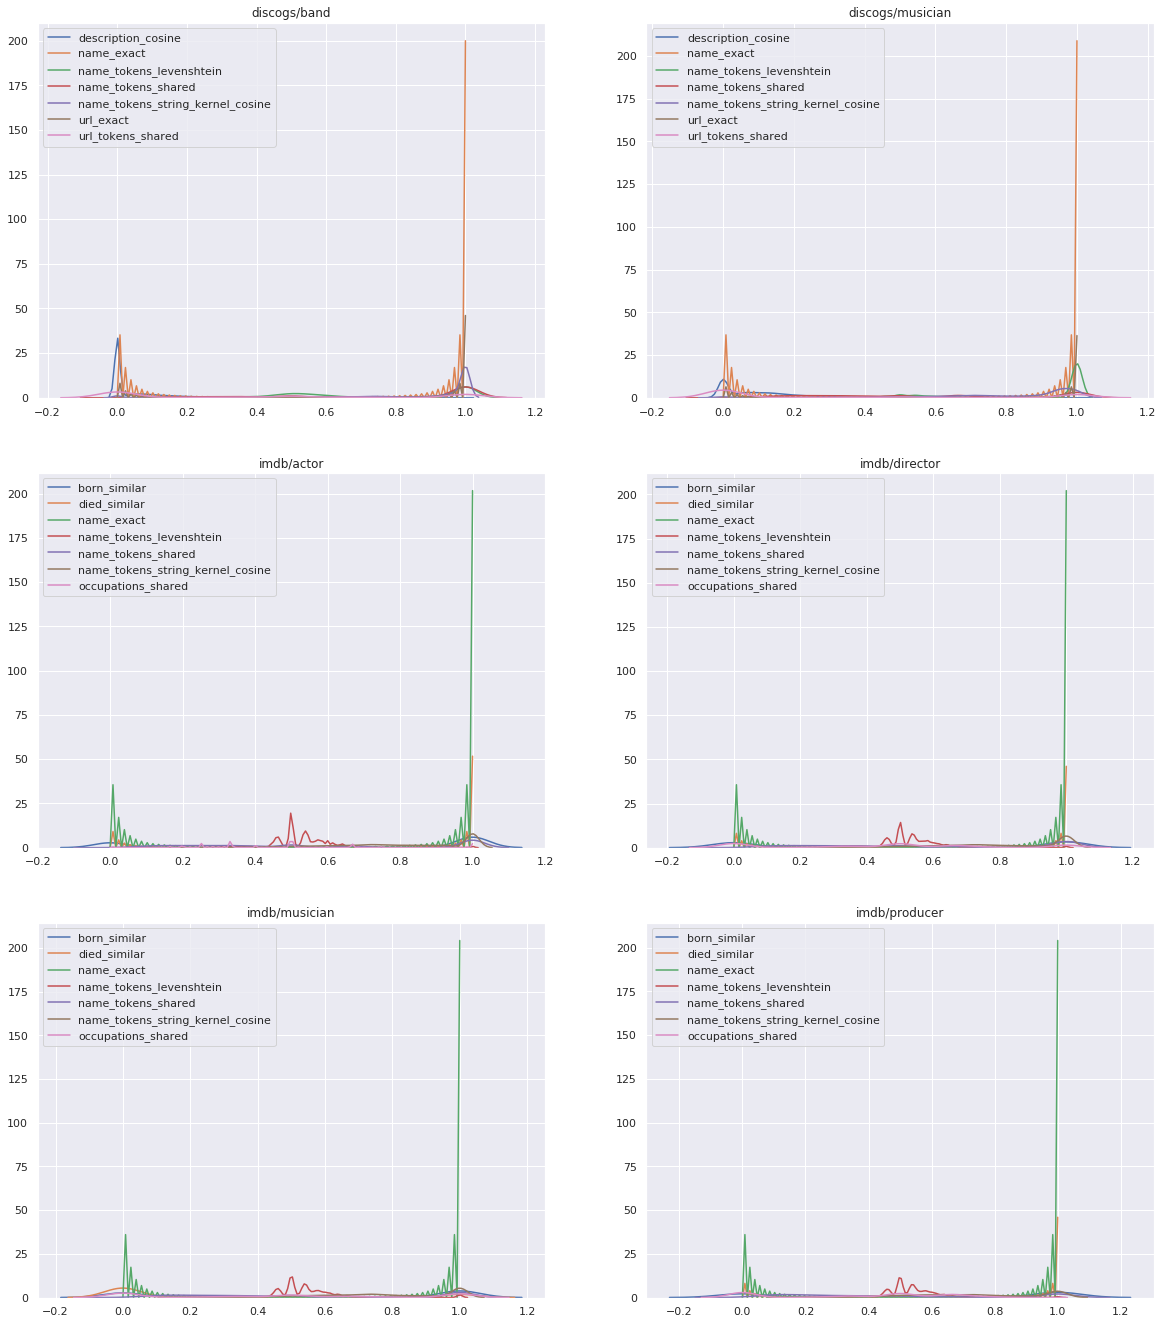
\includegraphics[width=\linewidth]{features_distribution_positive_samples_1}
      \caption{Feature distribution for the positive samples of the training set (1).}
      \label{fig:distribution-of-training-positive-features-1}
\end{figure}

\begin{figure}[H]
      \centering
      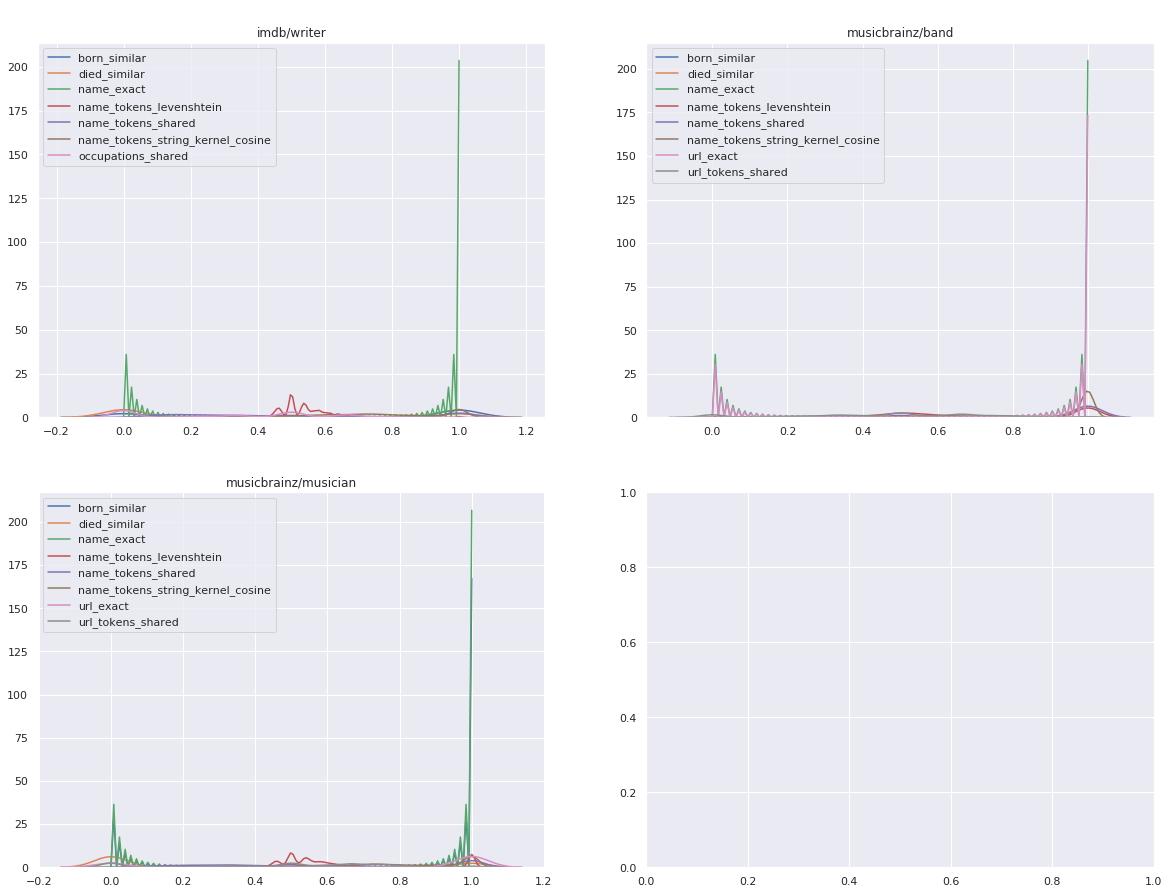
\includegraphics[width=\linewidth]{features_distribution_positive_samples_2}
      \caption{Feature distribution for the positive samples of the training set (2).}
      \label{fig:distribution-of-training-positive-features-2}
\end{figure}

\section{Analysis of classification distributions}
\label{sec:apx-classification-results}

\todo[inline,color=red!25]{Possibly this will be removed. Discussion on classification distribution does not add much if we don't know the labels}


When a classifier predicts if a pair is a match or not it will yield a prediction which may be between 0 and 1. This predictions can be plotted with a distribution plot to see how different classifiers behave for the same concrete entity.

This section contains the results of running the \texttt{soweego} pipeline on each concrete entity. The data used to create these results were the Wikidata training and classification dumps, and also the dumps for the external catalogs mentioned in \autoref{sec:orig-shape-of-data}. The training data was used for training each model, and the results were obtained from the classification data.

The following sections will show the results obtained for the baseline and ensemble models separately.

\subsection{Baseline classification results}
\label{sec:apx-baseline-classification-results}

The table below shows statics on the 

\begin{table}[H]
\centering
\begin{tabular}{|l|l|l|l|ll|l|}
\hline
Model                             & Average Mean & Average STD & Average 25\% & Average 50\% & Average 75\% & Average Max \\ \hline
single\_layer\_perceptron         & 0.911712     & 0.213713    & 0.963896     & 0.997227     & 0.998371     & 0.999749    \\
multi\_layer\_perceptron          & 0.911148     & 0.212020    & 0.945349     & 0.999371     & 0.999781     & 0.999994    \\
naive\_bayes                      & 0.077806     & 0.183952    & 0.000463     & 0.003623     & 0.078400     & 0.999998    \\
linear\_support\_vector\_machines & 0.057549     & 0.225727    & 0.000000     & 0.000000     & 0.000000     & 1.000000    \\
random\_forest                    & 0.053097     & 0.173311    & 0.000000     & 0.000000     & 0.000444     & 1.000000    \\
logistic\_regression              & 0.051562     & 0.162769    & 0.001627     & 0.002700     & 0.005134     & 0.999925    \\ \hline
\end{tabular}
\caption{}
\label{tab:my-table}
\end{table}



\begin{longtable}{|l|l|l|l|l|l|l|l|l|l|l|}
\hline
Catalog     & Entity   & Model                             & Count  & Mean     & STD      & Min      & 25\%     & 50\%     & 75\%     & Max      \\ \hline
discogs     & band     & linear\_support\_vector\_machines & 92137  & 0.064480 & 0.245607 & 0.000000 & 0.000000 & 0.000000 & 0.000000 & 1.000000 \\
discogs     & musician & linear\_support\_vector\_machines & 515082 & 0.032108 & 0.176286 & 0.000000 & 0.000000 & 0.000000 & 0.000000 & 1.000000 \\
imdb        & writer   & linear\_support\_vector\_machines & 68702  & 0.053259 & 0.224551 & 0.000000 & 0.000000 & 0.000000 & 0.000000 & 1.000000 \\
imdb        & musician & linear\_support\_vector\_machines & 944196 & 0.018987 & 0.136477 & 0.000000 & 0.000000 & 0.000000 & 0.000000 & 1.000000 \\
imdb        & director & linear\_support\_vector\_machines & 35094  & 0.083775 & 0.277054 & 0.000000 & 0.000000 & 0.000000 & 0.000000 & 1.000000 \\
imdb        & producer & linear\_support\_vector\_machines & 9351   & 0.094001 & 0.291845 & 0.000000 & 0.000000 & 0.000000 & 0.000000 & 1.000000 \\
imdb        & actor    & linear\_support\_vector\_machines & 355515 & 0.085555 & 0.279706 & 0.000000 & 0.000000 & 0.000000 & 0.000000 & 1.000000 \\
musicbrainz & musician & linear\_support\_vector\_machines & 652175 & 0.029915 & 0.170354 & 0.000000 & 0.000000 & 0.000000 & 0.000000 & 1.000000 \\
musicbrainz & band     & linear\_support\_vector\_machines & 106026 & 0.055864 & 0.229659 & 0.000000 & 0.000000 & 0.000000 & 0.000000 & 1.000000 \\ \hline
discogs     & musician & logistic\_regression              & 515082 & 0.026798 & 0.125459 & 0.000000 & 0.000681 & 0.001240 & 0.002344 & 0.999997 \\
discogs     & band     & logistic\_regression              & 92137  & 0.056130 & 0.165189 & 0.000000 & 0.004231 & 0.006317 & 0.010508 & 0.999984 \\
imdb        & director & logistic\_regression              & 35094  & 0.066687 & 0.194344 & 0.000132 & 0.001263 & 0.002436 & 0.006390 & 0.999955 \\
imdb        & producer & logistic\_regression              & 9351   & 0.076076 & 0.200209 & 0.000220 & 0.001204 & 0.002088 & 0.004567 & 0.999668 \\
imdb        & actor    & logistic\_regression              & 355515 & 0.068824 & 0.188005 & 0.000236 & 0.002456 & 0.003915 & 0.006918 & 0.999943 \\
imdb        & musician & logistic\_regression              & 944196 & 0.019788 & 0.089113 & 0.000075 & 0.000567 & 0.000977 & 0.001920 & 0.999975 \\
imdb        & writer   & logistic\_regression              & 68702  & 0.044311 & 0.157563 & 0.000114 & 0.000965 & 0.001704 & 0.003226 & 0.999800 \\
musicbrainz & band     & logistic\_regression              & 106026 & 0.077057 & 0.218408 & 0.000000 & 0.001852 & 0.002936 & 0.006318 & 1.000000 \\
musicbrainz & musician & logistic\_regression              & 652175 & 0.028386 & 0.126628 & 0.000000 & 0.001425 & 0.002688 & 0.004012 & 1.000000 \\ \hline
discogs     & band     & multi\_layer\_perceptron          & 92137  & 0.947446 & 0.169248 & 0.000000 & 0.994668 & 0.999367 & 0.999794 & 0.999977 \\
discogs     & musician & multi\_layer\_perceptron          & 515082 & 0.974131 & 0.125070 & 0.000000 & 0.998604 & 0.999678 & 0.999942 & 0.999999 \\
imdb        & director & multi\_layer\_perceptron          & 70188  & 0.934691 & 0.192393 & 0.002369 & 0.996334 & 0.999077 & 0.999737 & 0.999995 \\
imdb        & writer   & multi\_layer\_perceptron          & 137404 & 0.954458 & 0.160987 & 0.004722 & 0.997428 & 0.999359 & 0.999802 & 0.999995 \\
imdb        & producer & multi\_layer\_perceptron          & 18702  & 0.922224 & 0.204272 & 0.000604 & 0.996273 & 0.999268 & 0.999751 & 0.999984 \\
imdb        & actor    & multi\_layer\_perceptron          & 355515 & 0.932479 & 0.185652 & 0.002369 & 0.996054 & 0.998967 & 0.999477 & 0.999999 \\
imdb        & musician & multi\_layer\_perceptron          & 944196 & 0.982765 & 0.081712 & 0.001360 & 0.999014 & 0.999708 & 0.999881 & 0.999997 \\
musicbrainz & musician & multi\_layer\_perceptron          & 652175 & 0.766345 & 0.411756 & 0.000000 & 0.820425 & 0.999451 & 0.999733 & 1.000000 \\
musicbrainz & band     & multi\_layer\_perceptron          & 106026 & 0.785790 & 0.377086 & 0.000000 & 0.709337 & 0.999467 & 0.999908 & 1.000000 \\ \hline
discogs     & musician & naive\_bayes                      & 515082 & 0.034216 & 0.161297 & 0.000000 & 0.000319 & 0.000319 & 0.005422 & 0.999999 \\
discogs     & band     & naive\_bayes                      & 92137  & 0.069714 & 0.205292 & 0.000000 & 0.001541 & 0.013942 & 0.013942 & 0.999995 \\
imdb        & musician & naive\_bayes                      & 944196 & 0.025071 & 0.111446 & 0.000000 & 0.000319 & 0.001574 & 0.001574 & 0.999999 \\
imdb        & writer   & naive\_bayes                      & 68702  & 0.043241 & 0.152733 & 0.000000 & 0.000355 & 0.001883 & 0.001883 & 0.999999 \\
imdb        & actor    & naive\_bayes                      & 355515 & 0.070022 & 0.192806 & 0.000000 & 0.000700 & 0.004079 & 0.004079 & 0.999999 \\
imdb        & producer & naive\_bayes                      & 9351   & 0.070559 & 0.184460 & 0.000000 & 0.000417 & 0.001824 & 0.001824 & 0.999993 \\
imdb        & director & naive\_bayes                      & 35094  & 0.060302 & 0.180137 & 0.000000 & 0.000438 & 0.002258 & 0.002790 & 0.999998 \\
musicbrainz & band     & naive\_bayes                      & 106026 & 0.313230 & 0.366327 & 0.000000 & 0.000063 & 0.006630 & 0.673986 & 1.000000 \\
musicbrainz & musician & naive\_bayes                      & 652175 & 0.013899 & 0.101066 & 0.000000 & 0.000012 & 0.000096 & 0.000096 & 1.000000 \\ \hline
discogs     & band     & random\_forest                    & 92137  & 0.053361 & 0.180183 & 0.000000 & 0.000000 & 0.000000 & 0.000000 & 1.000000 \\
discogs     & musician & random\_forest                    & 515082 & 0.024329 & 0.127647 & 0.000000 & 0.000000 & 0.000000 & 0.000000 & 1.000000 \\
imdb        & producer & random\_forest                    & 9351   & 0.081674 & 0.221939 & 0.000000 & 0.000000 & 0.000000 & 0.000000 & 1.000000 \\
imdb        & writer   & random\_forest                    & 68702  & 0.045897 & 0.167953 & 0.000000 & 0.000000 & 0.000000 & 0.000000 & 1.000000 \\
imdb        & director & random\_forest                    & 35094  & 0.067178 & 0.204324 & 0.000000 & 0.000000 & 0.000000 & 0.000000 & 1.000000 \\
imdb        & musician & random\_forest                    & 944196 & 0.018942 & 0.096642 & 0.000000 & 0.000000 & 0.000000 & 0.000000 & 1.000000 \\
imdb        & actor    & random\_forest                    & 355515 & 0.070115 & 0.202583 & 0.000000 & 0.000000 & 0.000000 & 0.000000 & 1.000000 \\
musicbrainz & musician & random\_forest                    & 652175 & 0.025781 & 0.128633 & 0.000000 & 0.000000 & 0.000000 & 0.000000 & 1.000000 \\
musicbrainz & band     & random\_forest                    & 106026 & 0.090595 & 0.229891 & 0.000000 & 0.000000 & 0.000000 & 0.004000 & 1.000000 \\ \hline
discogs     & musician & single\_layer\_perceptron         & 515082 & 0.973132 & 0.125103 & 0.000000 & 0.997566 & 0.998666 & 0.999229 & 0.999829 \\
discogs     & band     & single\_layer\_perceptron         & 92137  & 0.943075 & 0.165641 & 0.000000 & 0.989174 & 0.993207 & 0.995274 & 0.998551 \\
imdb        & writer   & single\_layer\_perceptron         & 68702  & 0.955303 & 0.161966 & 0.000147 & 0.997567 & 0.998731 & 0.999296 & 0.999923 \\
imdb        & actor    & single\_layer\_perceptron         & 355515 & 0.930660 & 0.189850 & 0.000052 & 0.993078 & 0.996077 & 0.997540 & 0.999728 \\
imdb        & director & single\_layer\_perceptron         & 35094  & 0.931354 & 0.200875 & 0.000025 & 0.994105 & 0.997881 & 0.998906 & 0.999895 \\
imdb        & musician & single\_layer\_perceptron         & 944196 & 0.980424 & 0.089165 & 0.000026 & 0.998115 & 0.999061 & 0.999472 & 0.999938 \\
imdb        & producer & single\_layer\_perceptron         & 9351   & 0.922776 & 0.206773 & 0.000165 & 0.996212 & 0.998406 & 0.999139 & 0.999876 \\
musicbrainz & musician & single\_layer\_perceptron         & 652175 & 0.763318 & 0.411444 & 0.000000 & 0.795643 & 0.996459 & 0.997635 & 1.000000 \\
musicbrainz & band     & single\_layer\_perceptron         & 106026 & 0.805367 & 0.372603 & 0.000000 & 0.913607 & 0.996555 & 0.998851 & 1.000000 \\ \hline
\end{longtable}

\begin{figure}[]
  \centering 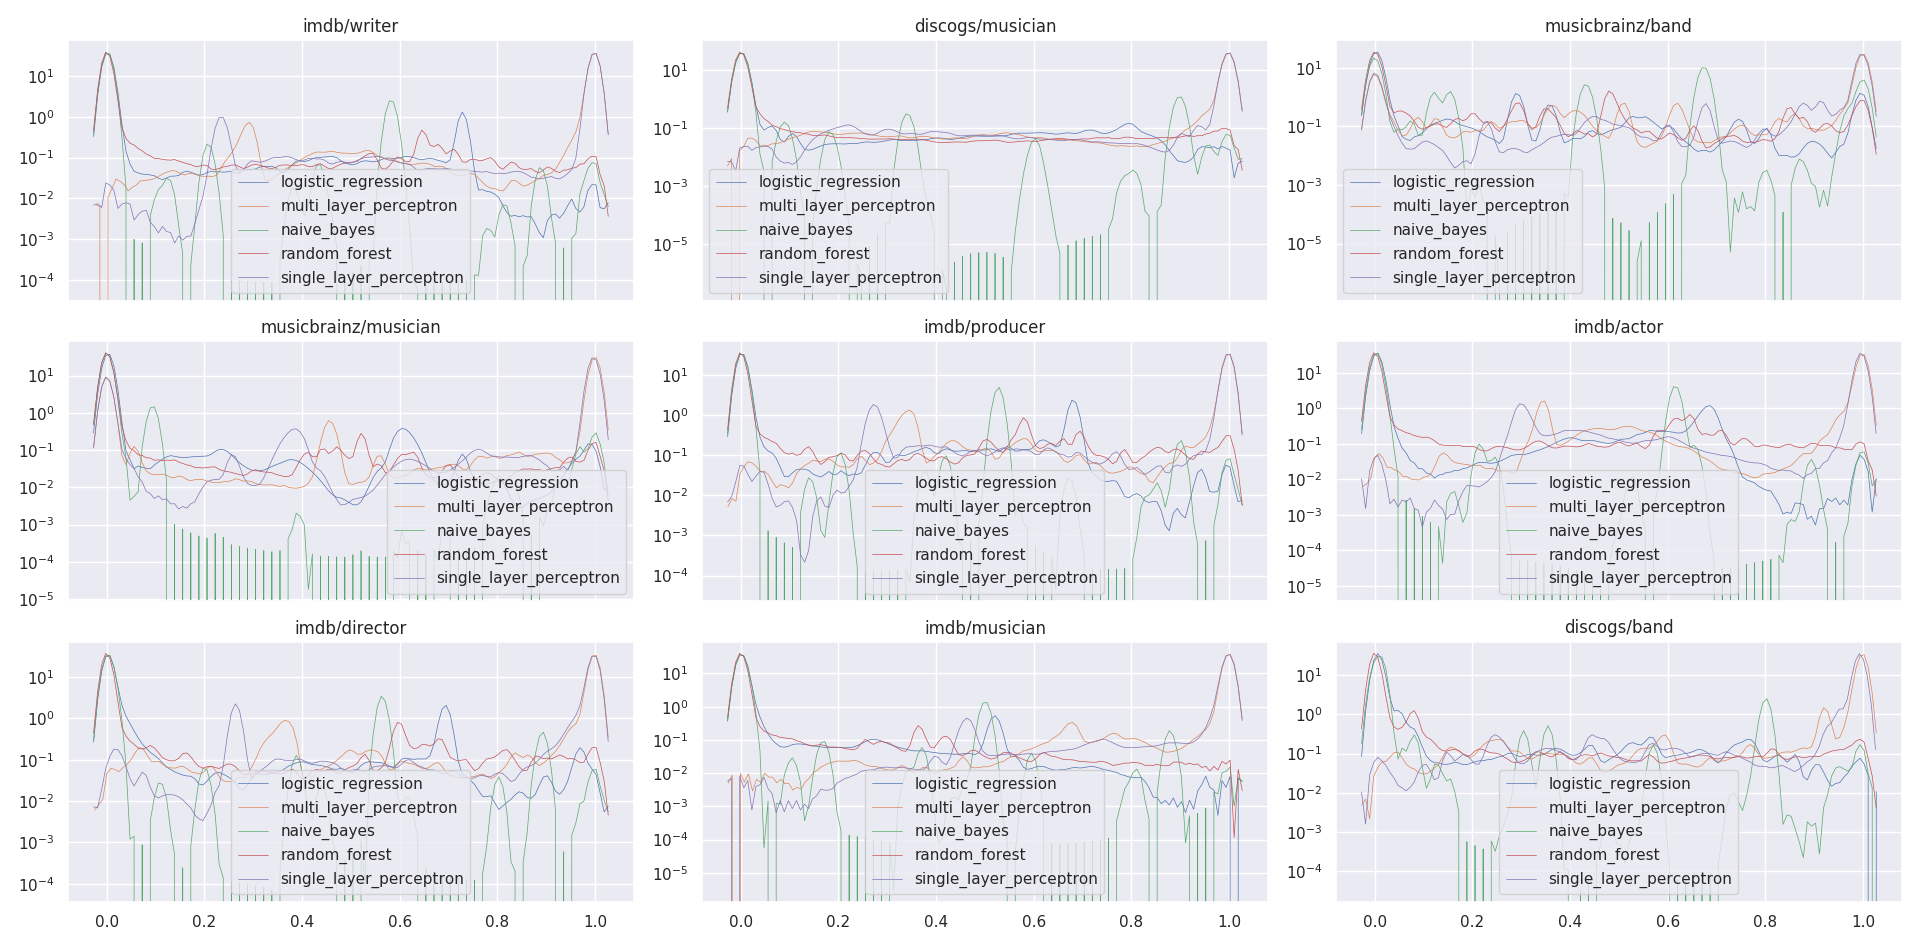
\includegraphics[width=\textwidth]{baseline_classification_continuous_classifiers_distplots} 
  \caption{Distribution of predictions for classifier whose output is in a binary space.}
  \label{fig:apx-baseline-classification-barplot}
\end{figure}

\begin{figure}[]
  \centering 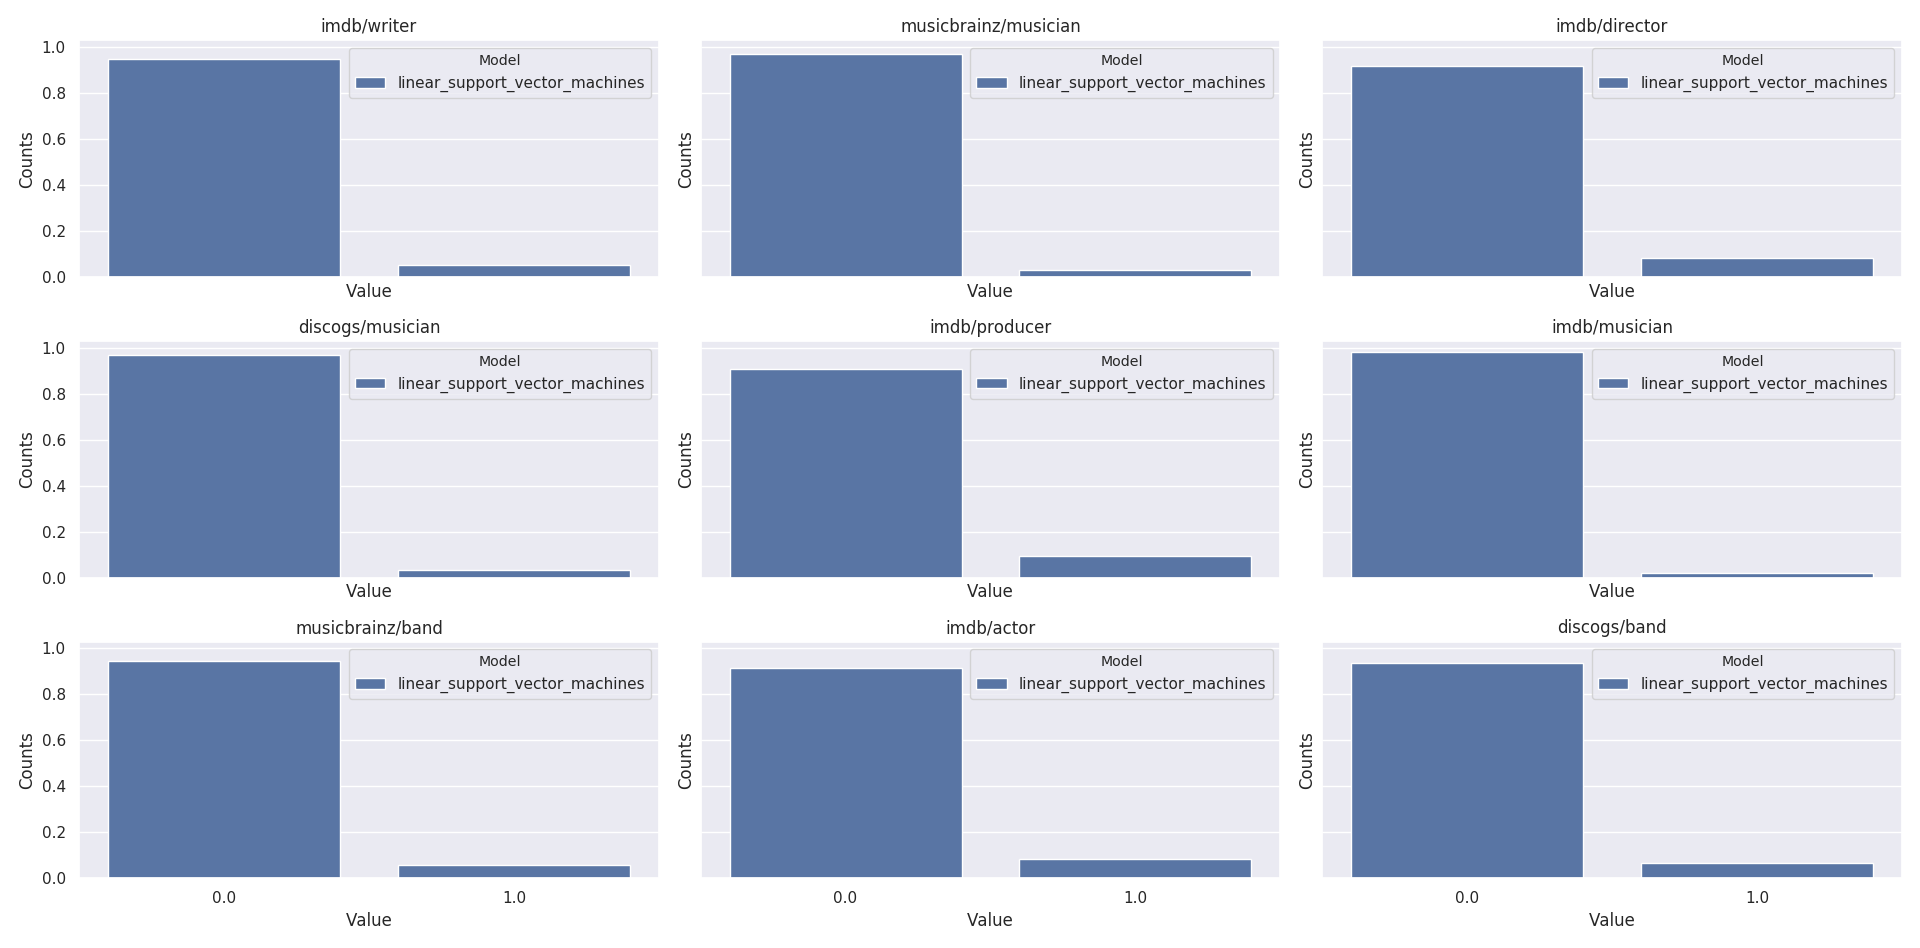
\includegraphics[width=\textwidth]{baseline_classification_binary_classifiers_barplot} 
  \caption{Distribution of predictions for classifier whose output is in a binary space.}
  \label{fig:apx-baseline-classification-barplot}
\end{figure}


\subsection{Ensembles classification results}
\label{sec:apx-ensembles-classification-results}


\begin{table}[H]
\centering
\begin{tabular}{|l|l|l|l|l|l|l|}
\hline
Model                    & Avg. Mean & Avg. STD & Avg. 25\% & Avg. 50\% & Avg. 75\% & Avg. Max \\ \hline
voting\_classifier\_soft & 0.057636     & 0.158270    & 0.003207     & 0.007516     & 0.021039     & 0.999121    \\
stacked\_classifier      & 0.056042     & 0.168406    & 0.009359     & 0.009674     & 0.011936     & 0.974617    \\
voting\_classifier\_hard & 0.054288     & 0.218717    & 0.000000     & 0.000000     & 0.000000     & 1.000000    \\
gated\_classifier        & 0.052910     & 0.167008    & 0.006857     & 0.007141     & 0.007596     & 0.989812    \\ \hline
\end{tabular}
\caption{}
\label{tab:apx-ensemble-classification-summary}
\end{table}

% consider name abbreviations!


\begin{longtable}{|l|l|l|l|l|l|l|l|l|l|l|}
\hline
Catalog     & Entity   & Model                    & Count  & Mean     & STD      & Min      & 25\%     & 50\%     & 75\%     & Max      \\ \hline
discogs     & musician & gc        & 515082 & 0.029858 & 0.134515 & 0.000000 & 0.005109 & 0.005152 & 0.005247 & 0.984798 \\
discogs     & band     & gc        & 92137  & 0.057388 & 0.179030 & 0.000000 & 0.009710 & 0.009955 & 0.010281 & 0.981458 \\
imdb        & actor    & gc        & 355515 & 0.065065 & 0.181855 & 0.005060 & 0.005130 & 0.005192 & 0.005239 & 0.987478 \\
imdb        & musician & gc        & 944196 & 0.017756 & 0.079748 & 0.004216 & 0.004266 & 0.004288 & 0.004328 & 0.988251 \\
imdb        & writer   & gc        & 68702  & 0.048981 & 0.170615 & 0.005432 & 0.005505 & 0.005550 & 0.005590 & 0.989302 \\
imdb        & producer & gc        & 9351   & 0.080576 & 0.213030 & 0.006867 & 0.007220 & 0.007352 & 0.007708 & 0.993112 \\
imdb        & director & gc        & 35094  & 0.066865 & 0.202458 & 0.005077 & 0.005161 & 0.005196 & 0.005438 & 0.983906 \\
musicbrainz & musician & gc        & 652175 & 0.027414 & 0.123071 & 0.000000 & 0.006402 & 0.006426 & 0.006457 & 1.000000 \\
musicbrainz & band     & gc        & 106026 & 0.082290 & 0.218746 & 0.000000 & 0.013210 & 0.015158 & 0.018073 & 1.000000 \\ \hline
discogs     & band     & sc      & 92137  & 0.054855 & 0.171827 & 0.000000 & 0.012356 & 0.012482 & 0.013273 & 0.959502 \\
discogs     & musician & sc      & 515082 & 0.023429 & 0.111203 & 0.000000 & 0.004903 & 0.004904 & 0.004925 & 0.956270 \\
imdb        & actor    & sc      & 355515 & 0.061541 & 0.175259 & 0.006668 & 0.006805 & 0.006814 & 0.007155 & 0.982776 \\
imdb        & producer & sc      & 9351   & 0.106723 & 0.253498 & 0.014097 & 0.014177 & 0.015255 & 0.018345 & 0.970012 \\
imdb        & musician & sc      & 944196 & 0.018207 & 0.082833 & 0.005190 & 0.005191 & 0.005253 & 0.005348 & 0.974544 \\
imdb        & director & sc      & 35094  & 0.061921 & 0.188322 & 0.005990 & 0.006000 & 0.006003 & 0.006119 & 0.956035 \\
imdb        & writer   & sc      & 68702  & 0.056798 & 0.194364 & 0.006776 & 0.006781 & 0.006801 & 0.007176 & 0.972416 \\
musicbrainz & musician & sc      & 652175 & 0.027208 & 0.115886 & 0.000000 & 0.009073 & 0.009075 & 0.009164 & 1.000000 \\
musicbrainz & band     & sc      & 106026 & 0.093695 & 0.222461 & 0.000000 & 0.018945 & 0.020480 & 0.035917 & 1.000000 \\ \hline
discogs     & band     & vh & 92137  & 0.057187 & 0.232200 & 0.000000 & 0.000000 & 0.000000 & 0.000000 & 1.000000 \\
discogs     & musician & vh & 515082 & 0.029859 & 0.170199 & 0.000000 & 0.000000 & 0.000000 & 0.000000 & 1.000000 \\
imdb        & musician & vh & 337111 & 0.017525 & 0.131219 & 0.000000 & 0.000000 & 0.000000 & 0.000000 & 1.000000 \\
imdb        & writer   & vh & 68702  & 0.048718 & 0.215279 & 0.000000 & 0.000000 & 0.000000 & 0.000000 & 1.000000 \\
imdb        & actor    & vh & 355515 & 0.083248 & 0.276257 & 0.000000 & 0.000000 & 0.000000 & 0.000000 & 1.000000 \\
imdb        & producer & vh & 9351   & 0.087156 & 0.282079 & 0.000000 & 0.000000 & 0.000000 & 0.000000 & 1.000000 \\
imdb        & director & vh & 35094  & 0.081125 & 0.273031 & 0.000000 & 0.000000 & 0.000000 & 0.000000 & 1.000000 \\
musicbrainz & band     & vh & 106026 & 0.061240 & 0.239771 & 0.000000 & 0.000000 & 0.000000 & 0.000000 & 1.000000 \\
musicbrainz & musician & vh & 652175 & 0.022537 & 0.148422 & 0.000000 & 0.000000 & 0.000000 & 0.000000 & 1.000000 \\ \hline
discogs     & band     & vs & 92137  & 0.063509 & 0.168745 & 0.000000 & 0.008184 & 0.012160 & 0.017549 & 0.999697 \\
discogs     & musician & vs & 515082 & 0.030028 & 0.133205 & 0.000000 & 0.001535 & 0.002331 & 0.004532 & 0.998474 \\
imdb        & musician & vs & 944196 & 0.021848 & 0.092686 & 0.000205 & 0.001234 & 0.001659 & 0.002589 & 0.999709 \\
imdb        & writer   & vs & 68702  & 0.043952 & 0.148484 & 0.000438 & 0.002171 & 0.002948 & 0.003702 & 0.999094 \\
imdb        & producer & vs & 9351   & 0.076109 & 0.182346 & 0.002841 & 0.006002 & 0.006845 & 0.009239 & 0.996601 \\
imdb        & actor    & vs & 355515 & 0.068285 & 0.185416 & 0.000203 & 0.002040 & 0.002958 & 0.004662 & 0.998976 \\
imdb        & director & vs & 35094  & 0.064267 & 0.185011 & 0.000541 & 0.002337 & 0.002876 & 0.007271 & 0.999539 \\
musicbrainz & band     & vs & 106026 & 0.126356 & 0.213054 & 0.000000 & 0.004267 & 0.034199 & 0.137530 & 1.000000 \\
musicbrainz & musician & vs & 652175 & 0.024370 & 0.115483 & 0.000000 & 0.001089 & 0.001672 & 0.002279 & 1.000000 \\ \hline
\end{longtable}

\begin{figure}[]
  \centering 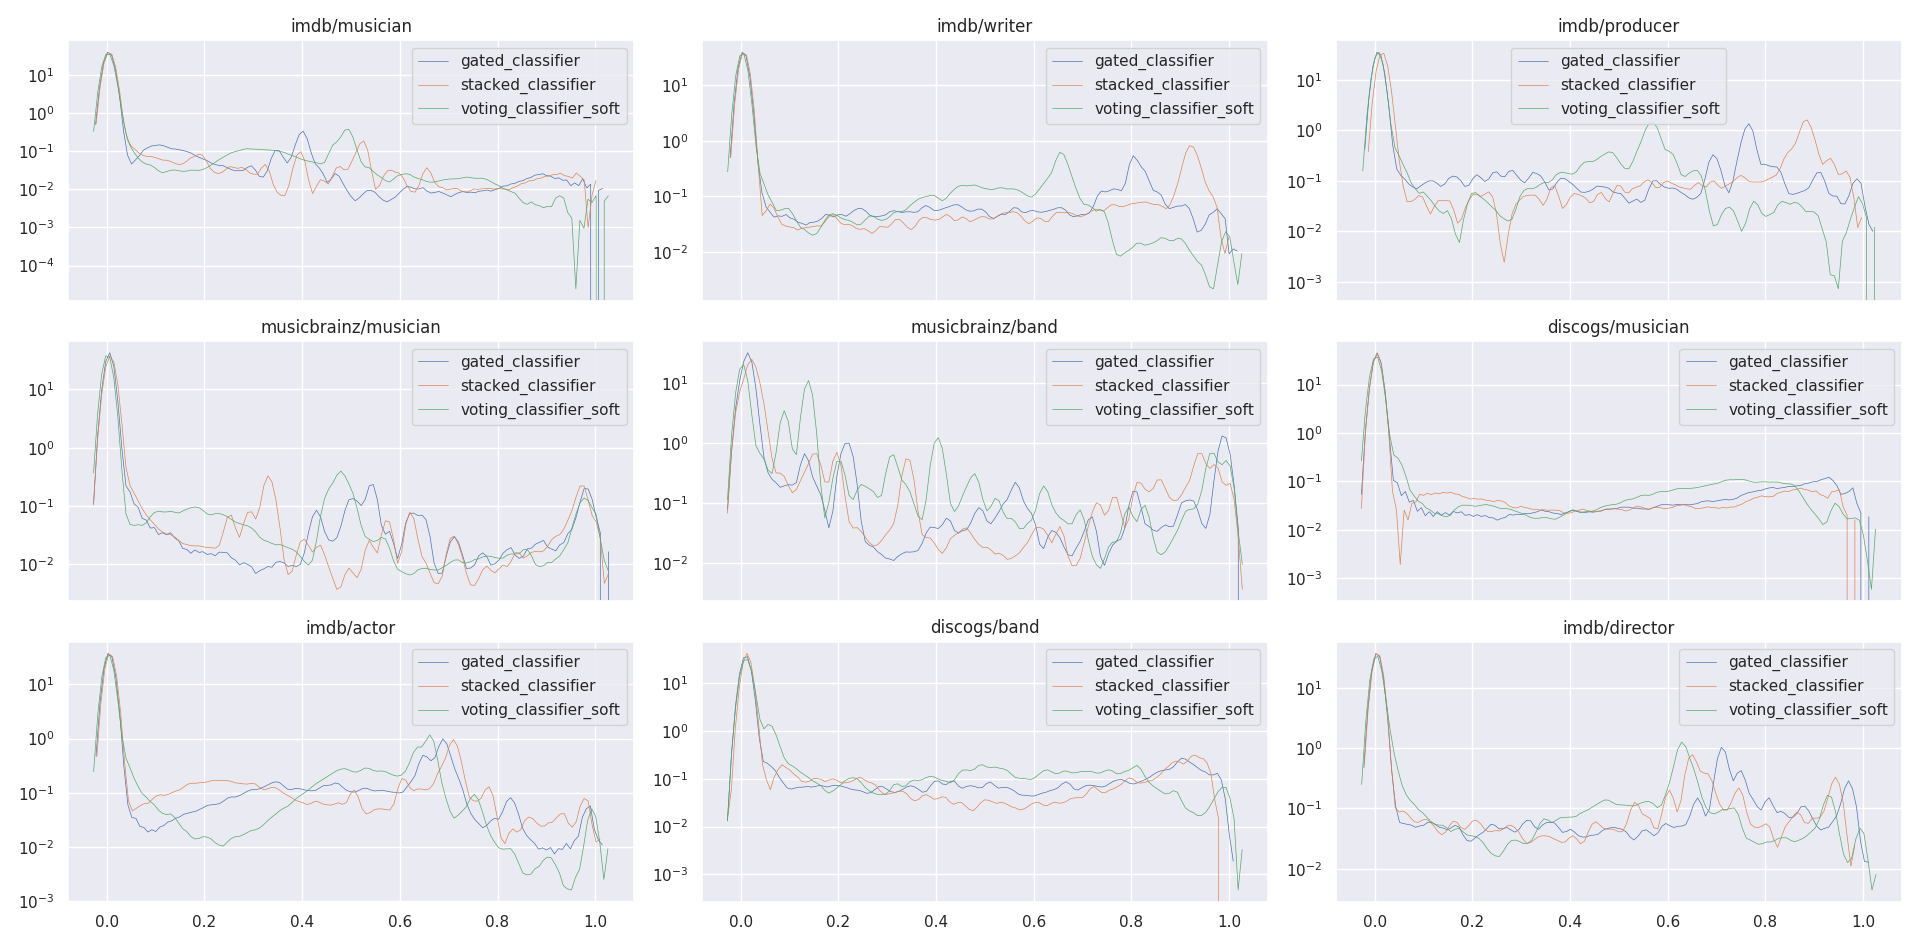
\includegraphics[width=\textwidth]{ensembles_classification_continuous_classifiers_distplots} 
  \caption{Distribution of predictions for classifiers whose output is in a continuous space.}
  \label{fig:apx-ensemble-classification-distplot}
\end{figure}

\begin{figure}[]
  \centering 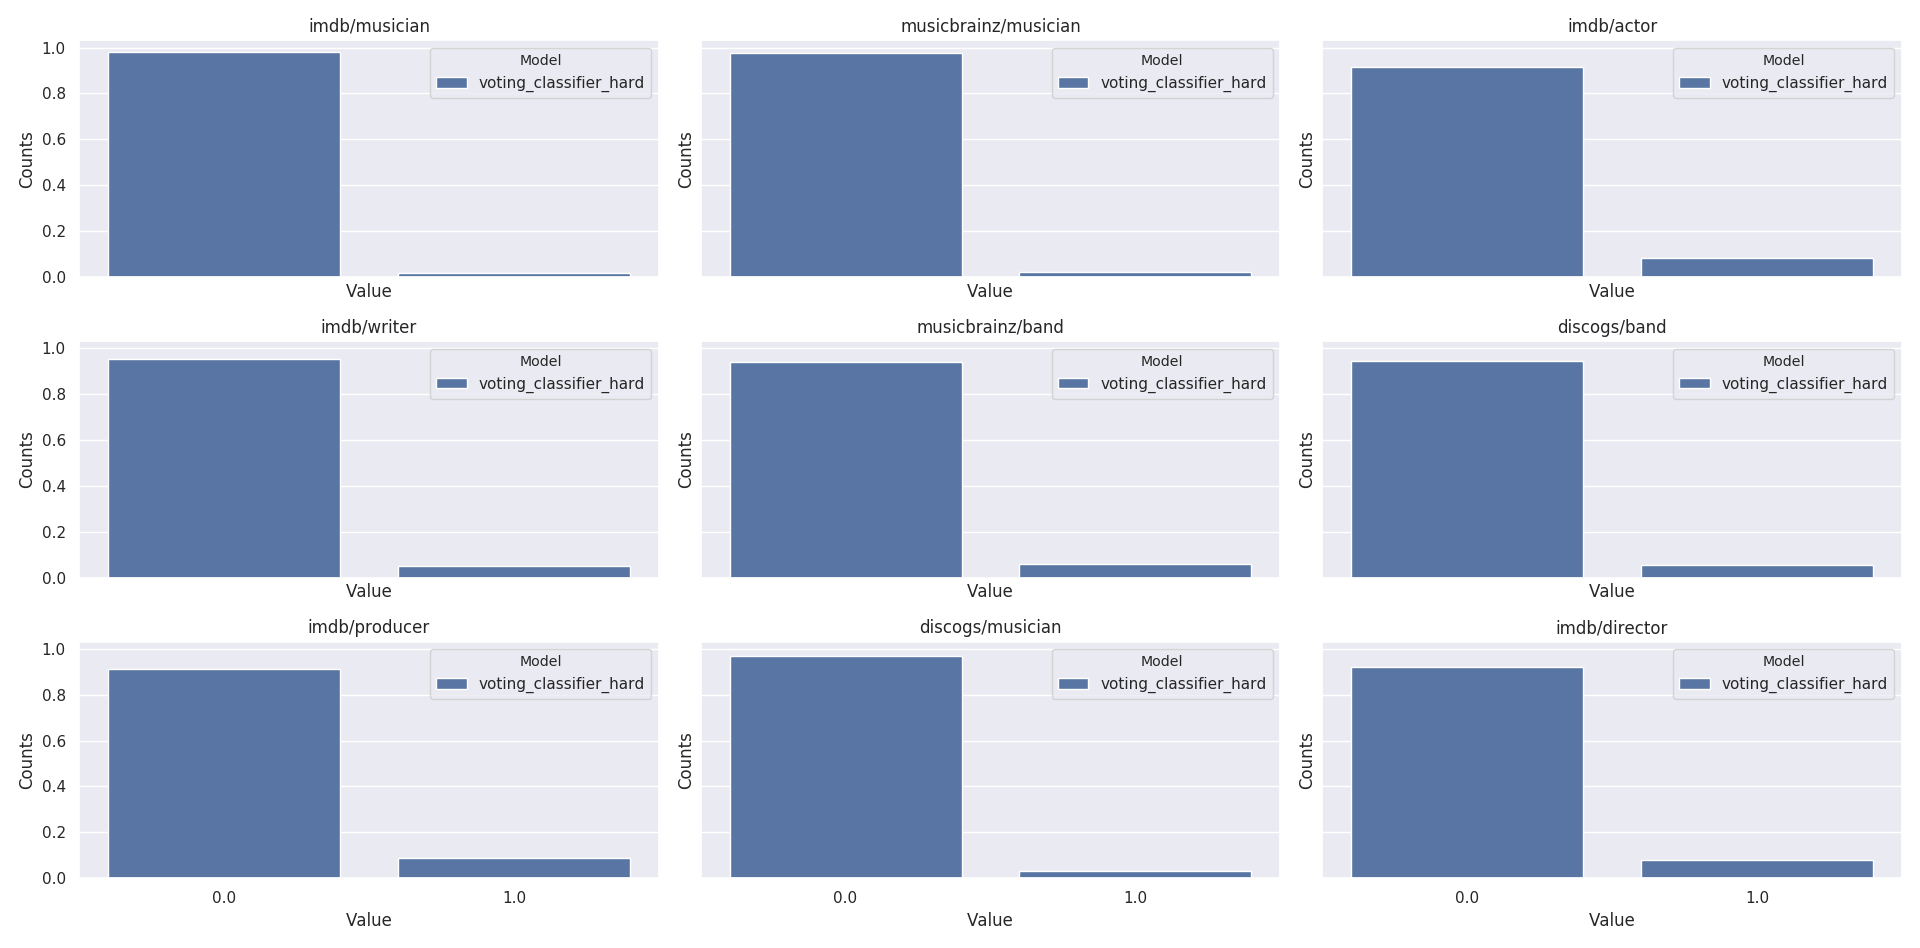
\includegraphics[width=\textwidth]{ensembles_classification_binary_classifiers_barplot} 
  \caption{Distribution of predictions for classifier whose output is in a binary space.}
  \label{fig:apx-ensemble-classification-barplot}
\end{figure}


\end{document}
